%% This is the ctufit-thesis example file. It is used to produce theses
%% for submission to Czech Technical University, Faculty of Information Technology.
%%
%% Get the newest version from
%% https://gitlab.fit.cvut.cz/theses-templates/FITthesis-LaTeX
%%
%%
%% Copyright 2021, Eliska Sestakova and Ondrej Guth
%%
%% This work may be distributed and/or modified under the
%% conditions of the LaTeX Project Public Licenese, either version 1.3
%% of this license or (at your option) any later version.
%% The latest version of this license is in
%%  https://www.latex-project.org/lppl.txt
%% and version 1.3 or later is part of all distributions of LaTeX
%% version 2005/12/01 or later.
%%
%% This work has the LPPL maintenance status `maintained'.
%%
%% The current maintainer of this work is Ondrej Guth.
%% Contact ondrej.guth@fit.cvut.cz for bug reports.
%% Alternatively, submit bug reports into the tracker at
%% https://gitlab.fit.cvut.cz/theses-templates/FITthesis-LaTeX/issues
%%
%%

%%%%%%%%%%%%%%%%%%%%%%%%%%%%%%%%%%%%%%%%%
% CLASS OPTIONS
% language: czech/english/slovak
% thesis type: bachelor/master/dissertation
%%%%%%%%%%%%%%%%%%%%%%%%%%%%%%%%%%%%%%%%%
\documentclass[czech,master,unicode,twoside]{ctufit-thesis}

% \geometry{textwidth=38em}
% \renewcommand{\baselinestretch}{1.15}
% \usepackage[letterspace=150]{microtype}

%%%%%%%%%%%%%%%%%%%%%%%%%%%%%%%%%%
% FILL IN THIS INFORMATION
%%%%%%%%%%%%%%%%%%%%%%%%%%%%%%%%%%
\ctufittitle{Platforma pro tvorbu interaktivních výukových materiálů} % replace with the title of your thesis
\ctufitauthorfull{Bc.\,Matěj Cajthaml} % replace with your full name (first name(s) and then family name(s) / surname(s)) including academic degrees
\ctufitauthorsurnames{Cajthaml} % replace with your surname(s) / family name(s)
\ctufitauthorgivennames{Matěj} % replace with your first name(s) / given name(s)
\ctufitsupervisor{Ing.\,Marek Suchánek, Ph.D. et Ph.D.} % replace with name of your supervisor/advisor (include academic degrees)
\ctufitdepartment{Katedra softwarového inženýrství} % replace with the department of your defence
\ctufitprogram{Informatika} % replace with your study program
\ctufitspecialisation{Webové inženýrství}
\ctufityear{2025} % replace with the year of your defence
\ctufitdeclarationplace{Praze} % replace with the place where you sign the declaration
\ctufitdeclarationdate{\today} % replace with the date of signature of the declaration
\ctufitabstractCZE{
Tato diplomová práce se věnuje analýze, návrhu a implementaci platformy pro tvorbu interaktivních studijních materiálů, jejímž cílem je zvýšit aktivní zapojení studentů do výuky. Klíčové části platformy jsou postaveny na architektuře Vue, NestJS a využívají WebSockets pro synchronizaci prezentací v~reálném čase. Podporuje skriptování pomocí komunitních rozšíření a umožňuje nejen tvorbu a prezentaci výukových materiálů, ale i~jejich sdílení, společnou editaci a sledování prezentací na zařízeních studentů. Součástí projektu je také prezentační web a technická dokumentace. Aplikace byla nasazena do produkčního prostředí a ověřena uživatelským testováním se studenty i~učiteli, doplněným o~automatizované testy.
}
\ctufitabstractENG{
This thesis focuses on the analysis, design and implementation of a platform for the creation of interactive learning materials aimed at increasing active student engagement in learning. The key parts of the platform are using Vue, NestJS and also WebSockets for real-time synchronization of presentations. It supports scripting with community extensions and allows not only creating and presenting learning materials, but also sharing, collaborative editing and viewing presentations on students' devices. The project also includes a presentation website and technical documentation. The application has been deployed in a production environment and validated by user testing with students and teachers, supplemented by automated tests.
}
\ctufitkeywordsCZE{materiály, prezentace, výuková platforma, interaktivita, zapojení studentů, webová aplikace, Vue, Nest, WebSockets}
\ctufitkeywordsENG{materials, presentation, learning platform, interactivity, student involvement, web application, Vue, Nest, WebSockets}
%%%%%%%%%%%%%%%%%%%%%%%%%%%%%%%%%%
% END FILL IN
%%%%%%%%%%%%%%%%%%%%%%%%%%%%%%%%%%

%%%%%%%%%%%%%%%%%%%%%%%%%%%%%%%%%%
% CUSTOMIZATION of this template
% Skip this part or alter it if you know what you are doing.
%%%%%%%%%%%%%%%%%%%%%%%%%%%%%%%%%%

\RequirePackage{iftex}[2020/03/06]
\iftutex % XeLaTeX and LuaLaTeX
    \RequirePackage{ellipsis}[2020/05/22] %ellipsis workaround for XeLaTeX
\else
    \errmessage{Only compilation with XeLaTeX or LuaLaTeX is allowed}
    \stop
\fi


% hyperlinks
% \hypersetup{
%     pdfpagelayout=TwoPageRight,
%     colorlinks=false,
%     allcolors=decoration,
%     pdfborder={0 0 0.1}
% }

% uncomment the following to hide all hyperlinks
\hypersetup{hidelinks}

% uncomment the following to change the colour of all hyperlinks to CTU blue
%\hypersetup{allbordercolors=decoration}

\RequirePackage{pdfpages}[2020/01/28]

\setcounter{secnumdepth}{4} % numbering sections; 4: subsubsection
\setcounter{tocdepth}{2}



%%%%%%%%%%%%%%%%%%%%%%%%%%%%%%%%%%
% CUSTOMIZATION of this template END
%%%%%%%%%%%%%%%%%%%%%%%%%%%%%%%%%%


%%%%%%%%%%%%%%%%%%%%%%
% DEMO CONTENTS SETTINGS
% You may choose to modify this part.
%%%%%%%%%%%%%%%%%%%%%%
% \usepackage{todonotes}
\usepackage{xevlna}
% \usepackage{lineno}
% \usepackage{parskip}
% \linenumbers

\usepackage{dirtree}
\usepackage{lipsum,tikz}
\usepackage{xurl}
\usepackage[style=iso-numeric]{biblatex}
\addbibresource{text/bib-database.bib}
\usepackage{listings} % typesetting of sources
\usepackage{minted} % typesetting of sources
\usepackage{longtable} % long talber
\usepackage{enumitem} % moving list
% \usepackage{tabularray}

\usepackage{amssymb}% http://ctan.org/pkg/amssymb
\usepackage{pifont}
\usepackage{graphicx}
 % \usepackage[table,xcdraw]{xcolor}

\usepackage{csquotes}
\usepackage{tablefootnote}
\newcommand{\cmark}{\ding{51}}
\newcommand{\xmark}{\ding{55}}

%theorems, definitions, etc. END
%%%%%%%%%%%%%%%%%%%%%%
% DEMO CONTENTS SETTINGS END
%%%%%%%%%%%%%%%%%%%%%%


\setlength{\headheight}{14.03358pt}
%\overfullrule=10pt

\begin{document} 
\frontmatter\frontmatterinit % do not remove these two commands
\thispagestyle{empty}\maketitle\thispagestyle{empty}\cleardoublepage % do not remove these four commands

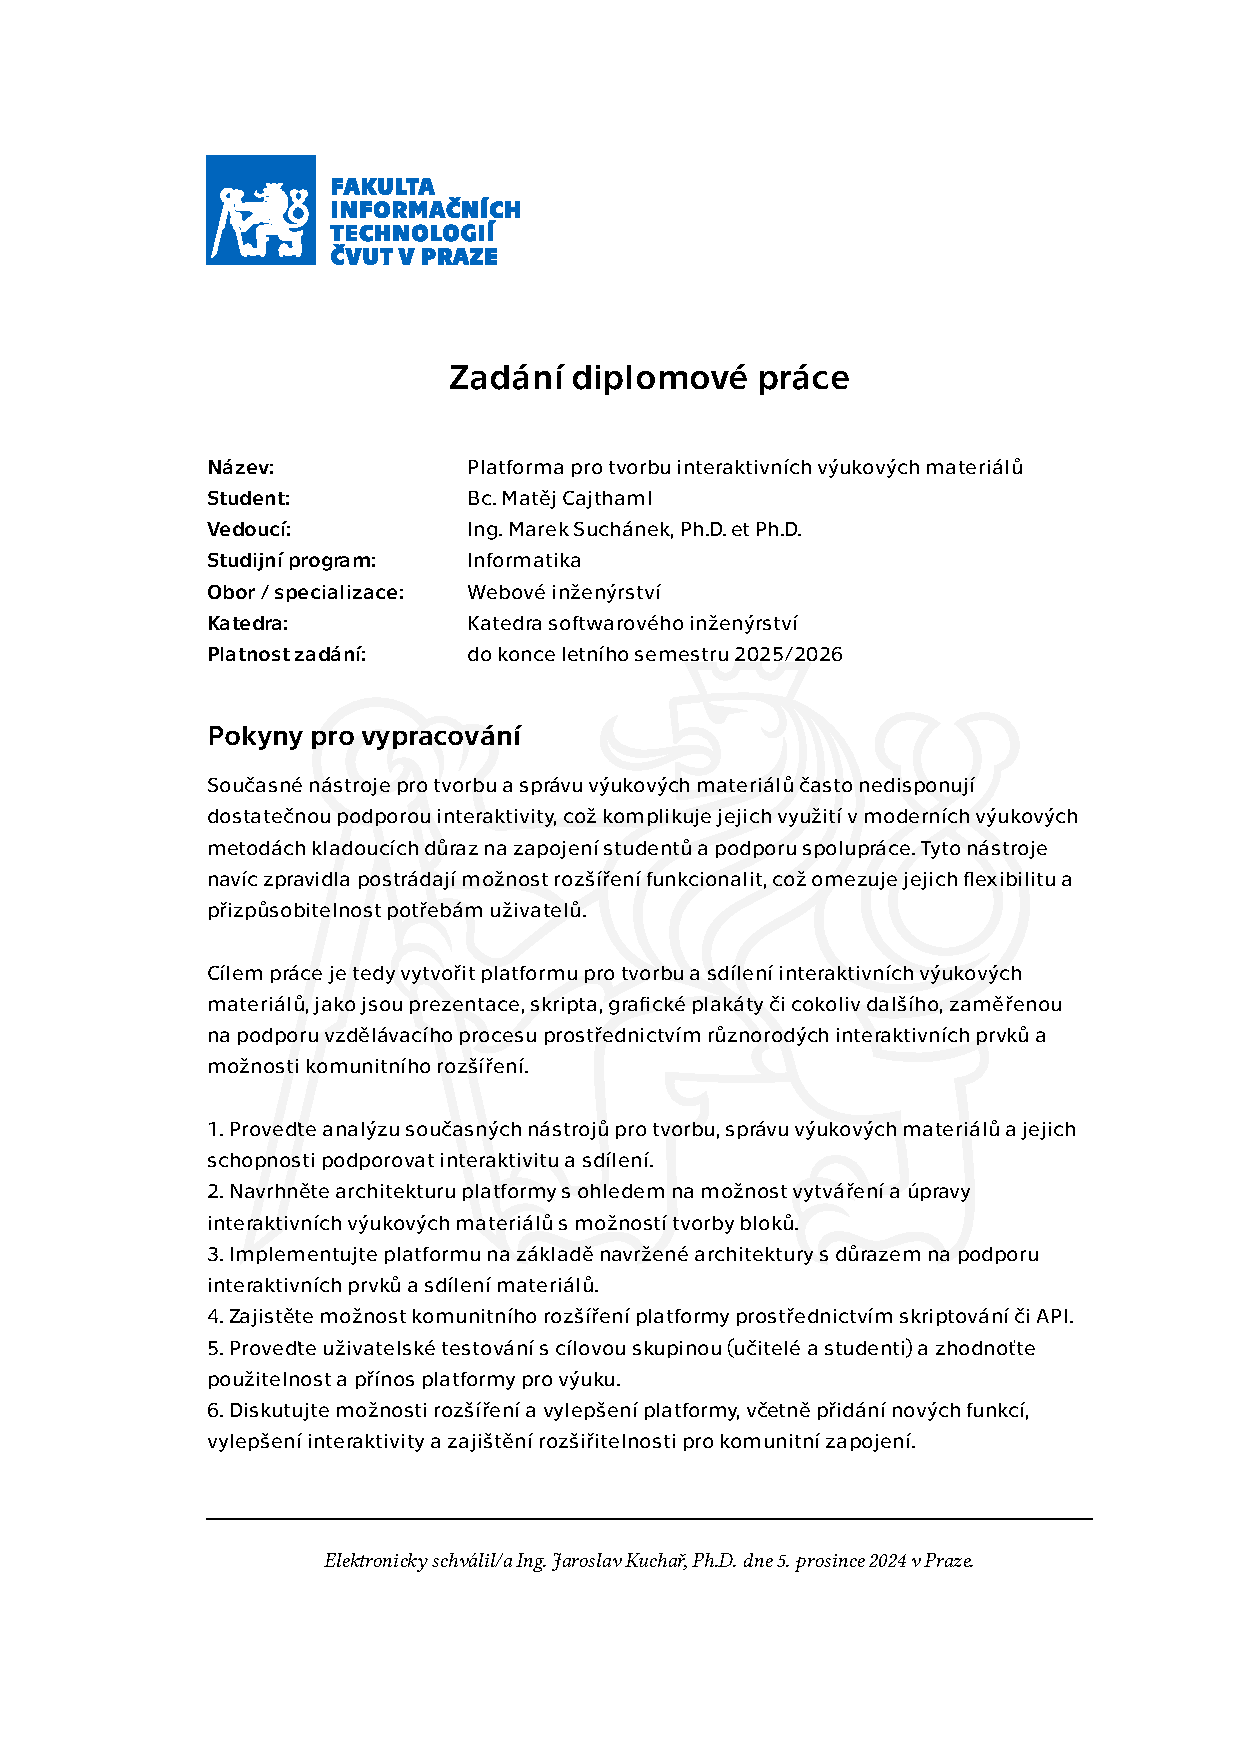
\includepdf[pages={1-}]{cajthmat-assignment.pdf} % replace this file with your thesis assignment generated from ProjectsFIT
% 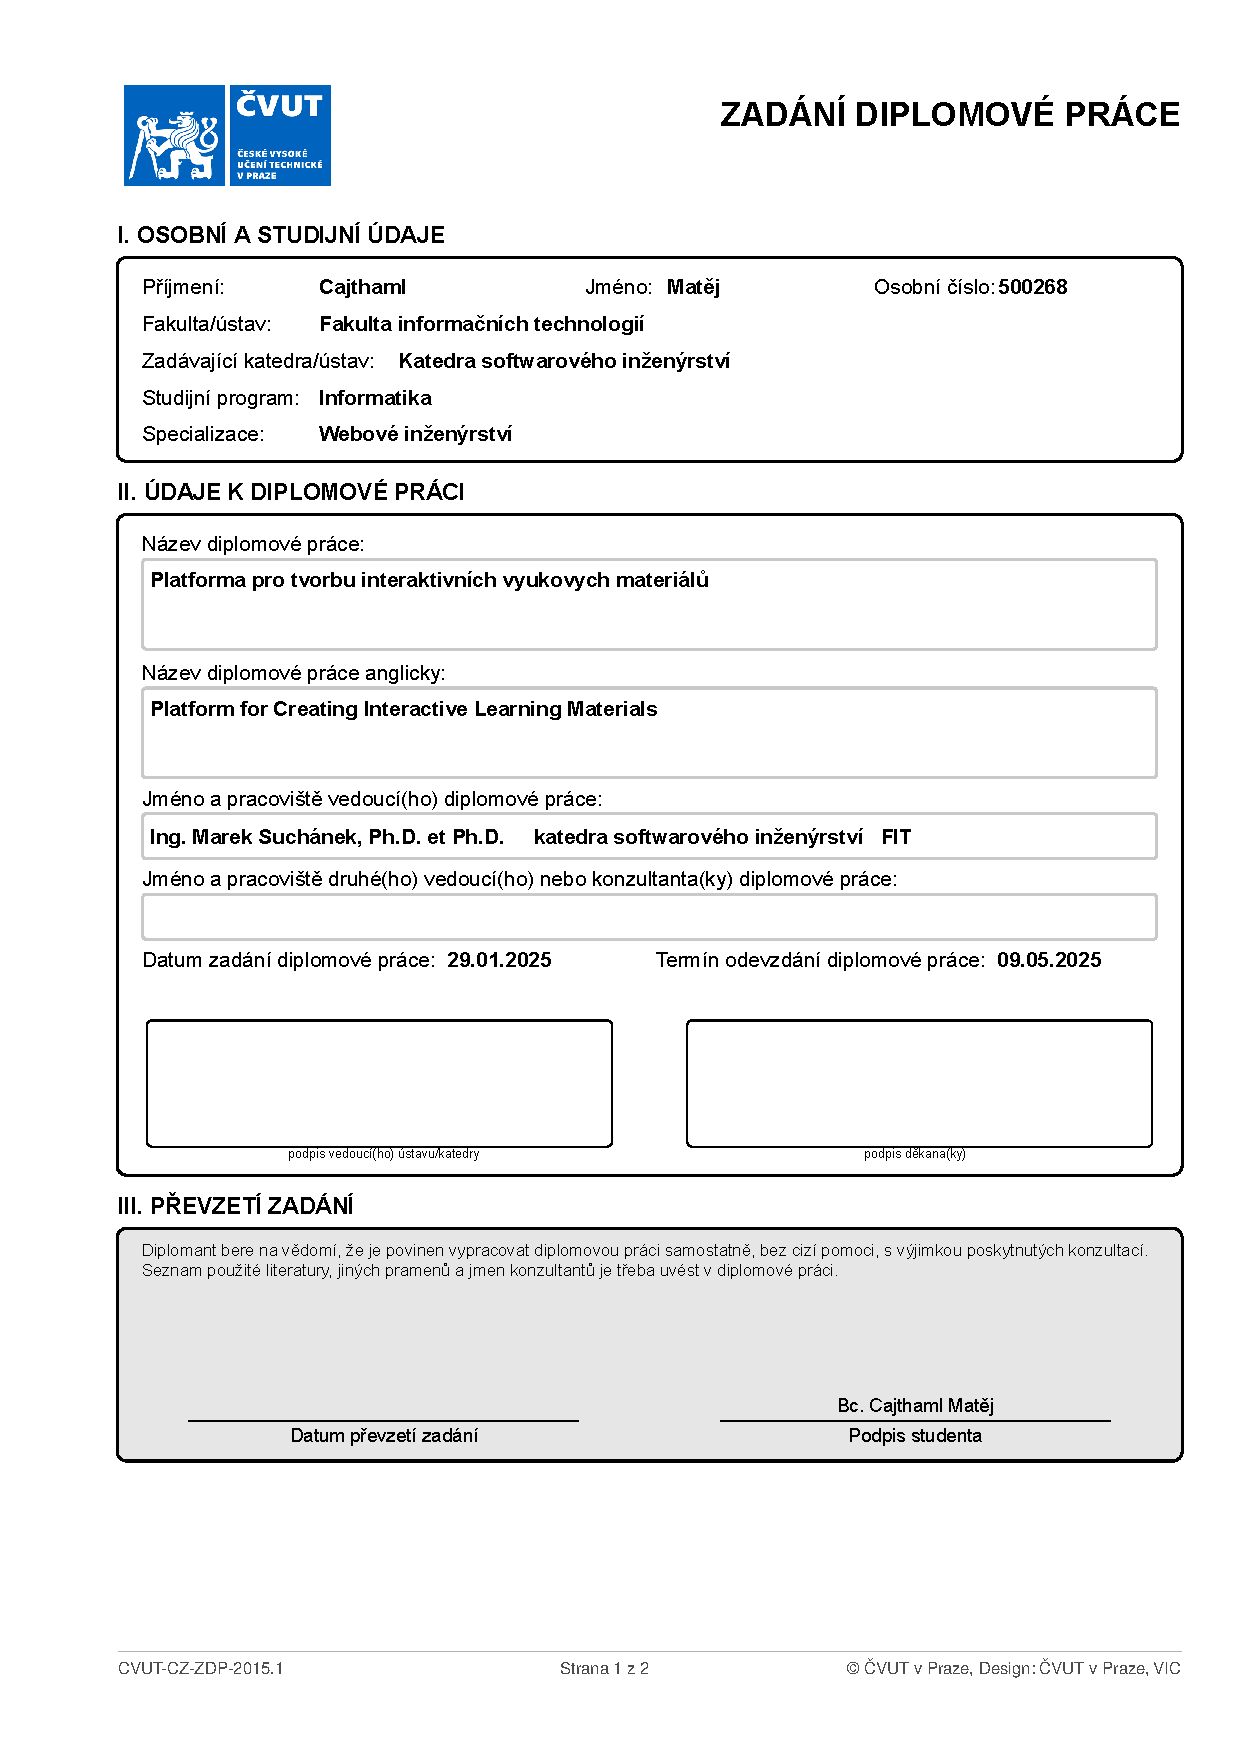
\includepdf[pages={1-}]{zadani.pdf} % replace this file with your thesis assignment generated from ProjectsFIT

\imprintpage % do not remove this command
\stopTOCentries

%%%%%%%%%%%%%%%%%%%
% ACKNOWLEDGMENT
% FILL IN / MODIFY
% This is a place to thank people for helping you. It is common to thank your supervisor.
%%%%%%%%%%%%%%%%%%%
\begin{acknowledgmentpage}
    Nejprve bych chtěl poděkovat vedoucímu mé diplomové práce, panu Ing.\,Marku Suchánkovi, Ph.D. et Ph.D., za možnost pracovat na využitelném projektu a také za všechny jeho cenné rady a konzultace, kterých se mi během psaní a realizace práce dostalo.

    \vspace{1em}
    
    Taktéž chci poděkovat všem svým přátelům a testerům, kteří mě v~práci podporovali, a práci mi průběžně kontrolovali. Zejména slečnám Kristýně Dřevikovské a Avě Špráchalů
    % a panu Denisovi Lengerovi 
    za jejich korekce a neustálou oporu. A také pánům
    Brodmanovi,
    Andrýskovi,
    Křemečkovi
    a
    Bruthansi 
    za pomoc během testování.

    \vspace{1em}

    Velké díky patří i~všem mým studentům, kteří mě zejména tento školní rok při práci podporovali, motivovali a vždy předávali cennou zpětnou vazbu. 
\end{acknowledgmentpage} 
%%%%%%%%%%%%%%%%%%%
% ACKNOWLEDGMENT END
%%%%%%%%%%%%%%%%%%%


%%%%%%%%%%%%%%%%%%%
% DECLARATION
% FILL IN / MODIFY
%%%%%%%%%%%%%%%%%%%
% INSTRUCTIONS
% ENG: choose one of approved texts of the declaration. DO NOT CREATE YOUR OWN. Find the approved texts at https://courses.fit.cvut.cz/SFE/download/index.html#_documents (document Declaration for FT in English)
% CZE/SLO: Vyberte jedno z~fakultou schvalenych prohlaseni. NEVKLADEJTE VLASTNI TEXT. Schvalena prohlaseni najdete zde: https://courses.fit.cvut.cz/SZZ/dokumenty/index.html#_dokumenty (prohlášení do ZP)
\begin{declarationpage}
Prohlašuji, že jsem předloženou práci vypracoval samostatně a že jsem uvedl veškeré
použité informační zdroje v~souladu s~Metodickým pokynem o~dodržování etických
principů při přípravě vysokoškolských závěrečných prací.
Beru na vědomí, že se na moji práci vztahují práva a povinnosti vyplývající ze zákona
č. 121/2000 Sb., autorského zákona, ve~znění pozdějších předpisů, zejména
skutečnost, že České vysoké učení technické v~Praze má právo na uzavření licenční
smlouvy o~užití této práce jako školního díla podle § 60 odst. 1 citovaného zákona.

\vspace{1em}

% Prohlašuji, že jsem v~průběhu příprav a psaní závěrečné práce použil nástroje umělé inteligence v~souladu s~Metodickým pokynem.
% Konkrétně šlo o~chytré doplňování kódu, úpravu a reformulaci textu. 
% Veškerý vygenerovaný obsah jsem samostatně ověřil a stvrzuji, že za jeho konečnou podobu a odbornou správnost plně zodpovídám.

Prohlašuji, že jsem v~průběhu příprav a psaní závěrečné práce použil nástroje umělé
inteligence. Vygenerovaný obsah jsem ověřil. 
Stvrzuji, že jsem si vědom, že za obsah závěrečné práce plně zodpovídám.
\end{declarationpage}
%%%%%%%%%%%%%%%%%%%
% DECLARATION END
%%%%%%%%%%%%%%%%%%%

\printabstractpage % do not remove this command

\tableofcontents % do not remove this command
%%%%%%%%%%%%%%%%%%%%%%
% list of other contents: figures, tables, code listings, algorithms, etc.
% add/remove commands accordingly
%%%%%%%%%%%%%%%%%%%%%%
\listoffigures % list of figures
\begingroup
\let\clearpage\relax
\listoftables % list of tables
\thectufitlistingscommand
\endgroup

%%%%%%%%%%%%%%%%%%%
% ABBREVIATIONS
% FILL IN / MODIFY
% OR REMOVE ENTIRELY
% List the abbreviations in lexicography order.
%%%%%%%%%%%%%%%%%%%
\chapter{\thectufitabbreviationlabel}
 
\begin{longtable}{rl}
% AJAX & Asynchronous JavaScript and XML\\
API & Application Programming Interface\\
CD & Content delivery\\
CI & Content integration\\
CORS & Cross-Origin Resource Sharing\\
CRUD & Create Read Update Delete\\
CSS & Cascading Style Sheets\\
% CSS3 & Cascading Style Sheets verze 3\\
% CSV & Comma separated values\\
% ČVUT & České vysoké učení technické\\
DI & Dependency Injection\\
DOM & Document Object Model\\
DTO & Data Transfer Object\\
E2E & End-to-end\\
% FIT & Fakulta informačních technologií\\
% GUI & Graphical User Interface\\
HTML & HyperText Markup Language\\
% HTML5 & HyperText Markup Language verze 5\\
HTTP & Hypertext Transfer Protocol\\
HTTPS & Hypertext Transfer Protocol Secure\\
% IS & Informační systém\\
IDE & Integrated Development Environment\\
JS & JavaScript\\
JSON & JavaScript Object Notation\\
% JSX & JavaScript Syntax Extension\\
JWT & JSON Web Token\\
% Less & Leaner Style Sheets\\
MS & Microsoft\\
% NoSQL & Not only SQL\\
% npm & Node Package Manager\\
ODM & Object Document Mapping\\
ORM & Object Relation Mapping\\
PDF & Portable Document Format\\
SQL & Structured Query Language\\
% REST & Representational State Transfer\\
Sass & Syntactically awesome style sheets\\
% SEO & Search Engine Optimalization\\
SOAP & Simple Object Access Protocol\\
SPA & Single Page Application\\
SVG & Scalable Vector Graphics\\
SŘBD & Systém řízení báze dat\\
SSPŠ & Smíchovská střední průmyslová škola a gymnázia\\
% SSR & Server-side rendering\\
% ŠIS & Školní informační systém\\
TS & TypeScript\\
UI & User Interface\\
UX & User Experience\\
% URI & Uinform Resource Identificator\\
URL & Uniform Resource Locator\\
% WWW & World Wide Web\\
% WYSIWYG & What you see is what you get\\
% WYSIWYM & What you see is what you mean\\
% W3C & World Wide Web Consortium\\
WS & Web sockets\\
XML & Extensible Markup Language\\
XSS & Cross-site scripting
\end{longtable}
%%%%%%%%%%%%%%%%%%%
% ABBREVIATIONS END
%%%%%%%%%%%%%%%%%%%

\resumeTOCentries
\mainmatter\mainmatterinit % do not remove these two commands
%%%%%%%%%%%%%%%%%%%
% THE THESIS
% MODIFY ANYTHING BELOW THIS LINE
%%%%%%%%%%%%%%%%%%%
\chapter*{Úvod}\addcontentsline{toc}{chapter}{Úvod}\markboth{Úvod}{Úvod}
%---------------------------------------------------------------
\setcounter{page}{1}

% Jednou z nejdůležitějších výzev moderního vzdělávání je tvorba efektivních a atraktivních vzdělávacích materiálů.
% Jako pedagog na střední škole si denně uvědomuji, jak náročné je nejen vytvářet, ale i udržovat materiály, které skutečně podporují vzdělávací proces.
% V dnešní době, kdy jsou tradiční formáty, jako například pasivní čtení prezentací, vnímány jako neefektivní a klasická skripta často studenty nezaujmou, je stále naléhavější potřeba využívat moderní a interaktivní přístupy, které dokážou lépe zapojit studenty.

% Současné nástroje pro tvorbu a správu výukových materiálů často postrádají dostatečnou podporu interaktivity a flexibility, což značně omezuje jejich využitelnost v moderních vyučovacích metodách.
% Tyto nedostatky přinášejí výzvy nejen vyučujícím, ale i samotným studentům, kteří potřebují materiály, jež odpovídají dynamice současných vzdělávacích procesů ale i jejich potřebám.
% Navíc možnosti rozšíření stávajících nástrojů bývají omezené, což komplikuje jejich přizpůsobení specifickým potřebám pedagogů.

% Cílem této práce je vytvořit inovativní platformu pro tvorbu a sdílení interaktivních vzdělávacích materiálů, která se zaměří na zlepšení vzdělávacího procesu prostřednictvím různorodých interaktivních prvků.
% Tato platforma by měla poskytovat podporu pro širokou škálu materiálů, od prezentací přes skripta až po vizuální plakáty, a umožnit jejich snadnou úpravu a sdílení.
% Součástí návrhu bude také systém komunitní rozšiřitelnosti, který podpoří dlouhodobý rozvoj platformy.

% Vývoj této platformy vychází z mé vlastní zkušenosti pedagoga, který na denní bázi pracuje se studenty a snaží se jim předávat znalosti co nejefektivněji. 
% Mnoho existujících nástrojů není schopno plně pokrýt potřeby moderní výuky a já i moji studenti často vnímáme jejich limity.
% S tvorbou platforem pro podporu výuky mám zkušenosti z dřívějších projektů, zejména z mé bakalářské práce~\cite{cajthaml_bp}, která implementovala studijní portál pro sdílení hodnocení, materiálů, poskytování služeb a například motivační prvky.
% Vytvoření platformy, která by zjednodušila proces tvorby materiálů a zároveň zvýšila jejich atraktivitu, představuje příležitost nejen pro mou práci a školu, ale i pro širokou pedagogickou komunitu.

% Magisterská práce bude zahrnovat analýzu existujících nástrojů, návrh architektury platformy a její implementaci s důrazem na interaktivitu a uživatelskou přívětivost.
% Výsledná platforma bude testována s cílovými skupinami, tedy učiteli a studenty, aby byla zajištěna její praktičnost a přínosnost.
% V neposlední řadě bude diskutována i budoucí rozšiřitelnost a možnosti zapojení širší pedagogické komunity.

% Tímto způsobem se snažím přispět ke zkvalitnění vzdělávacího procesu a podpořit efektivní využívání moderních technologií ve vzdělávání, čímž bych chtěl usnadnit práci nejen sobě, ale i dalším pedagogům, kteří čelí podobným výzvám.
% % \chapter*{Cíle}\addcontentsline{toc}{chapter}{Cíle}\markboth{Cíle}{Cíle}

% Cíle
\chapter{Analýza}\label{text:analyza}

\begin{chapterabstract}
Tato kapitola analyzuje nástroje a frameworky pro tvorbu a správu výukových materiálů, včetně jejich předností, nedostatků a podpory interaktivity. 
Zaměřuje se na tradiční i moderní nástroje a otázky vykreslování obsahu, komunitního rozšíření a bezpečnosti. 
V závěru jsou definovány klíčové požadavky na uživatele aplikace a funkčnosti, které je třeba řešit při návrhu platformy.
\end{chapterabstract}


\section{Správa a tvorba materiálů pro výuku}

Do vzdělávacího procesu mimo klasické metody patří tvorba a distribuce výukových materiálů.
Mezi výukové materiály lze zahrnout například prezentace, skripta, plakáty, interaktivní hry, doplňovačky, testy, simulační modely nebo audiovizuální obsah.
V posledních letech, díky rozvoji digitálních technologií, je stále důležitější sdílet materiály online, aby studenti mohli pracovat samostatně nebo v týmech a měli k materiálům přístup kdykoliv.

Online sdílení materiálů umožňuje rychlou aktualizaci obsahu, což je zvlášť důležité v případech, kdy se výukový obsah mění nebo vyvíjí v reakci na aktuální potřeby studentů nebo průběh výuky.
Navíc umožňuje učitelům flexibilně přizpůsobovat obsah individuálním potřebám jednotlivých studentů nebo skupin.
Studenti se poté cítí, že mohou studovat či si připomenout látku kdekoliv.

Dalším přínosem je možnost zpětné vazby v reálném čase, kdy studenti mohou přímo komentovat, odpovídat a reagovat na obsah materiálu.

Mezi platformy vhodné pro distribuci~\cite{msmt_aplikace} výukových materiálů patří například Microsoft Teams, Bakaláři, Google Disk a Google Classroom, Škola Online nebo další obdobné služby.
Tyto platformy často umožňují integraci s jinými nástroji, jako jsou kalendáře, nástroje pro komunikaci nebo aplikace na zadávání úkolů, což zjednodušuje organizaci výukového procesu.

Každá z těchto platforem má své specifické funkce -- například Microsoft Teams podporuje synchronní i asynchronní komunikaci mezi učiteli a studenty~\cite{teams}, zatímco Google Disk poskytuje možnost snadného sdílení a spolupráce na dokumentech v reálném čase.
V některých případech však tyto nástroje mohou být omezené, například z hlediska podpory různorodých formátů materiálů nebo absence pokročilých funkcí pro práci s interaktivními prvky.

I když se tato práce primárně nezabývá distribucí materiálů, je nezbytné, aby navrhovaná aplikace umožňovala sdílení obsahu pomocí odkazů.
Potom aplikace může sloužit jako další místo, na které budou z jiných aplikací učitelé ukazovat.

Nástroje pro tvorbu výukových materiálů zahrnují Google Slides, PowerPoint, Microsoft Word, \LaTeX, Canva a mnoho dalších, což podrobněji rozebírám v následujících kapitolách.
Učitelé často využívají širokou škálu nástrojů, protože žádný z existujících nástrojů není zcela dokonalý a není jednoduché vytvořit univerzální řešení.
Problém bývá, že různé typy materiálů jsou ve spoustě různých formátů, kde některé nepodporují interaktivní vzdělávání.
To způsobuje nejen značnou míru zmatení u studentů, ale i ztěžuje práci učitelům s různými platformami.

\subsection{Vlastní zkušenosti}

Žádná z klasických platforem na sdílení výukových materiálů a hodnocení mi plně nevyhovovala~\cite{cajthaml_bp}, což mě vedlo k tomu, abych si v rámci své bakalářské práce vytvořil vlastní portál.
Tento portál umožňuje nejen sdílení materiálů, ale také zajišťuje automatickou interaktivitu, například tím, že si studenti mohou během hodiny zapisovat poznámky přímo do systému k danému materiálu.
Taktéž poskytuje mnoho dalších věcí, jako flexibilní hodnocení či motivační a gamifikační prvky.

V minulosti jsem používal v podstatě všechny nástroje zmíněné dříve i později, ať už pro tvorbu materiálů, jejich sdílení nebo interaktivní výuku.

Pro prezentace nyní často využívám RevealJS, který však má jistá omezení, jak podrobněji rozebírám v kapitole~\ref{text:revealjs}.
Skripta vytvářím buď přímo ve svém systému, nebo za pomoci \LaTeX, a pro tvorbu herních a interaktivních aktivit používám nástroje jako Blooket, JeopardyLabs a mnoho dalších služeb.

Rozdělení různých typů materiálů do více platforem mi však nevyhovuje, protože jejich správa je zbytečně složitá a časově náročná.
Právě tato zkušenost vedla k záměru této diplomové práce, jejímž cílem je vytvořit jednotnou platformu, která spojí různé typy materiálů a umožní jejich snadné rozšíření a úpravy.
To by mi (a doufám i dalším učitelům) pomohlo tvořit kvalitní, ale i interaktivní a hezké materiály pro různé účely.
Podobné názory mají i moje kolegyně a kolegové na Smíchovské průmyslové škole a gymnáziu, kde je cílem školy vytvořit co nejvíce individuální vzdělávání pro každého studenta.

Ze zpětných vazeb studentů, které pravidelně sbírám na konci pololetí a školního roku, často zaznívá, že interaktivita materiálů je nedostatečná a že jejich používání je kvůli tomu složité a neintuitivní.
Tato zpětná vazba dále zdůrazňuje potřebu vytvořit systém, který by byl přehledný, interaktivní a přizpůsobitelný jak pro učitele, tak pro studenty.

% \subsection{Dotazník}

% Prozatím si nejsem jistý, zda je to dobrý nápad.\todo{Provést?}

\section{Aplikace na tvorbu prezentací}\label{text:analyza/prezentace}

Nejpřirozenějším základem pro výuku je prezentace, která podporuje a vizualizuje myšlenky učitele před skupinou studentů.
Správně strukturovaná prezentace poskytuje kostru výkladu, umožňuje přehledné předání látky a pomáhá udržet pozornost publika.
Na trhu existuje celá řada nástrojů určených pro tvorbu prezentací, lišících se funkcionalitou, mírou interaktivity, možnostmi spolupráce a také obtížností při vytváření obsahu.
Následující podkapitoly popisují vybrané zástupce, kteří jsou pro mou budoucí práci relevantní.

\subsection{PowerPoint}

PowerPoint, součást balíku Microsoft Office, je dlouhodobě vnímán jako standard~\cite{pp_usage} v oblasti tvorby prezentací.
Mnoho uživatelů jej zná díky intuitivnímu rozhraní a širokému spektru funkcí~\cite{pp_usage}.
Hlavní výhody PowerPointu spočívají v jeho univerzálnosti, snadné obsluze a perfektní provázanosti s dalšími nástroji Microsoft Office, jako jsou Word či Excel~\cite{pp_excel, pp_word}.
Nabízí také velkou knihovnu šablon, grafů, přechodových efektů a základní možnosti vkládání multimédií.

Nevýhodou může být omezená kreativita u některých uživatelů vyplývající z lineárního uspořádání snímků a složitého nebo omezeného používání interaktivních prvků. 
Častým problémem je i kompatibilita mezi staršími a novějšími verzemi formátů.
Přestože PowerPoint existuje i ve webové verzi umožňující spolupráci v reálném čase, tato online varianta je funkcemi oproti desktopové verzi značně omezena~\cite{pp_platforms}.
Další nevýhodou je cena –- přístup k plné verzi aplikace je placený, a to často brzdí její širší využití zejména ve školách s omezenými rozpočty.

\subsection{Google Slides}\label{text:google_slides}

Google Slides je bezplatný webový nástroj pro tvorbu prezentací od společnosti Google. 
Hlavní přednosti spočívají v možnostech snadné spolupráce více uživatelů v reálném čase~\cite{slides}, neboť dokument lze sdílet a společně editovat odkudkoli.
Integrace s ostatními službami Google (Disk, Dokumenty, Tabulky) umožňuje jednoduchý import a export různých typů souborů a díky tomu se výrazně usnadňuje týmová práce a přístup ke společným materiálům. 
Podobně jsou implementovány integrace s komunitními rozšířeními ze služeb Google.
Ve výchozím stavu je služba zdarma, avšak pokročilé funkce a správa dat jsou často vázány na účet v rámci Google Workspace~\cite{slides}, který mohou organizace platit v rámci firemního nebo institucionálního předplatného. 

Výhodou je automatické ukládání na cloud, takže není nutné se obávat ztráty dat~\cite{slides}, a navíc je vše dostupné na více zařízeních, což usnadňuje vzdálený přístup k prezentacím. 
Na druhou stranu je nezbytné mít stabilní připojení k internetu a být obezřetný vůči ukládání citlivých údajů do cloudu, protože Google Slides shromažďuje metadata o aktivitě uživatelů (například informace o tom, kdo a kdy dokument editoval)~\cite{google_terms}, což může s ohledem na soukromí a bezpečnost některým institucím či uživatelům vadit. 
Dále je možné, že prezentace vytvořené v Google Slides nebudou stoprocentně kompatibilní s PowerPointem a jinými nástroji zejména ve své interaktivitě a pluginy, což může způsobit problémy při přenosu mezi různými platformami. 
Nevýhodou jsou také omezenější pokročilé funkce, animace či grafické úpravy oproti PowerPointu nebo jiným specializovaným nástrojům. 

Google Slides nicméně celkově nabízí snadno použitelný a přístupný nástroj pro spolupráci a rychlou tvorbu prezentací, který uživatelům postačí pro většinu běžných scénářů, obzvláště tam, kde je důraz na flexibilitu, týmovou práci a okamžitý vzdálený přístup k materiálům.


\subsection{RevealJS}\label{text:revealjs}

RevealJS je knihovna a framework, která dovoluje tvořit prezentace pomocí zdrojového kódu v \texttt{HTML}. 
Výsledné prezentace jsou k dispozici jako webová stránka~\cite{revealjs}, ve které se vykreslují jednotlivé snímky, mezi kterými lze plynule procházet. 
Velkou výhodou RevealJS je široká komunita, řada open-source pluginů a neomezené možnosti integrace multimediálního obsahu, od videí přes animace až po spustitelný kód. 
Nevýhodou může být různé zpracování, dokumentace a nastavení pluginů, které nemusí být vždy vzájemně kompatibilní, nutnost znalostí webových technologií a absence \texttt{WYSIWYG} editoru. 

Vytvořené prezentace je často nutné hostovat na cloudu, zejména pokud používají pluginy vyžadující serverové prostředí.
Společnost, která vytvořila RevealJS, taktéž vytvořila službu Slides.com~\cite{revealjs, slidescom}, umožňující tvořit prezentace pomocí editoru s frameworkem RevealJS, s prémiovými pluginy a automatickým cloudovým uložením, avšak tento nástroj je kódově uzavřený a placený. 

Osobně jsem RevealJS knihovnu již řadu let používal pro tvorbu prezentací pro své studenty, kteří ocenili možnost vytvářet v prezentaci interaktivní prvky, jako je například kódový blok s okamžitým zobrazením výsledku. 
Na obrázku \ref{fig:analyza:revealjs-ukazka} je vidět příklad takové prezentace, kde je vlevo kód a vpravo výsledek zobrazený v prohlížeči, což podporuje lepší pochopení učiva a aktivní zapojení studentů. 

Zajímavou funkcí jsou i tzv. vertikální snímky, které umožňují nelineární strukturování prezentace, kdy se lze pohybovat nejen horizontálně, ale i vertikálně v rámci logických celků prezentace.
Celkově si uživatelé chválí i možnost modularity těchto snímků a že je velmi jednoduché spojovat jednotlivé atomické skupiny do větších celků.


\begin{figure}[h!]
    \centering
    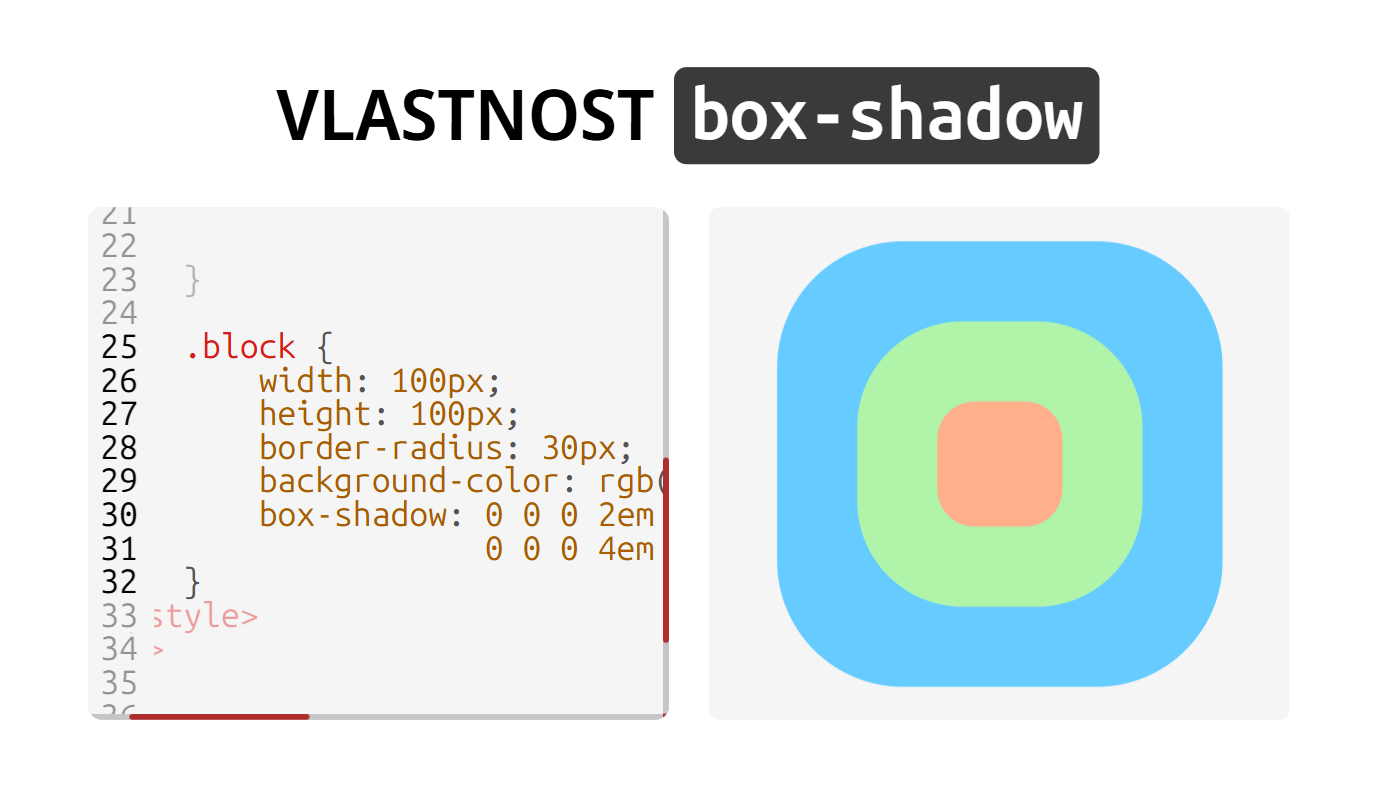
\includegraphics[width=0.9\linewidth]{media/03_analyza/revealjs.png}
    \caption{RevealJS prezentace s rozdělením kódu a výsledku}\label{fig:analyza:revealjs-ukazka}
    {\medskip\small Z mnou vytvořené prezentace pro předmět Webové aplikace.} 
\end{figure}

\subsection{Beamer v \LaTeX}

Beamer je třída v sázecím systému \LaTeX, která se zaměřuje na vytváření snímkových prezentací.
Nejvíce je Beamer společně s \LaTeX~populární v akademickém prostředí, zejména z důvodu jednoduchého sázení matematických formulí a zápisu pomocí kódového jazyka, který leccos dovoluje. 

Zápis je ale zároveň to nejvíce nenáviděné na \LaTeX~\cite{latex_reddit}, a to zejména z důvodu kryptických kódových chyb a různých zastaralých zápisů.
Vygenerované prezentace jsou taktéž statické a nedá se v nich dělat jakákoliv interaktivita. 
Za částečnou interaktivitu jde počítat možnost generovat fragmenty snímků tak, že se na dalším zobrazí pouze následující část textu.
Ve výsledku se pro každý fragment do výsledného PDF vygeneruje další snímek.

Výhodou takovéto kódové generace je, že z jednoho zdrojového kódu -- pro prezentaci -- se často dají tvořit taktéž skripta, a to tím, že přidáváme takové bloky kódu, které se vykreslí právě v jednom nebo obou módech.
Další výhodou je řada knihoven, které již existují mnoho let, a které dovolují komplikované vizualizace a vykreslování.
Jedna z nich je například knihovna TikZ. 

\section{Aplikace na grafickou tvorbu}\label{text:analyza/grafika}

Tato sekce se zaměřuje na nástroje, které umožňují snadno a rychle vytvářet vizuálně atraktivní materiály, ať už jde o grafiky, ilustrace, uživatelská rozhraní či jiné kreativní prvky doplňující prezentace a vzdělávací materiály.

\subsection{Canva}\label{text:canva}

Canva je webová platforma pro rychlou a snadnou tvorbu grafických materiálů, jako jsou plakáty, letáky, sociální příspěvky či prezentace, s bohatou nabídkou šablon, fontů a grafických prvků~\cite{canva_website}. 
Hlavní výhody Canvy spočívají v intuitivním uživatelském rozhraní~\cite{canva_recenze}, které je možná až příliš jednoduché, obrovské knihovně předpřipravených šablon a prvků, možnosti \enquote{drag-and-drop} úprav a snadné integraci multimédií.

Díky cloudovému prostředí umožňuje Canva týmovou spolupráci~\cite{canva_live_help, canva_live_features}, sdílení souborů v reálném čase a přístup k materiálům odkudkoli, přičemž většina základních funkcí je dostupná zdarma. 

Nevýhodou může být omezenější možnost zcela individuálního designu u některých šablon, menší preciznost u specifických grafických úprav a u pokročilých funkcí potřeba placené verze Canva Pro. 
Přesto je Canva velmi oblíbená pro rychlou tvorbu vizuálně atraktivních materiálů i mezi pedagogy, kteří nepotřebují pokročilé znalosti grafických programů a chtějí rychle připravit poutavé grafické materiály či prezentace.
Čeští pedagogové mají program Canva k dispozici zdarma po ověření~\cite{canva_education}. Tento nástroj je mezi pedagogy velmi oceňován zejména právě pro jeho jednoduchost~\cite{canva_facebook}.

Canva má taktéž za svůj cíl vybudovat zodpovědnou firmu, a proto se zaměřují i na školení svých uživatelů, jak tvořit kvalitní grafické materiály.
Tyto materiály, respektive kurzy, jsou zcela zdarma a tématy se zaměřují od logotypů, plakátů až ke tvoření kvalitních studijních materiálů pro specifické předměty.


\subsection{Figma}\label{text:figma_popis}

Figma je profesionální online nástroj pro design a prototypování uživatelských rozhraní, který se v posledních letech stal standardem v oblasti webového a aplikačního designu~\cite{figma_website}. 
Nabízí vektorový grafický editor, možnost vytvářet interaktivní prototypy a sdílet je v reálném čase s kolegy, což výrazně usnadňuje spolupráci v týmech~\cite{figma_website}. 
Velkou předností Figmy je její cloudové prostředí, ve kterém se změny ukládají automaticky a každý člen týmu vidí okamžité aktualizace, což zjednodušuje proces zpětné vazby a revizí. 

Nevýhodou může být vyšší křivka učení pro uživatele neznalé profesionálních grafických nástrojů a nutnost stabilního připojení k internetu, aby bylo možné plně využít funkce Figmy. 
Přesto Figma představuje výkonný a flexibilní nástroj, který může pedagogům a školám pomoci při tvorbě interaktivních rozhraní pro studijní materiály, e-learningové platformy či jiné digitální vzdělávací projekty.
Podobným problémem je omezený neplacený režim, který hodně omezuje počet a velikost projektů a to včetně počtu současných editorů dokumentu.

Inspirativní částí Figmy jsou velmi pokročilé možnosti editoru, jako je například interaktivní prototypování.
To zahrnuje například možnosti přepínání komponent či jednotlivých rámců.
Velké pozitivum je i velké komunitní zapojení do prosperity aplikace pomocí tvorby komunitních rozšíření a šablon.

Figma se zaměřuje i na tvoření poznámek či pláten~\cite{figma_figjam} ve své dceřiné aplikaci FigJam.
Tento nástroj je postaven na stejném editoru, jako používá hlavní aplikace.
Podobně Figma dovoluje pomocí různých šablon i tvoření prezentací.
Tyto prezentace však postrádají řadu nepostradatelných funkcionalit, jako jsou například animační schopnosti a optimalizace na procházení snímky.

\section{Aplikace na tvorbu materiálů}\label{text:analyza/materialy}
% \todo{Celkově k tomuhle dopsat spoustu věcí}

Tato sekce představuje nástroje, jež umožňují připravovat a distribuovat výukové materiály v podobě interaktivních prezentací, kvízů, vizuálních map či jiných vzdělávacích formátů.
Tyto nástroje tedy mají velmi podobné cíle jako aplikace, která má vzniknout z téhle práce.
Hlavním cílem těchto aplikací je zefektivnit a zpestřit proces učení, zvýšit zapojení studentů a nabídnout pedagogům možnosti, jak obohatit svou výuku o moderní a atraktivní formy obsahu.

\subsection{Genially}

Genially\todo{sem citaci} je online platforma pro tvorbu interaktivních materiálů, prezentací, infografik a dalších multimediálních podkladů, které mohou publikum aktivně zapojit do obsahu.
Platforma je navržena s důrazem na jednoduchost použití, aby byla dostupná jak profesionálům, tak i laikům.

Jednou z klíčových vlastností Genially je možnost rychlého přidávání interaktivních prvků~\cite{genially}, jako jsou kvízy, hypertextové odkazy, animace a různorodý multimediální obsah. 
Tyto funkce nejen zvyšují zapojení studentů, ale také podněcují jejich motivaci k učení skrze aktivní interakci s obsahem. 
Tím se platforma stává nejen nástrojem pro prezentaci informací, ale také prostředkem pro výuku založenou na principu konstruktivistické pedagogiky~\cite{konstruktivismus}. 
% Konkrétní příklady interaktivních prvků zahrnují již zmíněné odkazy, kliknutí, řazení, kvízy, interaktivní aplikace uvnitř a mnoho dalšího.

Velkou předností Genially je jeho intuitivní rozhraní a široká škála připravených šablon.
Tyto šablony jsou navrženy s ohledem na vizuální atraktivitu a dynamiku, což umožňuje rychlou tvorbu obsahu bez nutnosti pokročilých grafických znalostí.
Platforma tak poskytuje tvůrcům nástroje, které by jinak vyžadovaly~\cite{genially} komplexní software a odborné znalosti.

Genially je však placená služba, což může představovat značnou překážku pro vzdělávací instituce a jednotlivce s omezenými finančními zdroji. 
Bezplatná verze nabízí pouze omezenou funkcionalitu a materiály vytvořené v rámci této verze obsahují vodoznak.
Dále je export obsahu možný pouze u placených tarifů, a to v různých formátech, jako jsou PDF nebo HTML. 
Tato omezení mohou snižovat flexibilitu uživatele, který by chtěl svůj obsah sdílet, archivovat offline a nebo celkově více plánovat výuku. 
Zároveň nelze provádět vlastní úpravy kódu ani integrovat komunitní rozšíření, což je omezující pro uživatele, kteří by potřebovali pokročilé nebo zcela unikátní funkce.

Je třeba zmínit, že Genially jako firma je formálně napojena na platformu Canva~\cite{genially}, viz kapitola \ref{text:canva}, a tyto dvě služby sdílejí základ vizuálního editoru. 
Tento aspekt zvyšuje celkovou kvalitu uživatelského zážitku, protože editor se vyznačuje vysokou přehledností a snadnou manipulací s obsahem. 
Z tohoto pohledu lze považovat Genially za nástroj, který efektivně staví na osvědčených principech uživatelského designu a zajišťuje širokou dostupnost profesionálních vizuálních standardů.

Na základě vlastních zkušeností jsem využil Genially pro tvorbu několika prezentací a vzdělávacích materiálů. 
Zatímco samotná tvorba byla rychlá a relativně bezproblémová, setkal jsem se s určitými nedostatky, které ztěžovaly optimální využití platformy. 
Jedná se o:

\begin{itemize}
    \item Omezenost obsahu, kdy počet různých prvků, které lze vložit do plátna, je opravdu malý a obecně se tím pádem vytvořené materiály hodí pouze na hodně obecné předměty. Pro informační technologie neobsahuje aplikace skoro nic vhodného.  
    \item Limitace \enquote{klávesnice}, kdy spousta věcí lze dělat pouze v uživatelském prostředí pomocí klikání. 
    \item Omezené možnosti exportu, jelikož hotové prezentace nelze jednoduše stáhnout ve formátu \texttt{PDF} nebo \texttt{PPTX} bez placené verze. To omezuje offline využití materiálů.  
    \item Pomalá odezva editoru u složitějších projektů, kdy větší množství objektů způsobuje zpomalení při úpravách a načítání.  
\end{itemize}

Problémy jsem měl i při prezentování vytvořených materiálů. 
Studenti měli taktéž problémy vytvořené \enquote{aplikace} používat. 
Sdílené materiály nemají moc intuitivní rozhraní a interaktivní prvky, které lze vložit, nemají moc dobrý uživatelský zážitek.

Na Genially jsem mezi českými učiteli nenašel moc objektivních hodnocení.
Od platformy Učíme online existují webináře a kurzy~\cite{genially_ucimeonline}, které celou aplikaci představují.
Podobně lze najít v různých komunitách na sociálních sítích i v nesouvisejících skupinách~\cite{canva_facebook} různé názory, které zejména zmiňují složitou tvorbu lekcí.

\subsection{Mentimeter}

Mentimeter je webová aplikace určená pro interaktivní zapojení publika prostřednictvím online hlasování, dotazníků, kvízů, slovních mraků, průzkumů a anket~\cite{mentimeter}. 
Umožňuje učitelům a přednášejícím získávat okamžitou zpětnou vazbu od studentů, což napomáhá identifikovat oblasti nepochopení, zvýšit míru interakce a podporovat aktivní účast na výuce. 

Velkou předností Mentimeteru je jeho uživatelská přívětivost, široká nabídka interaktivních formátů, kompatibilita s mobilními zařízeními a snadná integrace do výukových scénářů, přičemž výsledky lze ihned zobrazit na obrazovce. 
Vzhledem k tomu, že Mentimeter se zaměřuje zejména na interakci a aktivní zapojení publika, nikoliv na obsah samotný, nenabízí~\cite{mentimeter_review} mnoho grafických funkcí pro tvorbu složitých nebo vizuálně bohatých materiálů. 
Podobně vyučující uvádí problém s rozdělením odpovědí na jednotlivé studenty či s velmi omezenou neplacenou verzí.

Stejně jako Genially zde chybí komunitně tvořené rozšíření a detailní možnosti kódových úprav, avšak pokud je cílem zvýšit interaktivitu a okamžitou odezvu od studentů, Mentimeter tento úkol splní velmi dobře.

Mentimeter jsem aplikoval několikrát ve výuce a splnil to, co jsem očekával, a to, že se zvýšila interaktivita ve výukové skupině. 
Velkým problémem je opravdu to, že obsah nejde upravovat natolik, aby šlo vytvořit originální a graficky rozlišitelný obsah. 
V aplikaci taktéž velmi chybí grafické možnosti, na jednotlivé snímky lze vložit pouze jeden interaktivní prvek s jednotkami grafických variací.

\subsection{Prezi}

Prezi je prezentační nástroj, který se odlišuje od klasických lineárních prezentací svou nelineární strukturou.
Místo jednotlivých snímků pracuje Prezi s jedním velkým plátnem~\cite{prezi}, na němž lze rozmístit text, obrázky, videa a další obsah do logických celků, mezi kterými lze dynamicky přecházet pomocí pohyblivých či přibližovacích efektů.
Aplikace je tedy takovým velkým plátnem, v podstatě jednou myšlenkovou mapou.
To však omezuje její použití na pouze jeden konkrétní případ způsobu výuky -- obyčejné prezentace, plakáty a další materiály zde vypadají velmi zvláštně.

Hlavní předností Prezi je vizuální atraktivita, flexibilita v organizaci obsahu a neobvyklý způsob zobrazení témat, který může pomoci udržet pozornost posluchačů a lépe vyjádřit souvislosti mezi jednotlivými informacemi. 

Nicméně Prezi nenabízí výrazně interaktivní prvky pro zapojení studentů, nepodporuje komunitně tvořená rozšíření a soustředí se především na propojení vytvořených témat společně s vizuálním aspektem prezentací, nikoliv na interakci či možnost programových úprav.

Prezi jsem se snažil použít, jejich editor je však velmi zvláštní a odbočuje od známých standardů \texttt{UI} a \texttt{UX}.
Prezi je taktéž placená aplikace a omezuje použití jakýchkoliv pokročilých obsahů, a tedy použití je bez toho prakticky nemožné a slouží spíše jako ukázka možností.

\section{Sumarizace knihoven a nástrojů}

V tabulce \ref{tab:porovnani_prezentaci} je sumarizovaná kapitola \ref{text:analyza/prezentace}, která se zaobírá různým softwarem na tvorbu prezentací.
Z tabulky vyplývá, že zatímco PowerPoint a Google Slides nabízí jednoduché a intuitivní použití, RevealJS a Beamer vyžadují znalosti kódování, ale umožňují větší flexibilitu. Největší rozdíly jsou v interaktivitě, přístupnosti a v dostupnosti pokročilých funkcí, přičemž žádný z těchto nástrojů není jednoznačně nejlepší pro všechny uživatele.


\begin{table*}[h!]
    \centering
    \resizebox{\textwidth}{!}{%
    \begin{tabular}{|p{2.3cm}||p{3cm}|p{2.5cm}|p{3cm}|p{3cm}|}
        \hline
        \textbf{Funkce} & \textbf{PowerPoint} & \textbf{Google Slides} & \textbf{RevealJS} & \textbf{Beamer} \\
        \hline        \hline
        Cena                & Placený & Zdarma & Zdarma & Zdarma \\\hline
        Prémiové funkcionality & Ano & Ano & Ano (Slides.com) & - \\\hline
        Přístupnost         & Desktop/Web & Web & Web & Lokální \\\hline
        Spolupráce          & Ano & Ano & Git/Cloud/IDE & Git/Cloud/IDE \\\hline
        Interaktivita       & Základní & Základní & Vysoká & Žádná \\\hline
        Šablony             & Bohaté & Bohaté & Flexibilní & Základní \\\hline
        % Podpora formátů     & PPTX &  & Webová &  \\\hline
        Používání           & Intuitivní & Intuitivní & Kódování HTML, CSS a JS & Obtížné \\\hline
        Unikátní vlastnosti & Integrace s Office & Cloudové ukládání & Interaktivní prvky & Možnost skript\\\hline 
    \end{tabular}%
    }
    \caption{Porovnání aplikací pro tvorbu prezentací}
    \label{tab:porovnani_prezentaci}
\end{table*}


V tabulce \ref{tab:porovnani_grafika} je sumarizovaná kapitola \ref{text:analyza/grafika}, která se zaobírá různým softwarem na tvorbu grafických materiálů, prezentací a návrhů aplikací.
Canva se vyznačuje jednoduchostí a rychlou tvorbou obsahu, zatímco Figma nabízí pokročilé nástroje a interaktivní prototypování, ale je náročnější na osvojení. Oba nástroje mají komunitní šablony, avšak Canva se zaměřuje spíše na rychlou grafickou úpravu, zatímco Figma cílí na UI/UX design s větší možností spolupráce v reálném čase.


\begin{table*}[h!]
    \centering
    \resizebox{\textwidth}{!}{%
    \begin{tabular}{|p{2.3cm}||p{6cm}|p{6cm}|}
        \hline
        \textbf{Funkce} & \textbf{Canva} & \textbf{Figma} \\
        \hline \hline
        Cena & Zdarma vs. Canva Pro & Zdarma vs. Figma Pro \\\hline
        Zaměření & Grafické materiály, prezentace & UI/UX design, prototypování \\\hline
        Přístupnost & Webová aplikace, mobilní verze & Webová aplikace, desktopová aplikace \\\hline
        Spolupráce & \multicolumn{2}{|c|}{Ano, v reálném čase} \\\hline
        Interaktivita & Omezená (základní animace) & Pokročilá (interaktivní prototypy) \\\hline
        Šablony & Bohatá knihovna & Šablony a komunitní rozšíření \\\hline
        Používání & Intuitivní, drag-and-drop & Náročnější, vektorový editor \\\hline
        Unikátní vlastnosti & Snadné použití, rychlá tvorba grafiky & Pokročilé nástroje, FigJam pro poznámky \\\hline
        Omezení & Méně přizpůsobitelné šablony, nutnost placené verze pro některé funkce & Vyšší křivka učení, omezený neplacený režim \\\hline
    \end{tabular}%
    }
    \caption{Porovnání aplikací na grafickou tvorbu}
    \label{tab:porovnani_grafika}
\end{table*}

V tabulce \ref{tab:porovnani_materialy} je sumarizovaná kapitola \ref{text:analyza/materialy}, která se zaobírá aplikacemi, které slouží k tvorbě materiálů.
Genially umožňuje tvorbu interaktivních vzdělávacích materiálů, ale omezuje uživatele placenými funkcemi a šablonovým systémem. Mentimeter je skvělý pro zapojení studentů do výuky prostřednictvím kvízů a hlasování, ale postrádá pokročilé grafické možnosti. Prezi nabízí inovativní způsob prezentování obsahu, ale kvůli své specifické struktuře není univerzálním řešením pro všechny výukové situace.


\begin{table*}[h!]
    \centering
    \resizebox{\textwidth}{!}{%
    \begin{tabular}{|p{2.3cm}||p{3.5cm}|p{3.5cm}|p{3.5cm}|p{3cm}|}
        \hline
        \textbf{Funkce} & \textbf{Genially} & \textbf{Mentimeter} & \textbf{Prezi} \\
        \hline \hline
        Cena & \multicolumn{3}{|c|}{Zdarma, placená verze s prémiovými funkcionality} \\\hline
        Zaměření & Interaktivní prezentace, infografiky & Interaktivní hlasování, kvízy & Prezentační software s nelineární strukturou \\\hline
        Přístupnost & Webová aplikace & Webová aplikace & Webová aplikace, desktopová verze \\\hline
        Interaktivita & Klikací prvky, kvízy, multimédia & Hlasování, dotazníky, slovní mraky & Zoom efekty, pohyblivé přechody \\\hline
        Šablony & Bohatá knihovna & Omezené varianty & Specifické pro Prezi formát \\\hline
        % Používání & Intuitivní & Snadné použití, rychlá odezva & Nestandardní ovládání, vyžaduje zvyk \\\hline
        Export materiálů & Pouze v placené verzi (PDF, HTML) & Omezené exportní možnosti & Placená verze nutná pro export offline \\\hline
        Unikátní vlastnosti & Kombinace vizuálních prvků a interaktivity & Okamžitá zpětná vazba od studentů & Nelineární prezentace, zoom efekt \\\hline
        Omezení & Omezená přizpůsobitelnost, placené funkce & Grafická jednoduchost, pouze jeden interaktivní prvek na slide & Malé možnosti interakce, zvláštní UX \\\hline
    \end{tabular}%
    }
    \caption{Porovnání aplikací pro tvorbu materiálů}
    \label{tab:porovnani_materialy}
\end{table*}

Z analýzy jednotlivých kategorií aplikací vyplývá, že neexistuje jeden nástroj, který by splňoval všechny potřeby uživatelů, což značně komplikuje výběr ideálního řešení. Každá aplikace se zaměřuje na specifickou oblast a přináší své výhody i omezení, což znamená, že uživatelé často musí kombinovat více nástrojů. 
Klíčovým problémem u většiny analyzovaných aplikací je závislost na placených verzích, omezená přizpůsobitelnost nebo nedostatek interaktivity.
Pro ideální nástroj by bylo zásadní nabídnout dostatečnou míru flexibility, široké komunitní rozšíření a otevřenost vůči uživatelským úpravám, což by umožnilo efektivnější a univerzálnější využití v různých vzdělávacích scénářích.

% \section{Interaktivní prvky}

% Interaktivní prvky jsou klíčovým nástrojem pro zlepšení zapojení uživatelů do výukového procesu a v této kapitole se zaměřím na to, co si pod nimi představit a jak je správně navrhnout.

% Použití interaktivity ve vzdělávání umožňuje studentům aktivně se podílet na výuce, což vede k lepšímu pochopení a zapamatování obsahu. 
% Existuje mnoho různých způsobů, jak lze interaktivitu integrovat do vzdělávacích nástrojů, přičemž každá metoda nabízí specifické výhody a vhodnost pro různé typy výuky.

% \subsection{Typy interaktivních prvků}

% Interaktivní prvky lze rozdělit do několika kategorií podle jejich funkce a způsobu využití:

% \begin{description}
%     \item[Hlasovací a anketní systémy] umožňují rychlou zpětnou vazbu od studentů a interaktivní zapojení do výuky. Používají se v reálném čase pro sběr odpovědí a jejich vizualizaci.
%     \item[Gamifikované kvízy] motivují studenty k soutěžení a učení se prostřednictvím herních prvků, jako jsou bodování, časové limity a různé formy zpětné vazby.
%     \item[Interaktivní prezentace] umožňují dynamické zobrazení obsahu s možností přímé manipulace, což usnadňuje pochopení složitějších témat.
%     \item[Virtuální simulace a modelování] poskytují realistické zkušenosti a experimentování v prostředí, kde by tradiční výuka byla obtížná nebo nemožná.
%     \item[Interaktivní pracovní listy] studentům umožňují samostatné procvičování a ověřování znalostí přímo v elektronické podobě.
%     \item[Kolaborativní nástroje] podporují spolupráci studentů na úkolech, sdílení nápadů a společné řešení problémů v reálném čase.
% \end{description}

% \subsection{Důležité aspekty při návrhu interaktivních prvků}

% Při tvorbě interaktivních prvků je nutné brát v úvahu několik důležitých aspektů:

% \begin{description}
%     \item[Uživatelská přívětivost] interaktivní prvky by měly být intuitivní a snadno ovladatelné, aby studenti mohli věnovat pozornost obsahu místo rozhraní.
%     \item[Didaktická efektivita] interaktivita by měla mít jasný vzdělávací účel a podporovat pochopení tématu, nikoli být jen vizuálně atraktivní.
%     \item[Technická dostupnost] je důležité zvážit kompatibilitu s různými zařízeními, operačními systémy a rychlost internetového připojení.
%     \item[Možnost zpětné vazby] ideální je, pokud prvky umožňují učiteli sledovat pokrok studentů a poskytnout jim personalizovanou zpětnou vazbu.
%     \item[Bezpečnost a ochrana soukromí] interaktivní nástroje by měly splňovat bezpečnostní standardy a chránit osobní údaje uživatelů.
% \end{description}

% \subsection{Využití interaktivních prvků ve výuce}

% Interaktivní prvky mají široké uplatnění v různých oblastech výuky. Jsou vhodné nejen pro klasickou školní výuku, ale také pro firemní školení, webináře nebo samostatné online kurzy. Jejich správné použití může výrazně zlepšit zapojení studentů, usnadnit pochopení abstraktních konceptů a zvýšit motivaci k učení. 

% Vhodná kombinace interaktivních prvků a tradičních výukových metod umožňuje vytvořit efektivní vzdělávací prostředí, které respektuje individuální potřeby studentů a podporuje aktivní učení.


\section{Způsoby vykreslování na webových stránkách}\label{text:vykreslovani}

Většina grafických aplikací potřebuje nějakým způsobem vykreslovat obsah programu.
Na webových stránkách jsme vykreslováním velmi omezeni.
Existují však různé alternativy zápisu a tvorby za pomocí různých prvků v HTML standardu.
Tyto způsoby v této kapitole rozeberu i s jejich plusy a mínusy.

\subsection{HTML prvky}\label{text:vykreslovani/html}

HTML je základní značkovací jazyk~\cite{uzayr2022frontend} pro tvorbu webových stránek. 
V rámci vykreslování obsahu na webu jsou k dispozici různé HTML prvky, které umožňují zobrazení statických i dynamických dat.
S pomocí CSS je možné tyto prvky skoro nelimitovaně~\cite{uzayr2022frontend} stylovat a pozicovat.

Použití tohoto způsobu je velmi jednoduché, protože je to v podstatě tvoření webové stránky.
Problém bývá s interaktivitou~\cite{uzayr2022frontend}, že i mimo tohle potřebuje s prvky pracovat a díky Document Object Model (DOM) je toto možné provést.
Kvůli častým změnám a závislostem proměnných na šablonách, resp. konkrétních prvků je často nutné vytvořit tzv. virtuální DOM.
Virtuální DOM tvoří a emuluje to, co dělá DOM, jen s tím, že program má nad celým vykreslováním, závislostmi celou kontrolu.
Virtuální DOM je klíčovou věcí pro skoro všechny moderní frameworky~\cite{uzayr2022frontend} na webových stránkách, jako React, Vue a tisíce dalších.

HTML, CSS, JS a (virtuální) DOM je poté možným způsobem, jak vykreslovat skoro jakýkoliv obsah na webové stránce a zároveň nad tím mít kompletní kontrolu.
Problémem bývá omezenost box-modelu a způsob pozicování, což může v některých případech limitovat flexibilitu při vytváření složitějších layoutů nebo interaktivních prvků. Box-model vychází z pevně dané šířky, výšky, okrajů, paddingu a okrajů okna pro prohlížeč, což může být komplikováno v případě, kdy je potřeba pracovat s dynamickým a variabilním obsahem. 
I když CSS nabízí pokročilé metody jako flexbox nebo grid, které značně zlepšují~\cite{uzayr2022frontend} flexibilitu layoutu, stále existují případy, kdy HTML prvky samy o sobě nestačí k dosažení požadovaného chování bez použití komplexního skriptování a dalších technologií.
Vykreslování je často pomalé s velkým počtem prvků díky (ne)optimalizacím prohlížečů.

Tento způsob používá velmi mnoho služeb a knihoven, jako ukázku uvádím například zmíněnou knihovnu RevealJS (viz kapitola \ref{text:revealjs}).

\subsection{Canvas}

Canvas je prvek z HTML~\cite{canvashtml5, uzayr2022frontend}, který je sémanticky a definičně určen k vykreslování komplexního grafického designu, her a podobných věcí.
Do Canvas se vykresluje pomocí JS (případně jiné jazyky, viz kapitola \ref{text:webassembly}) a to dovoluje měnit jednotlivé pixely, překreslovat je a tvořit animace.
Klasické módy Canvas jsou však omezené a často se aplikace rozhodnou používat nástavbovou knihovnu WebGL~\cite{canvashtml5}, která místo nekomplexního systému kreslení pixelů dovoluje komunikovat s GPU.
Dovoluje totiž definovat shadery~\cite{canvashtml5} pro GPU a spoustu dalších nastavení pro renderování obrazu.
Můžeme tedy tvořit velmi komplexní věci, optimalizovat to a webovou stránku ovládat jako jakýkoliv jiný obsah. 

Nevýhodou však může být složitost implementace~\cite{canvashtml5} a potřeba znalosti programování pro shadery.
V podstatě není nic dalšího definováno a i obyčejný okraj je nutné složitě naprogramovat.
Existují samozřejmě knihovny (např. ThreeJS) které pro nás definují~\cite{canvashtml5} shadery předem a dovolují další věci, jako např. načítání obrázků či modelů.
Navíc takto komplexní výpočty potřebují silnější zařízení, na kterých webová stránka běží.

I když je canvas sémanticky popsán~\cite{canvashtml5}, veškerý vykreslený obsah nikoliv a je tedy velmi těžké sémanticky určit, co se vlastně vykresluje.

Kvůli náročnosti tento způsob používá méně služeb, o zmíněných uvádím ukázku například Figma (viz kapitola~\ref{text:figma_popis}).
Jejich způsob vykreslování je velmi kvalitní a je vidět, že do aplikace investovali velmi mnoho zdrojů.
Jejím cílem je ale být grafický nástroj a přesnost všeho je pro jejich uživatele důležitá.

\subsection{SVG}

Scalable Vector Graphics (SVG) slouží k definování vektorových prvky~\cite{svg_css_html}, které se mohou jednoduše vykreslovat na webové stránce.
To dovoluje jednoduše používat daný vytvořený \enquote{obrázek} v jakémkoliv rozlišení.
Moderní SVG dovolují dovnitř jako prvek vkládat i rastrové obrázky a další cizí objekty~\cite{svg_css_html, uzayr2022frontend}, které se poté poměrně jednoduše vykreslují.

Veškeré prvky by se tedy pro vykreslování obsahu mohly definovat v jednom velkém SVG (kde by každá stránka či slide bylo jedno SVG), které by v sobě mělo jednotlivé prvky.

Mezi nevýhody tohoto systému je zejména problém s vykreslováním, protože rasterizace vektorového obrazu je drahá operace~\cite{svg_css_html}, a to zejména ve webovém prostředí.
Další omezení je i v tom, co s danými prvky poté jde dělat, protože tento způsob limituje to, co můžeme na dané prvky nastavit jako odchytávače události a respektive vůbec jaké události můžeme vkládat.
Hodně to ubírá na možné interaktivitě.
Dále se uvádějí~\cite{svg_css_html} nevýhody mezi kompatibilitou mezi prohlížeči.

Mezi výhody patří velké možnosti filtrů a definic, jednoduchý možný export a jednoduché transformace.
Tyto věci však umí i jiné varianty a nic navíc tento způsob nepřináší.

Toto vykreslování používá ze zmíněných služeb například Google služby, resp. Google Slides (viz kapitola~\ref{text:figma_popis}).

\section{Komunitní rozšíření}\label{text:community_plugins}

Cílem práce je vytvořit platformu, která bude podporovat komunitní rozšíření.
K tomu bude velmi důležité navrhnout, jak se toto rozšiřování bude realizovat.

V této sekci se podívám na to, jak komunitní rozšíření řeší jiné existující služby a knihovny.

\subsection{Google služby}

V kapitole~\ref{text:google_slides} jsem uvedl, že Google Slides integrují komunitní rozšíření -- úpravy platformy pomocí tzv. pluginů.
Tyto pluginy se používají tím, že uživatel v aplikaci nalezne tlačítko se správou rozšíření, ve kterém vybere rozšíření, které chce aktivovat.
Aktivací se spustí řada skriptů, se kterými poté samotná aplikace Google Slides komunikuje a zajišťuje danou funkcionalitu.

Tyto skripty mohou definovat~\cite{google_apps} například:

\begin{description}
    \item[API] Komunikovat s API Google Slides, tedy např. přidávat a modifikovat obsah jednotlivých snímku, přidávat snímky a nebo poskytnout přídavné okna s dalším obsahem.
    \item[Události] Zachytávat se na události a reagovat na ně skrz výše uvedené API.
    \item[Menu] Vytvořit speciální položky v navigaci, které budou dělat konkrétní změny.
\end{description}

Na spouštění skriptů uvnitř aplikace Google používá vlastní nástavbu jazyka JavaScript~\cite{google_apps}.
Tento jazyk a skripty v něm vytvořené se zásadně spouští na jejich serverech v emulátoru JavaScriptu tak, aby mohli jasně omezovat~\cite{google_apps} k čemu má daný skript práva. 
Mezi omezení patří např. omezení volání požadavku, přístup k tokenům a dalšímu.
Proto se nevolají skripty na klientské části, tedy není možné vytvořit emulátor, který poběží v bezpečném prostředí.
Alternativou v moderních prohlížečích je WebAssembly, které by něco takového mohlo dovolovat.
Tímto se budu zaobírat v kapitole~\ref{text:webassembly}.

Na internetu jsem hledal názory na tento způsob tvorby pluginů~\cite{google_apps_script_redit} a jeden z největších problémů, na které uživatelé píší hodnocení, je právě omezenost spouštěče kódu.
Vzhledem k tomu, že se pouští na serveru, je velmi limitována možnost měnit samotné HTML v prohlížeči a tedy i v prezentacích.
Pluginy jsou tedy velmi často omezené pouze na volání API a přidávání základních prvků, které ale nedovolují velké možnosti modifikace.
Možnosti jsou ale přesto velké, nevýhoda je, že je nutné mít vlastní server, umět jasně pracovat se zabezpečením Google a hlavně se chytře vyhnout, resp. přizpůsobit se těmto omezením.

Podobně taktéž fungují další služby od společnosti Google.
Většina aplikací poté specializuje své API, aby sloužilo konkrétní službě.
Jejich platforma na skripty -- Apps Script je stále stejná~\cite{google_apps_script_redit, google_apps} pro všechny služby.

\subsection{RevealJS}

RevealJS rozšíření, díky tomu, že správcem prezentace je přímo její programátor, nemusí až tak řešit.
Rozšíření se tvoří tak, že je vytvořen JS soubor, který se importuje při inicializaci prezentace pomocí RevealJS.
Tento kód si poté knihovna zaháčkuje jak je potřeba a plugin odpovídá na vše, co je potřeba.
Často knihovny dělají věci okolo tím, že vkládají obsah na stránku mimo vědomí knihovny, upravují jednotlivé funkce uvnitř a podobně.

Mezi ukázky pluginů patří například napojení knihovny \texttt{mermaidjs} pro vykreslování grafů, přiblížení při kliknutí nebo například načítání externího kódu ze souboru pro zobrazení v prezentaci.

Tyto rozšíření často nemají žádný důvod zneužít důvěry instalace a pokusit se napadnout prezentaci.
Často totiž není ani co za data vzít, protože jsou stránky hostované v nějakém hostingu, ve kterém se uživatel nepřihlašuje a nemá v něm žádná data.
To, co uživatel do prezentace nainstaluje, je zcela na něm.

K RevealJS patří služba Slides.com, která je postavena na dané knihovně od stejných autorů~\cite{slidescom}.
Tyto stránky již dovolují stránky sdílet, mají editor a vzhledem k tomu, že se již na stránce přihlašuje, sbírají se informace, je nutné, aby stránky omezily možná bezpečnostní rizika.
Proto platforma implementuje veškeré věci pomocí vlastních zabezpečených pluginů~\cite{slidescom} a jakékoliv věci ze třetích stran není možné používat.
Platforma ale implementuje řadu věcí a prezentace jsou použitelné.

\subsection{Figma}\label{text:figma}

Figma je velmi populární nástroj (viz kapitola \ref{text:figma}, který taktéž implementoval komunitní rozšíření~\cite{figma_website}.
Jejich přístup ke komunitnímu rozšíření je velmi veřejný a díky jejímu blogu~\cite{figma_plugins_blog} je vidět řadu důvodů kvůli zvážení každé možnosti.
Figma svými tzv. pluginy zajišťuje rozšiřitelnost platformy, resp. zjednodušení používání aplikace.
Mezi ukázky takových pluginů patří například různé možnosti vkládání ikon, šablon, ale i komplexní systémy na práci uvnitř editoru, jako hlasování v návrzích.

Pluginy se zejména zaměřují na práci v editoru, a proto některá rozhodnutí nejsou pro práci relevantní.
Při implementaci~\cite{figma_plugins_blog} se zaměřili na různé aspekty práce a způsoby spouštění nedůvěryhodného kódu, o kterých budu mluvit později.

Mezi její zvažované přístupy patřilo Iframe, Realms, WebAssembly a další.
Každý přístup měl pro a proti, proto se nakonec rozhodli z dvou užších možností -- Realms a WebAssembly -- přistoupit na Realms.
Jejich návrh platformy avšak dovoloval skoro bezpracné změnění způsobu volání kódu díky abstrakci.
To taktéž velmi rychle využili díky zranitelnosti Realms a i když volání WebAssembly nebylo lepší v celkovém porovnání, rozhodli se na něj přejít.
Jediná velká nevýhoda Realms je právě to, že daný kód běží ve stejném okně jako zbytek stránky a třeba i jeho zpomalení (nezáměrné i záměrné) může způsobit zaseknutí celé stránky.
Pro lepší bezpečnost je obecně počítat s tím, že se ze systému, kde je kód uzavřen, může kód dostat.

Mimo další platforma pro každou možnost zvažovala~\cite{figma_plugins_blog, figma_website} řadu kritérií a specifikací. 
Níže je takový seznam, který může pomoci rozhodnout mezi správným přístupem:

\begin{itemize}
    \item Bezpečnost takové implementace, rizika opuštění kontrolovaného prostředí.
    \item Jednoduchost psaní skriptů a i samotná implementace skriptů.
    \item Prostředky na spuštění takového kódu tak, aby to nebylo příliš náročné na zařízení.
    \item Kde spuštění probíhá, jak moc je možné systému věřit.
    \item Zpomalení spuštění skriptů a jeho reakce na události.
    \item Možnosti kódování a jeho jazyk.
\end{itemize}

\section{Spouštění nedůvěryhodného kódu}

Z kapitoly \ref{text:community_plugins} je očividné, že pro funkční a komplexní možnosti rozšíření jakékoliv aplikace je nutné vytvořit skriptovací platformu, která bude dovolovat spouštění nedůvěryhodného kódu.
Nedůvěryhodný kód jsou komunitní pluginy, které budou dovolovat programátorům upravovat stav aplikace a reagovat na možné události.

Ze stejné kapitoly vyšlo najevo, že čím více se toto spouštění omezuje, tím menší je využití dané platformy rozšíření.
Cílem této kapitoly je analyzovat možné způsoby spouštění nedůvěryhodného kódu a jejich výhody a nevýhody.

\subsection{Základní přístupy}

Uvnitř webových stránek díky podpoře JavaScriptu ve všech prohlížečích se lze bavit o základních přístupech k spouštění neověřeného kódu.
Jedná se o evaluaci (\texttt{eval}) a o domény (\texttt{realm}).

Přímá evaluace je funkce~\cite{eval} z JS, která dovoluje spustit jakýkoliv napsaný JS kód a získat z něj výsledek.
To dovoluje spuštění v podstatě jakéhokoliv skriptu v prohlížeči.
Problém v tomto přístupu je v tom, že nelze jakkoliv omezit k čemu má spuštěný kód přístup~\cite{eval, shadowrealms, figma_plugins_blog}.
Tedy má přístup ke všemu.
Omezení se dá pokusit vytvořit pomocí např. struktury \texttt{with}, která umí změnit kontext \texttt{this}.
To lze však velmi jednoduše obejít např. pomocí přístupu k prototype.
Tento způsob je tedy pro nedůvěryhodný kód nevhodný.

Alternativou k \texttt{eval} je využití \texttt{Realms}, což je mechanismus poskytovaný specifikací ECMAScript (prostřednictvím návrhu TC39)~\cite{shadowrealms_propsal}. 
\texttt{Realms} umožňují vytvořit izolovaný běhový kontext, kde spuštěný kód nemá přímý přístup k objektům a funkcím globálního kontextu hlavní aplikace~\cite{shadowrealms_propsal, shadowrealms}.
Každý Realm obsahuje svou vlastní kopii globálního objektu a základních vestavěných knihoven, což ztěžuje únik kódu mimo sandbox.
Přestože se jedná o bezpečnější variantu oproti \texttt{eval}, má \texttt{Realms} své omezení, například v podobě složitosti při komunikaci mezi hlavním a izolovaným kontextem. 
Problém mají taktéž s tím, že kód běží na jednom vlákně společně se zbytkem stránky a tak zásek v tomto kódu způsobí zaseknutí celé webové stránky.

Způsob pomocí \texttt{Realms} původně zvažoval a implementoval program Figma~\cite{figma_plugins_blog}.
V kapitole \ref{text:figma} je popsán postupný vývoj této platformy a to, jak se rozhodla z Realms, kvůli svým kritickým chybám, přejít na WebAssembly.

\subsection{Iframe}

Iframe je sémantický tag v HTML, který je určen pro vkládání stránky do stránky.
Iframe je velmi zabezpečený, protože pokud nejsou stránky ze stejné domény~\cite{iframe, figma_plugins_blog}, tak nemohou spolu komunikovat.
Vnější a ani vnitřní stránka tedy nemůže přečíst obsah a jakákoliv jiná data z druhé stránky.
Jediná možná komunikace je pomocí tzv. messagingu, kde si mezi sebou mohou stránky vyměňovat jednoduché textové zprávy.

Iframe má taktéž kvůli zabezpečení tzv. nulový (\texttt{null}) origin pro CORS~\cite{iframe, figma_plugins_blog}.
To omezuje, resp. neguje, nastavení webových stránek pro ochranu uživatelů.
Zabezpečení je celkově ale velmi stabilní a to díky častým updatům prohlížečů.
Z iframe se v podstatě nedá utéct, ale samozřejmě existovaly funkční pokusy o prolomení, např. se jedná o~\cite{iframe_vuln}.
Jedná se ale obecně o velmi stabilní ochranu, které můžeme věřit kvůli skvělé práci skoro všech prohlížečů.

Iframe se nejčastěji používá na omezení nedůvěryhodného HTML kódu~\cite{iframe}.
Bez omezení by vložený kód z rozšíření mohl utéci z daného přiřazeného prvku a taktéž volat jakýkoliv kód jako stránka.
To by mohlo vést k získání cookies či jiných lokálních souborů a tedy ke kompromitaci dat.

Tento způsob se nehodí používat na obecné skriptování -- je totiž velmi závislé pouze na předávání dat mezi oknem a danou stránkou, což je velmi limitující.

\subsection{Spuštění v emulátoru}

Jednou z možností, jak bezpečně spouštět nedůvěryhodný kód, je jeho izolace v samostatném procesu. 
Tento přístup zajišťuje, že kód nemá přímý přístup ke zdrojům hlavní aplikace. 
Pro zvýšení bezpečnosti je nutné využít nástroj \texttt{chroot}, který omezuje přístup spuštěného procesu pouze na konkrétní adresářovou strukturu.

Existují specializované knihovny, jako například \texttt{vm2} nebo \texttt{isolated-vm} pro JS, které umožňují vytvoření izolovaných prostředí pro spouštění kódu. 
Tyto knihovny však nejsou univerzálně použitelné, zejména v prostředí webových prohlížečů, kde nejsou podporovány. 
Tím pádem nelze tento přístup nasadit v případech, kdy má být kód spuštěn přímo v uživatelském prohlížeči.

Navíc v minulosti existovaly zranitelnosti, které mohly umožnit obejití těchto omezení, což může vést ke kompromitaci aplikace.
A to je na serveru velmi nežádoucí.
Je proto nezbytné pravidelně aktualizovat používané knihovny a sledovat nové bezpečnostní postupy.

Hlavním problémem tohoto přístupu je komunikace mezi izolovaným procesem a hlavní aplikací. 
Vzhledem k oddělení prostředí je komunikace omezená na asynchronní předávání zpráv, což přináší zásadní omezení. 
Například skript nebo plugin spuštěný v tomto režimu nemůže v reálném čase ovlivňovat stránku, což znemožňuje implementaci dynamických interakcí, jako je přidání prvku na stránku po kliknutí. 
Implementace něčeho takového by měla velmi velké zpoždění, a to se pro prezentační program nehodí.

Alternativou k samostatným procesům je spuštění nedůvěryhodného kódu v kontejnerech, například pomocí Dockeru. 
Tento přístup poskytuje vyšší úroveň izolace~\cite{docker}, protože kontejnery mají vlastní virtuální prostředí a mohou být snadno omezeny v přístupu k hostitelskému systému.

Jedním z příkladů implementace tohoto přístupu je projekt Glot.io~\cite{glotio}, který umožňuje spouštění kódu různých programovacích jazyků v izolovaných kontejnerech. 
Kontejnery však trpí podobnými problémy jako samostatné procesy~\cite{glotio}, zejména v oblasti komunikace a výkonu. 

Kontejnery totiž přidávají režii, což může vést k výraznému zpomalení při spouštění kódu a komunikaci s hlavní aplikací. 
Pro některé scénáře, například interaktivní webové aplikace, je toto zpoždění nepřijatelné.

\subsection{WebAssembly}\label{text:webassembly}

WebAssembly je nový způsob spouštění bezpečného kódu na webové stránce.
WebAssembly spouští pseudo-assembly kód~\cite{webassembly}.
Toto prostředí je velmi omezené, protože běží v jiném prostředí než obyčejné stránky~\cite{webassembly, figma_plugins_blog}.
Dané programy bez konkrétní implementace nemají k dispozici DOM a v podstatě cokoliv spojené s prohlížečem.
WebAssembly je samozřejmě možné spouštět i mimo webový prohlížeč, např. na serveru či desktopu v běhových prostředích jako je Node.js či Deno~\cite{webassembly}.

Tento pseudo-assembly kód se dá vygenerovat v podstatě z jakéhokoliv jazyku, oficiálně jsou podporované základní jazyky jako například C++, C\#, Rust~\cite{webassembly} a mnoho dalších.
Spuštěný kód v prohlížeči či v běhovém prostředí může komunikovat s předem připravenými funkcemi~\cite{webassembly}, které mohou již prohlížeč, resp. webovou stránku, modifikovat.
Spuštěný kód může v lineární paměti ukládat všelijaké data, ze kterých poté webová stránka může číst či i zapisovat data.
Samotný kód totiž může pracovat jenom s číselnými hodnotami a často je nutné je konvertovat z interních do externích typů.

Nevýhodou WebAssembly je poměrně malý výkon~\cite{webassembly, figma_plugins_blog} a poměrně špatné možnosti debugování.

Pro skriptování je to vhodnou alternativou díky možnostem jazyků. 
Na druhou stranu je to taktéž velký problém, protože udržovat dokumentaci a funkční několik jazyků je přinejmenším pro účely této práce skoro nemožné.

Pokud bych se rozhodl používat tento způsob skriptování, musel bych se zaměřit pouze na jeden jazyk.
Nejlogičtější varianta na skriptování přídavných rozšíření by byl nějaký jazyk, který je již určen na skriptování.
Na webu pro většinu vývojářů bude jasná volba JavaScript.
Pro spojení mezi WebAssembly a JS zajišťuje např. knihovna QuickJS~\cite{quickjs}, AssemblyScript~\cite{assemblyscript} a další.

Tyto knihovny zabalují nějakou formu běhového prostředí (nejčastější je emscripten~\cite{assemblyscript, quickjs, figma_plugins_blog}, který například používá systém rozšíření ve Figma~\cite{figma_plugins_blog}) přes kterou poté kód spouští.
Tyto knihovny avšak nepotřebují řešit jen spouštění, ale je nutné taktéž řešit již zmíněné předávání (resp. konverze) dat~\cite{assemblyscript} mezi spuštěným programem, spouštěčem a programem v prohlížeči.

\section{Požadavky}

Požadavky určují očekávané vlastnosti~\cite{uml_2007} a chování budoucí aplikace. Dělí se na dvě hlavní kategorie: funkční a nefunkční požadavky. Jsou klíčové pro správný návrh aplikace, aby byla schopna splnit veškeré definované nároky.

\subsection{Funkční požadavky}\todo{vrátit se k tomuto a níže po dokončení aplikace, aby to reflektovalo co to umí}

Funkční požadavky vymezují konkrétní funkcionality~\cite{uml_2007}, které aplikace musí podporovat. Na těchto požadavcích jsou postaveny případy užití (viz kapitola~\ref{chapter:analyza/uzivatelskePripady}), jež specifikují, jak bude aplikace využívána. Přehled všech identifikovaných funkčních požadavků je uveden níže.

\begin{description}
    \item[F1 -- Uživatelé]
    Systém musí umožnit správu uživatelských účtů, včetně registrace, přihlášení a změny nastavení uživatele. Ke každému uživateli jsou vedeny různé informace, jako je nastavení a preference. Veškeré uživatelské účty mají stejné pravomoce.
    
    \item[F2 -- Materiály]
    Uživatel musí mít možnost prohlížet, vytvářet, upravovat, sdílet, mazat a spravovat materiály. Materiál je soubor dat, které se vykreslují v přehrávači (viz F3). Mohou obsahovat jednotlivé snímky. Snímky obsahují jednotlivé bloky, které reprezentují např. text, obrázek či pokročilý graf.
    
    \item[F3 -- Editor a přehrávač]
    Systém musí umožnit uživatelům vytvářet a upravovat materiály pomocí vestavěného editoru s podporou správy snímků, bloků a interaktivity.\todo{spolupráce, verzování?}
    
    \item[F4 -- Média]
    Uživatel musí mít možnost přidávat do materiálů různé typy médií, včetně obrázků a videí.
    
    \item[F5 -- Šablony]
    Uživatel musí mít možnost vytvářet a používat šablony pro efektivnější tvorbu materiálů. Šablony jsou předpřipravené materiály, které obsahují různé typy snímků, které lze opakovaně používat. 
    
    \item[F6 -- Rozšíření]
    Systém musí podporovat komunitní rozšíření pro rozšíření funkcionality editoru a přehrávače.
    Schválená rozšíření budou k dispozici přímo v aplikace pro instalaci kýmkoliv.
    
    \item[F7 -- Import/Export]
    Systém musí umožnit importování a exportování materiálů do a z různých formátů.
\end{description}




\subsection{Nefunkční požadavky}
Nefunkční požadavky~\cite{uml_2007} neurčují přímo funkčnost aplikace, ale stanovují podmínky, které zajistí její dlouhodobou udržitelnost a kvalitu. Přehled všech relevantních nefunkčních požadavků je uveden níže.


\begin{description}
    \item[N1 -- Výkon]
    Aplikace musí být schopna efektivně pracovat i s velkými materiály bez znatelného zpomalení.
    
    \item[N2 -- Webová aplikace]
    Výsledek musí být alespoň webová aplikace, která bude napsána ve validním HTML, CSS a JS.
    
    \item[N3 -- Bezpečnost]
    Uživatelé musí být chráněni proti neoprávněnému přístupu k jejich datům pomocí ověřovacích mechanismů.
    
    \item[N4 -- Škálovatelnost]
    Aplikace musí být navržena tak, aby zvládla velký počet uživatelů a jejich materiálů bez ztráty výkonu.
    
    \item[N5 -- Podpora jazyků]
    Systém musí podporovat více jazyků a umožňovat snadnou lokalizaci.
    
    \item[N6 -- Kompatibilita]
    Aplikace musí být přístupná z moderních webových prohlížečů a různých zařízení bez nutnosti instalace softwaru.
    
    \item[N7 -- Modularita]
    Editor musí být navržen modulárně tak, aby bylo možné snadno rozšiřovat jeho funkcionalitu pomocí komunity (vlastní bloky) ale i komunitních rozšíření.
    
    \item[N8 -- Responzivní design]
    Aplikace musí být optimalizovaná pro použití na různých typech zařízení, včetně mobilních telefonů a tabletů.
    
    \item[N9 -- Intuitivní uživatelské rozhraní]
    Rozhraní musí být navrženo s ohledem na použitelnost a jednoduchost, aby umožnilo snadnou práci s materiály.
\end{description}
\section{Případy užití}\label{chapter:analyza/uzivatelskePripady}

Tato kapitola slouží k definici typů uživatelů aplikace a toho, jak aplikaci budou používat.
Případy užití rozvinují funkční požadavky~\cite{uml_2007} tak, aby bylo zcela jasné, co cílená aplikace má umět a implementovat za funkcionality.

Uživatelé -- aktéři této aplikace se dají rozdělit do následujících popisných skupin:

\begin{description}
    \item[Nepřihlášený uživatel] Tedy někdo, kdo je na webové stránce, nemá k dispozici materiál k používání. Může se například přihlásit.
    \item[Přihlášený uživatel] Tedy někdo, kdo je přihlášen v aplikaci a chce v aplikaci používat -- například používat či tvořit materiály.
    \item[Tvůrce] Tedy někdo, kdo vytváří materiály a je přihlášen. Může se jednat o učitele ale i obyčejného uživatele. Jeho cílem je v aplikaci vytvořit prezentaci, plakát či cokoliv jiného. V aplikaci musí být přihlášen.
    \item[Čtenář] Tedy někdo, kdo přišel do této webové aplikace číst, resp. používat materiály, které vytvořil někdo jiný. Může být přihlášen i nepřihlášen.
\end{description}


\begin{figure}[ht!]
    \centering
    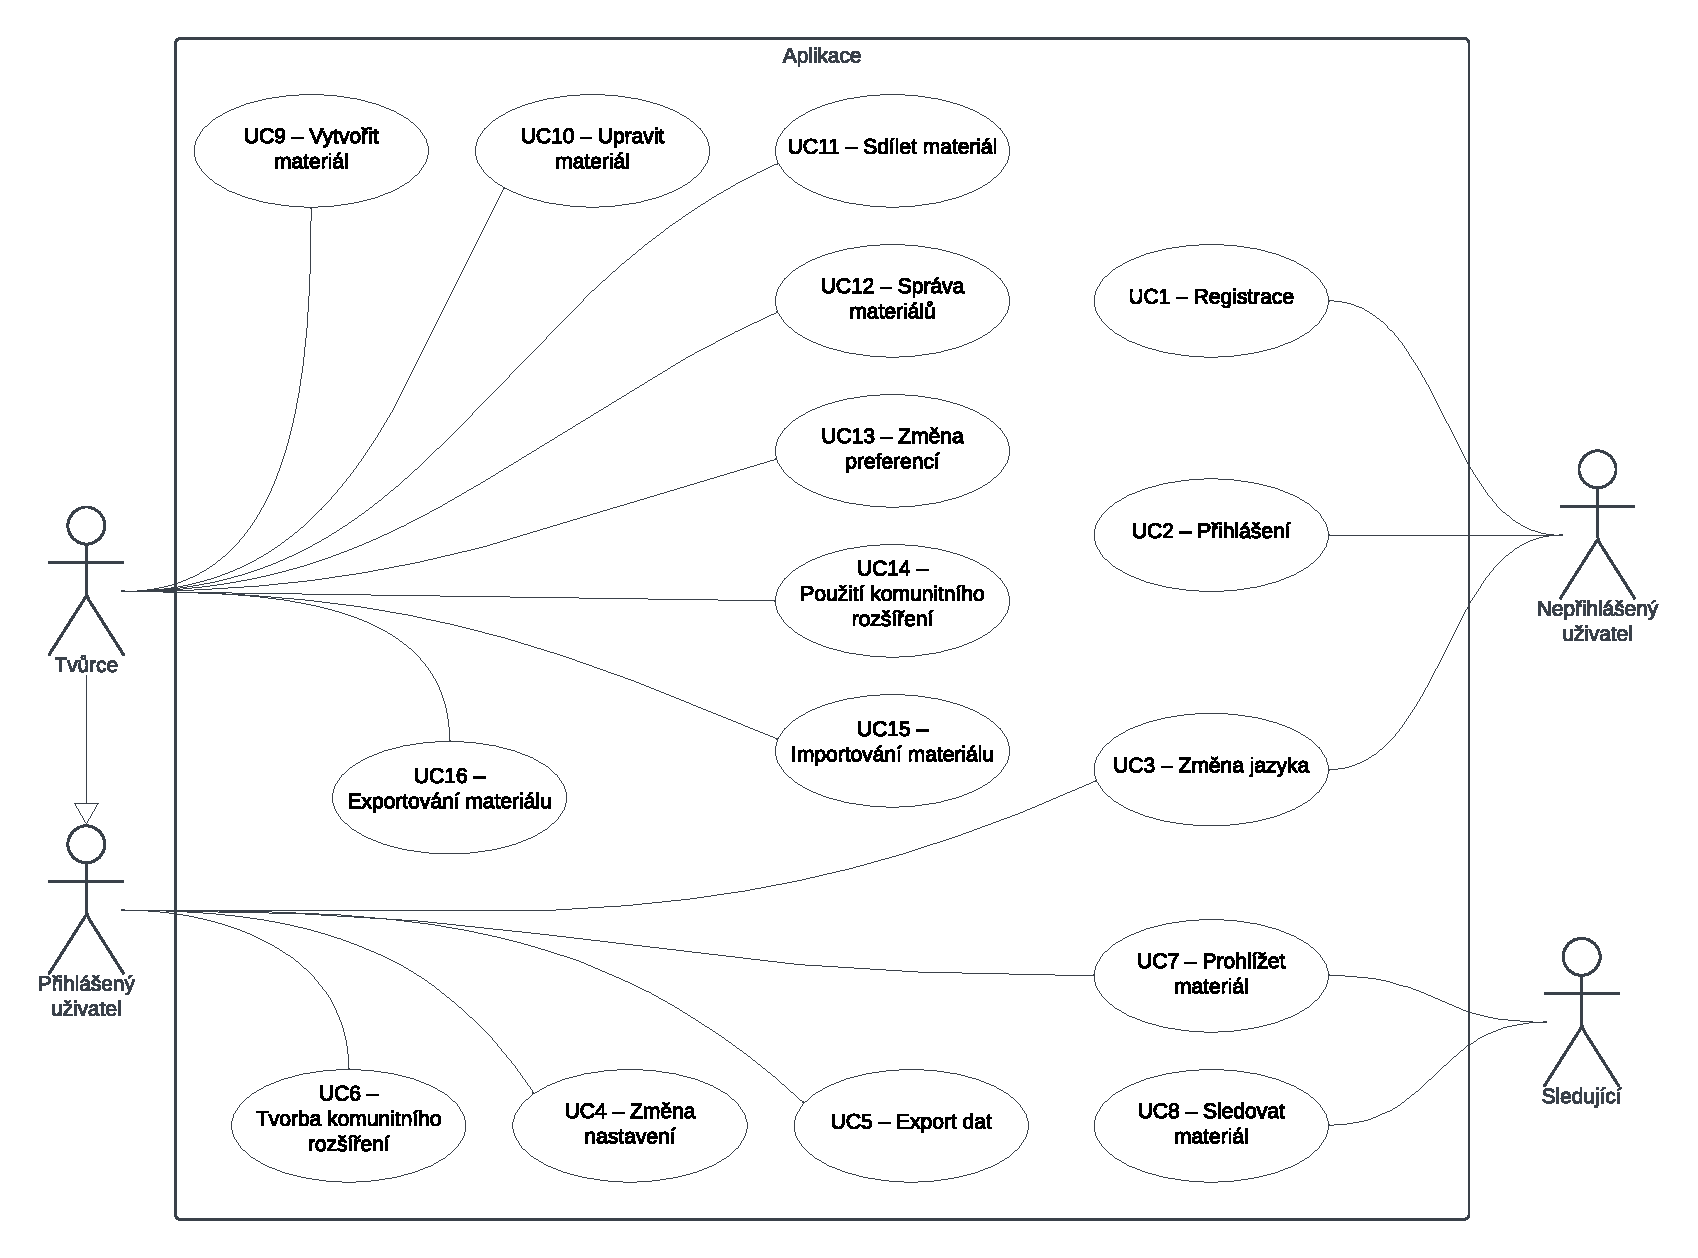
\includegraphics[width=1\textwidth]{media/03_analyza/uzivatelske_pripady.pdf}
    \caption{Diagram uživatelských případů}\label{fig:uzivatelskePripady}
\end{figure}

Níže jsou definovány všechny případy užití, které mají být implementovány ve výsledné aplikaci z této práce. Vztahy a propojení s jednotlivými aktéry jsou k dispozici na obrázku~\ref{fig:uzivatelskePripady}.

\begin{description}
    \item[UC1 -- Registrace]
    Uživatel se zaregistruje pomocí e-mailu a hesla. Po registraci je vyžadováno potvrzení e-mailové adresy prostřednictvím zaslaného ověřovacího odkazu.

    \item[UC2 -- Přihlášení]
    Uživatel se může přihlásit pomocí e-mailu a hesla. Alternativně lze použít ověření přes e-mail, kdy je na zadaný e-mail zaslán jednorázový přihlašovací kód.
    
    \item[UC3 -- Prohlížet materiál]
    Uživatel může procházet dostupné materiály. Musí mít možnost přecházet mezi jednotlivými snímky, interagovat s interaktivními prvky, přepnout na celou obrazovku, provádět pohyb v materiálu a další související akce.
    
    \item[UC4 -- Vytvořit materiál]
    Uživatel může vytvořit nový materiál buď od začátku, nebo duplikací existujícího materiálu.
    
    \item[UC5 -- Upravit materiál]
    Uživatel může provádět komplexní úpravy materiálu pomocí vestavěného editoru. Upravování je rozděleno do několika dílčích případů:
        
        \begin{description}
            \item[UC5.1 -- Správa snímků]
            Uživatel může přidávat více snímků, měnit jejich pořadí a upravovat jejich velikost.
            
            \item[UC5.2 -- Přidání bloku]
            Uživatel může přidávat jednotlivé bloky nebo skupiny bloků. Obsah může být čerpán z banky zdrojů, například GIFů nebo obrázků.
            
            \item[UC5.3 -- Úprava vlastností bloku]
            Uživatel může ručně měnit vlastnosti bloků, jejich zobrazení, grafiku a speficiké vlastnosti bloků. U interaktivních bloků lze definovat specifické akce, které se spustí při určité události (např. kliknutí, časovač, ...). Možné je také upravovat proměnné, nastavovat podmínky a další interaktivní chování.
            
            \item[UC5.4 -- Správa bloků]
            Uživatel může bloky označovat, kopírovat, mazat, přesouvat, seskupovat a provádět další operace.
            
            \item[UC5.5 -- Přidat média]
            Uživatel může nahrávat a vkládat vlastní obsah do prezentace.
            
            \item[UC5.6 -- Historie]
            Uživatel má přístup k historii úprav, může se pohybovat zpět a vpřed v provedených změnách.
        \end{description}
    
    \item[UC6 -- Sdílet materiál]
    Uživatel může nastavit viditelnost materiálu v různých režimech (nepřihlášený, pouze přihlášení uživatelé, soukromý). Lze definovat způsob procházení materiálu (automatický, ruční, pouze interaktivitou). Dále může povolit procházení materiálů jako plátna či jako prezentaci.
    
    \item[UC7 -- Správa materiálů]
    Uživatel může spravovat své materiály, zobrazit seznam, vyhledávat a provádět různé akce, včetně mazání materiálů.
    
    \item[UC8 -- Změna nastavení]
    Uživatel může měnit svá uživatelská nastavení, jako je heslo, e-mail a další osobní údaje.
    
    \item[UC9 -- Změna preferencí]
    Uživatel může upravovat nastavení editoru, způsob ukládání a způsob používání jednotlivých operací.
    
    \item[UC10 -- Změna jazyka]
    Uživatel může změnit jazyk aplikace. Aplikace se následně přepne do zvoleného jazyka. 
    
    \item[UC11 -- Použití šablon]
    Uživatel může vytvářet, upravovat a používat předdefinované šablony pro rychlejší tvorbu materiálů.

    \item[UC12 -- Použití komunitního rozšíření]
    Uživatel může instalovat a spravovat komunitní rozšíření, která umožňují přidávání nových funkcí do editoru.

    
    \item[UC13 -- Tvorba komunitního rozšíření]
    Uživatel může vytvářet vlastní komunitní rozšíření pro editor a přehrávač materiálů. Tyto rozšíření se píší ve skriptovacím jazyce a dovolují uživateli poslouchat různé akce, vytvářet bloky a upravovat je.
    
    \item[UC14 -- Importování materiálu]
    Uživatel může importovat externí soubory nebo formáty pro vytvoření materiálu.
    
    \item[UC15 -- Exportování materiálu]
    Uživatel může exportovat svůj materiál do různých formátů (např. PDF, obrázky, interaktivní formáty) pro sdílení a archivaci. Tato sdílení z důvodu nespolupracujících formátů budou velmi omezená svojí funkcionalitou a vzhledem.
\end{description}


Matice pokrytí určuje~\cite{uml_2007}, které funkční požadavky jsou nezbytné pro realizaci uživatelských případů. 
Zajišťuje kontrolu, zda každý funkční požadavek odpovídá alespoň jednomu uživatelskému případu a zda jsou pro každý uživatelský případ definovány všechny potřebné funkční požadavky. 
Pro tuto analýzu jsem sestavil matici pokrytí funkčních požadavků (viz tabulka~\ref{tabular:maticePokryti}).

\renewcommand{\c}{\checkmark}

\begin{table}[ht!]
\centering
\caption[Matice pokrytí funkčních požadavků]{~Matice pokrytí funkčních požadavků}\label{tabular:maticePokryti}
\begin{tabular}{l|c|c|c|c|c|c|c}
     ~         & F1 & F2 & F3 & F4 & F5 & F6 & F7 \\\hline\hline
     UC1       & \c &    &    &    &    &    &    \\\hline
     UC2       & \c &    &    &    &    &    &    \\\hline
     UC3       &    & \c & \c &    &    &    &    \\\hline
     UC4       & \c & \c &    &    &    &    &    \\\hline
     UC5       &    & \c & \c & \c & \c & \c &    \\\hline
     UC6       &    & \c & \c &    &    &    &    \\\hline
     UC7       & \c & \c &    &    &    &    &    \\\hline
     UC8       & \c &    &    &    &    &    &    \\\hline
     UC9       & \c &    & \c &    &    &    &    \\\hline
     UC10      & \c &    &    &    &    &    &    \\\hline
     UC11      &    & \c & \c &    & \c &    &    \\\hline
     UC12      & \c &    & \c &    &    & \c &    \\\hline
     UC13      & \c &    & \c &    &    & \c &    \\\hline
     UC14      & \c & \c &    & \c &    &    & \c \\\hline
     UC15      & \c & \c &    & \c &    &    & \c \\
\end{tabular}
\end{table}


\section{Doménový model}\label{text:analyza/datovymodel}

Pro lepší porozumění vztahům mezi jednotlivými prvky v aplikaci je nutné vytvořit doménový model. Tento model znázorňuje~\cite{uml_2007}, jak jsou entity vzájemně propojeny a jaká data uchovávají. Na základě doménového modelu lze následně navrhnout databázový model. Diagram doménového modelu je uveden na obrázku~\ref{fig:domenovyModel}. Níže jsou popsány klíčové entity tohoto modelu.

\begin{description}
    \item[Uživatel] 
    Entita reprezentující uživatele systému. Obsahuje informace jako jméno a příjmení, e-mailovou adresu, hashované heslo, stav aktivace, aktivační token, datum vytvoření účtu, datum posledního přihlášení a datum poslední změny hesla.

    \item[Žádost o přihlášení] 
    Entita uchovávající kód žádosti o přihlášení, jeho expiraci a stav použití, o které požádal konkrétní uživatel.
    
    \item[Preference] 
    Reprezentuje uživatelská nastavení editoru. Obsahuje možnosti ukládání, frekvenci ukládání, velikost historie a specifické funkce editoru. Vytváří se při vytvoření uživatele v aplikaci.

    \item[Soubor] 
    Entita popisující soubory nahrané do systému. Obsahuje mimo jiné název, MIME typ, velikost, typ úložiště a umístění souboru. Mohou se používat v konkrétních blocích materiálů.
    
    \item[Materiál] 
    Reprezentuje obsah vytvářený uživatelem. Obsahuje název, datum vytvoření a datum poslední úpravy. Obsahuje jednotlivé snímky.
    
    \item[Viditelnost] 
    Definuje viditelnost materiálu v systému pro ostatní uživatele. Je připojena k různým entitám pro správu jejich přístupnosti.
        
    \item[Procházení] 
    Nastavení pro procházení materiálu, zahrnuje způsob procházení a čas automatického přechodu mezi snímky.
    
    \item[Mód] 
    Určuje režim, ve kterém je materiál zobrazen nebo přehráván.
    
    \item[Snímek] 
    Každý materiál obsahuje snímky, které představují jednotlivé části obsahu. Entita obsahuje náhledový obrázek a pozici v rámci materiálu. Obsahuje taktéž data, které udávají nastavení snímku, např. velikost a šířku, a dále obsahuje bloky materiálu.
    
    \item[Blok] 
    Základní stavební prvek snímku. Obsahuje atributy jako typ, pozici, velikost, rotaci, přiřazenou skupinu, vrstvu, stav zamknutí a interaktivitu. Má další specifické vlastnosti v závislosti na konkrétním typu bloku. Například se může jednat o text, obrázek či komplexní blok pro zobrazení kódu.
\end{description}

\begin{figure}[ht!]
    \centering
    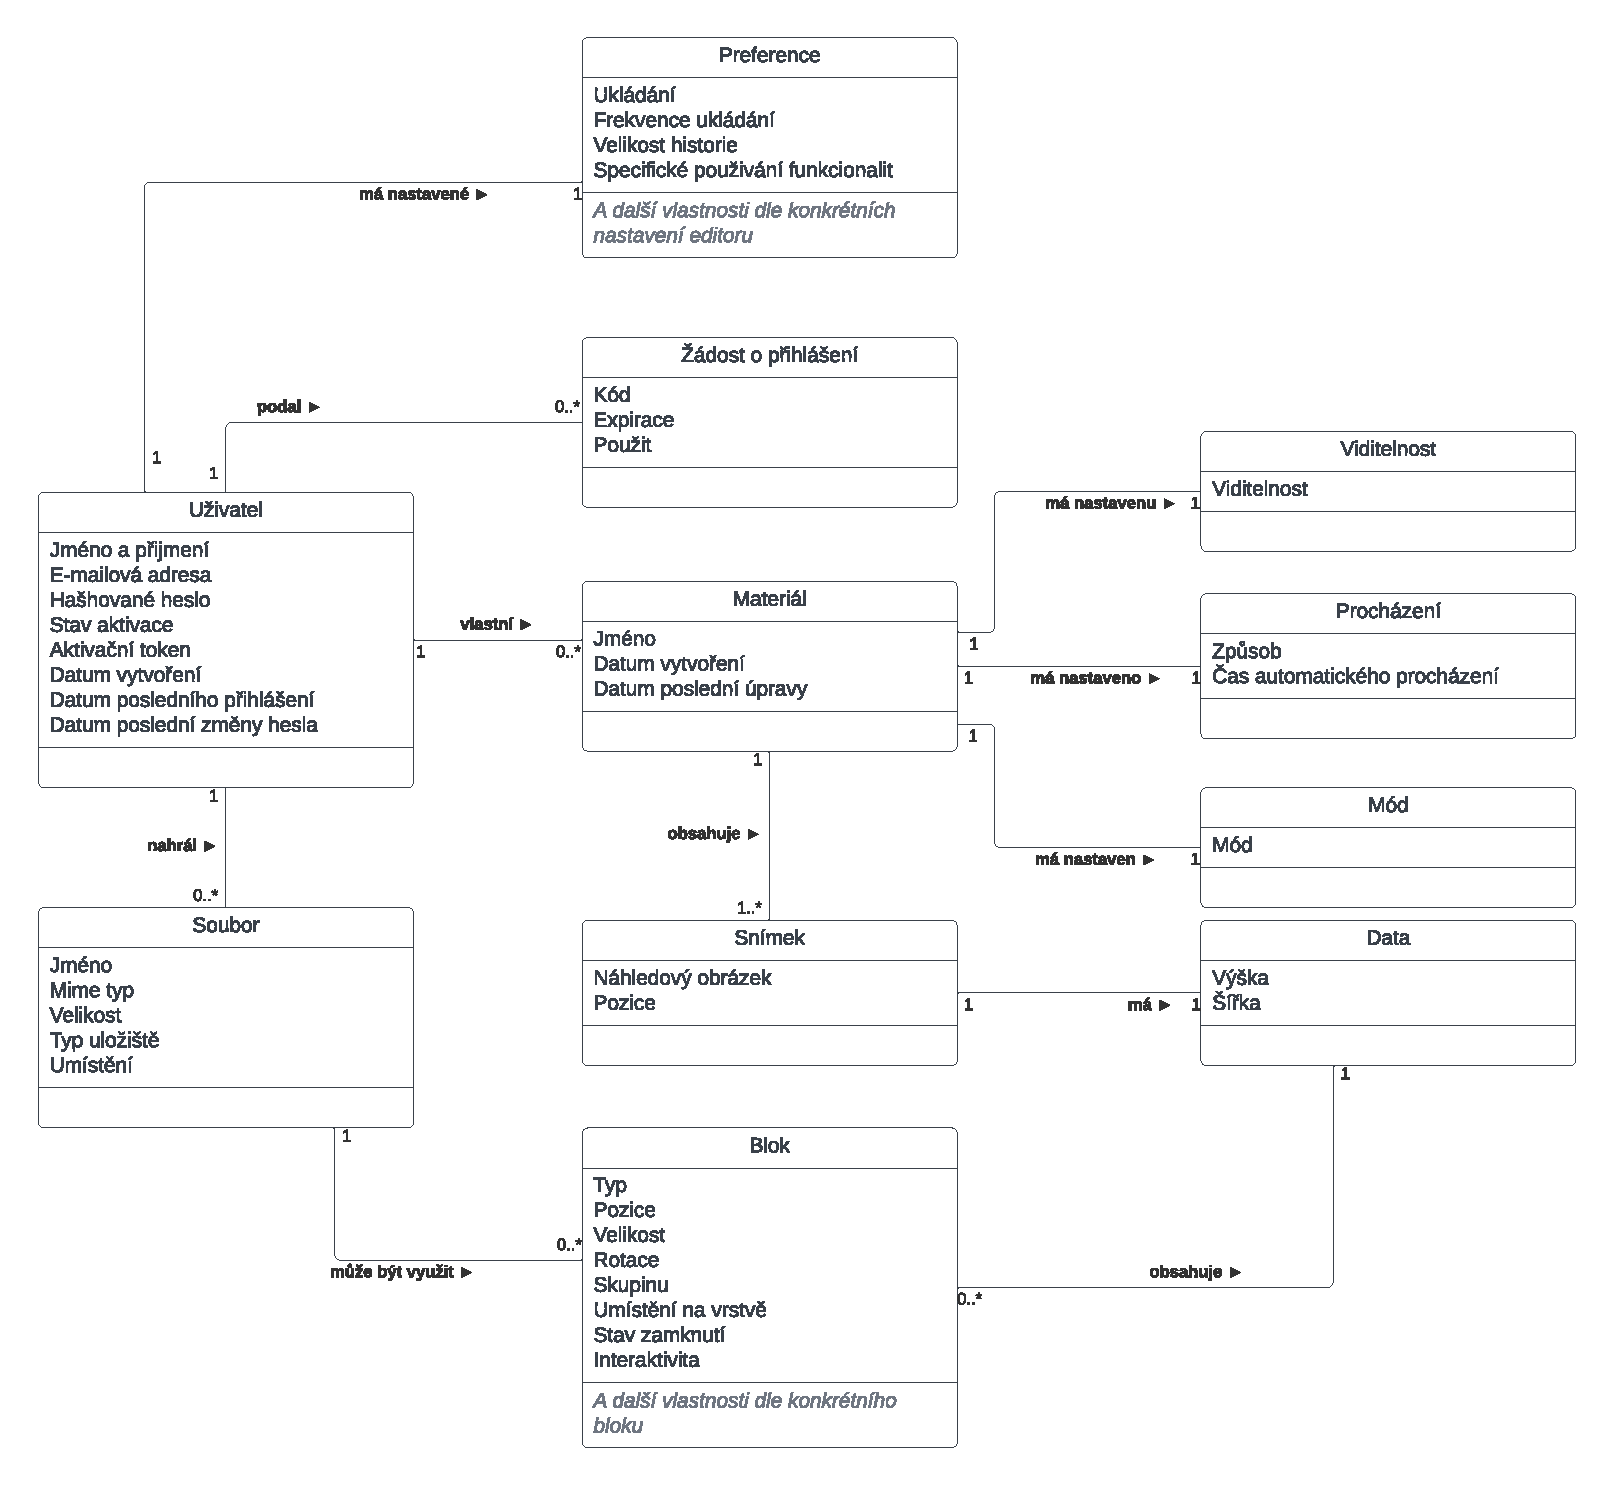
\includegraphics[width=1\textwidth]{media/03_analyza/domenovy_model.pdf}
    \caption{Diagram doménového modelu}\label{fig:domenovyModel}
\end{figure}\todo{předělat data a vztahy k nemu, BLOK > DATA nedávají smysl}
\chapter{Návrh}\label{text:navrh}

\begin{chapterabstract}
Tato kapitola představuje návrh architektury aplikace s důrazem na její modularitu, škálovatelnost a udržitelnost. 
Zabývá se rozvržením klientské a serverové části, volbou technologií a organizací kódu. 
Dále rozebírá klíčové prvky systému, jako je editor a přehrávač materiálů, možnosti komunitního rozšíření pomocí pluginů a bezpečnostní mechanismy pro ochranu uživatelských dat. 
Kapitola nabízí hlubší pohled na rozhodnutí, která ovlivní aktuální ale i budoucí vývoj platformy.
\end{chapterabstract}

\section{Architektura}

Návrh architektury je klíčový pro správný softwarový vývoj. 
Jeho cílem je vytvořit aplikaci a kód tak, aby byly snadno rozšiřitelné, přehledné a jednoduché k údržbě. 
Pokud je architektura špatně navržena, programátoři na ni často navazují a problémy se dále prohlubují.
Kód bývá často psán ve spěchu bez ohledu na budoucnost. 
Funkcionality lze implementovat různými způsoby, avšak důležité je myslet na možnost budoucího rozšíření a refaktorizace. 
Nepřehledný kód znesnadňuje jeho úpravy, údržbu i rozšiřování.

Základním prvkem architektury je definování odpovědností jednotlivých částí systému. 
Vzhledem k požadavku na webovou aplikaci byl zvolen model klient-server. 
Tento model je široce využíván, jelikož umožňuje vývoj multiplatformních aplikací, které lze používat na různých zařízeních. 
Klient může být vyvíjen nezávisle na serveru, přičemž je klíčové jasně definovat rozhraní pro vzájemnou komunikaci. 
V této aplikaci bude ke komunikaci používat zabezpečený protokol HTTPS.

Klientská část zpravidla představuje uživatelské prostředí běžící na zařízení uživatele a závisí na serveru. 
Serverová část zpracovává požadavky, odpovídá na ně a komunikuje s databází, externími službami nebo zajišťuje odesílání e-mailových zpráv. 
Následující části textu se věnují podrobnostem o struktuře jednotlivých komponent, použitých technologiích a způsobu jejich rozdělení. 
Diagram návrhu architektury je vyobrazen v obrázku~\ref{fig:architektura}.

% \begin{figure}[ht!]
%     \centering
%     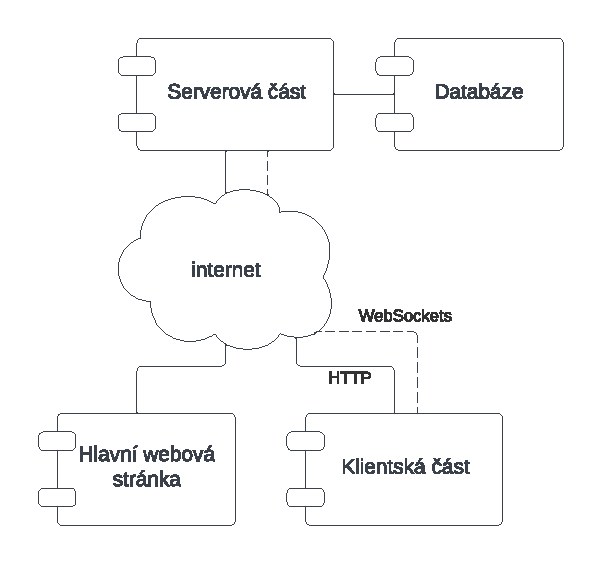
\includegraphics[width=0.85\textwidth]{chapters/navrh/architektura.pdf}
%     \caption{Diagram architektury aplikace}\label{fig:architektura}
% \end{figure}

\subsection{Klient}\label{text:navrh/klient}

Klientem celé aplikace bude webová stránka, ve které budou uživatelé vytvářet, přehrávat a procházet materiály. 
Obecně na této části budou uživatelé ovládat celou aplikaci.
Webová stránka je vhodná, protože to dovolí rychlejší přístup ke všem funkcionalitám bez nutnosti cokoliv instalovat.
Instalace taktéž není vhodná kvůli velkému počtu používání materiálů studenty, kterým by toto stahování mohlo přijít nevhodné.
Později by šlo z aplikace vytvořit nativní aplikaci na desktop či telefony pomocí enkapsulace webové stránky.

Tato část bude pomocí REST API komunikovat se serverovou částí za pomocí protokolu HTTP, ze které bude získávat veškerá potřebná data.
Restful API je ve zkratce takové API, které pracuje se zdroji jako takovými a dovoluje nad nimi volat klasické akce jako čtení, přidání, smazání a změnu (CRUD).
Mimo jiné definuje další standardizované chování, které by toto API mělo mít.
Tento způsob dovoluje tvořit tzv. \enquote{thick klienty}, které vysvětlím a zdůvodním později.

Klient tedy poběží ve webovém prohlížeči uživatele.
Díky tomu tedy musí být klient definován a stylován za pomocí HTML a CSS.
Kontrola samotné stránky musí být ve skriptovacím jazyce JavaScript.
Pro bezpečnější a udržitelnější kód však v této aplikaci použiji typovanou nástavbu TypeScript, která se kompiluje do čistého JavaScriptu.
Klient bude tvořen v myšlence \enquote{thick klienta}, tedy většinu funkcionalit by měl implementovat klient za pomocí dat a služeb, které dostane (má k dispozici) od serveru.
Toto dovoluje odlehčit server náročnými požadavky (překreslením HTML na serveru při každé akci a podobně) a soustředit se pouze na to důležité.
Klient taktéž bude moci být používán s menší závislostí na serveru a při správném nastavení například i dále dovolovat čtení, i když uživatel nebude připojen k internetové síti.
Nevýhodou je zátěž a dostupné funkcionality na zařízení, ve kterém webová stránka poběží, ale to by na dnešních zařízeních neměl být žádný problém.

V kapitole \ref{text:vykreslovani} zmiňuji různé způsoby vykreslování obsahu na webových stránkách.
I když je analýza směřována zejména na obsah, tak podobné myšlenky, zejména z kapitoly \ref{text:vykreslovani/html} lze aplikovat i na zbytek webových stránek.
Zjednodušeně, tvoření komplexních webových aplikací s mnohými funkcionalitami (což v tomto návrhu pro aplikaci plánuji) nelze dělat udržitelně pouze s \enquote{čistými} funkcionalitami HTML, CSS a JS.
Pro komplexní \enquote{thick klient} webovou aplikaci je nutné v moderním světě webového vývoje použít framework, který za nás bude řešit nejen uvedené:

\begin{itemize}
    \item Správu stavů aplikace a synchronizaci dat mezi komponentami.
    \item Efektivní aktualizaci a vykreslování uživatelského rozhraní.
    \item Modularizaci kódu pro lepší přehlednost a údržbu.
    \item Optimalizaci výkonu při práci s DOM (například virtualizaci seznamů).
    \item Zajištění kompatibility s různými zařízeními a prohlížeči.
    \item Možnost snadného rozšíření o další funkcionality pomocí dostupných knihoven a ekosystému.
    \item Automatizaci testování a zajištění stability kódu.
    % \item Podporu pro server-side rendering (SSR) nebo static site generation (SSG), pokud je to potřeba.
\end{itemize}

Jako webový framework pro klient použiji knihovnu Vue, která je známá\todo{zdroj} pro svoji jednoduchost, stabilitu a komunitou.
Dobrou alternativou by byl například React, avšak s ním nemám tak velké zkušenosti a z výběru z těchto dvou nedostanu žádné benefity na více.
Vue podporuje programování za pomocí TypeScript.

\subsubsection{Vrstvy a zodpovědnosti}

Klientská (a i serverová) část bude dále rozdělena na další části (tzv. vrstvy –- layers) pro zjednodušení celého systému zodpovědností v aplikaci.
To povede k přehlednějšímu kódu a jednodušším změnám v celé aplikaci.
V realizované aplikaci budou vrstvy pak dále děleny a bude vytvořena další abstrakce.
Níže jsou naplánované veškeré vrstvy pro klientskou část.

\begin{description}
    \item[Komponenty] Které zajišťuji unifikované chování pro často opakující se prvky na stránce tak, aby jejich tvorba byla co nejrychlejší a dovolovala přehlednější kód. Komunikují se stránkami pomocí dvoucestných vazeb či událostí.
    \item[Stránky] Které seskupují komponenty a vlastní funkcionality do jednotlivých stránek aplikace. Předávají komponentám data a určují jim, jak se mají chovat či zobrazovat.
    \item[Perzistence] Které jsou často nazývané ve webovém inženýrství jako obchody (stores), které globálně ukládají data pro celou aplikace, aby bylo jedno místo (či místa), kde je lze najít. Slouží k tomu, aby se o data nežádalo více, než je nutné (caching). Mohou dovolovat ukládat data zcela perzistentně i mezi načtením stránky pro rychlejší prvotní načtení. Komunikují se serverem pomocí další vrstvy.
    \item[Komunikace] Což zajišťuje komunikaci se serverem pomocí Restful API serveru. Určují a kontrolují jaká data od serveru přijdou, určují lokální rozhraní pro CRUD operace s danými zdroji a mapují je na lokální objekty.
\end{description}

\subsubsection{Editor a přehrávač}

Nejklíčovější částí klienta je editor a přehrávač materiálů, které budou uživatelé tvořit.
Editor i přehrávač jsou příliš komplexní a vzhledem k cíli práce vytvořit jednoduše rozšiřitelnou aplikaci (a to i díky komunitnímu rozšíření) a proto není vhodné pro tyto části webové aplikace použít zmíněný framework.
Rozšiřování frameworku by bylo velmi zvláštní a nebylo by to příliš intuitivní.
Hlavním problémem je však ztracení jakékoliv kontroly, jak a kdy se vykresluje daný obsah, co framework spravuje.
Z tohoto důvodu musí být takto komplexní komponenta, tedy editor a přehrávač, manuálně spravována.
Naštěstí framework Vue dovoluje označit část kódu jako spravovanou někým jiným a tento prvek nebude překreslovat, pokud se nezmění jeho závislost (tedy pokud mu to kód neoznámí). 
Takovéto fundamentální rozdělení taktéž dovolí, že editor se může velmi jednoduše přidat i do jiných projektů či komponent.

V pozdější kapitole \ref{text:navrh/editor_player} rozepíši, jak hodlám řešit to, jak se bude obsah zobrazovat v editoru a přehrávači, jak se bude upravovat, definovat a podobně.

\subsection{Server}\label{text:navrh/server}

Cílem serverové části je poskytovat data klientské části a to kvůli \enquote{thick klienta}. 
Tyto data bude server získávat z dalších služeb a zejména z databáze, ve které budou data perzistentně uložena.
O databázi budu rozepisovat v kapitole \ref{text:navrh/databaze}.
Mezi další služby bude patřit e-mailový server či různá další externí API třetích služeb (například na získávání obrázků a tak dále).

Poskytované API, což jsem zmínil v kapitole \ref{text:navrh/klient}, bude Restful a tedy bude pracovat jako se zdroji. 
Alternativní způsob designu API je například Simple Object Access Protocol (SOAP), který dovoluje volání akcí na serveru.
Standard REST API, jakožto moderní způsob komunikace, ukládá za povinnost takové věci API, které se slučují s navrhovanou aplikací.
SOAP by byl v tomto případě nevhodný a to zejména z důvodu, že server v tomto případě zejména slouží jakožto služba, která ukládá data.
Většina funkcionality v celém projektu je na klientské části, ve které se materiály vytváří a prezentují.

Server bude získávat data z URL adresy, těla a hlavičky požadavku.
Požadavky i odpovědi na a ze serveru budou komunikovat zejména v JavaScript Object Notation (JSON).
JSON je jednoduchý formát, který se jednoduše implementuje skoro v každém jazyce a je postaven na bázi seznamu klíčů a příslušných hodnot.
Hodnoty mají mnoho podporovaných datových typů.
Server by měl být však připraven na jakýkoliv formát dat.
Mělo by být možné velmi jednoduše změnit například na formát Extensible Markup Language (XML).

Serverová a klientská část by měly spolu sdílet rozhraní definující vstupní a výstupní data aplikace.
Těmto objektům se říká Data Transfer Object (DTO).
Tyto objekty dovolují jednoduše typovat data, které vstupují a vystupují do a respektive z REST API.

Některé endpointy a zdroje API musí být zabezpečené pomocí autorizace a autentizace. 
O zabezpečení budu mluvit v pozdější kapitole \ref{text:navrh/auth}.
Některé endpointy musí být limitované i rate-limitery, tedy že omezí počet volání daného endpointu pro konkrétního uživatele či globálně.
Jedná se např. o stránku s registrací.

Samotná serverová část bude tvořena v jazyce TS.
Volba TS je stejná jako v klientské části (viz kapitola \ref{text:navrh/klient}) a to tedy, že nutí programátora psát udržitelný kód, který je staticky typově kontrolován.

Implementace komunikačního uzlu je možná přes řadu způsobů a knihoven.
V JS, resp. TS ekosystému patří mezi nejoblíbenější backendový rámec knihovna Express.js (často taktéž Express).
Express je knihovna k vytvoření HTTP serveru, která dosahuje velmi úctyhodných rychlostí odpovědi a je velmi jednoduchá na pochopení.
Alternativní jako nejoblíbenější bývá\todo{zdroj} zmiňována knihovna Fastify.
Právě Express jsem se rozhodl použít díky své malé velikosti, komunitě a jeho velké stopě v ekosystému.
Express má řadu předpřipravených funkcionalit jako jsou routery, middleware a mnoho dalšího.

I přes to, že má Express mnoho připraveného, jeho používání bez jakékoliv nástavby je vhodné jen pro projekty, kde jde zejména o rychlost, a to i rychlost vývoje.
Pro udržitelnější servery je vhodné použít nějaký framework, který staví nad těmito knihovnami a dovoluje rychlejší zápis kontrolérů, modulů a služeb s pomocí Dependency Injection (DI).

Mezi nejznámější frameworky v JS ekosystému, které používají (nebo dovolují) Express, patří například NestJS či Koa.
Mezi nejvíce\todo{citace} oblíbené patří však NestJS a to zejména díky své velké komunitě, dokumentaci a rychlosti.
NestJS řeší vše dříve uvedené a mnoho dalšího.
Dovoluje rapidně tvořit udržitelné webové servery s HTTP API a podporuje řadu způsobů a knihoven návrhu.
Jedná se např. o passport, Mongo, Prisma, fronty úkolů, volání úloh, CORS, verzování API a mnoho dalšího.
Proto jsem se rozhodl NestJS s pomocí Express použít a to za pomoci TypeScriptu.

Server nejspíše bude používat i řadu dalších knihoven, například na odesílání e-mailů, jejich formátování a například na generování přihlašovacích tokenů pomocí JWT (viz kapitola \ref{text:navrh/auth}).

Výsledné API, které vznikne z této aplikace pokusí dodržovat vše, co uvádí standard REST.
To souvisí i s návrhem jednotlivých koncových bodů, které budou řádně uvádět stavové kódy, dodržovat metody komunikace a řadu dalšího.

\subsubsection{Vrstvy a zodpovědnosti}

I serverová část bude rozdělena do vrstev. 
Základ těchto vrstev je definován rovnou ve vybraném frameworku NestJS.
Avšak vrstev tam je definováno přespříliš, a proto hodlám používat jen část z nich.
V realizované aplikaci budou vrstvy pak dále děleny a bude vytvořena další abstrakce.
Níže jsou naplánované veškeré vrstvy pro serverovou část.

\begin{description}
    \item[Moduly] Ty sumarizují následující vrstvy do jednotlivých balíčků, se kterými se dá jednoduše pracovat. Definují co se má exportovat a importovat v rámci DI.
    \item[Služby] Ty sumarizují společné funkcionality do jednoo balíčku, aby se kód nemusel opakovat. Vztahují závislosti a agregují další služby a modely. Dají se sem počítat i tzv. Guardy, které kontrolují zda bude požadavek potvrzen a v aplikaci dále předáván do funkcí kontroleru.
    \item[Kontroléry] Ty tvoří REST API, volají funkce služeb, určují vstupní a výstupní data včetně návratových kódů.
    \item[Modely] Ty definují schéma databáze, respektive jednotlivých entit uvnitř.
\end{description}


\subsection{Databáze}\label{text:navrh/databaze}

Databázová část je zodpovědná za ukládání dat a poskytování rozhraní pro čtení a úpravu daných dat. 
V této části je potřeba databáze, respektive systém řízení báze dat (SŘBD).

Mezi zvažované možnosti jsem prvně přemýšlel o PostgreSQL a MongoDB.
Tyto dvě databáze poskytují základní spektrum pro databáze a to jsou~\cite{irena2015big, marek2018sql} SQL a NoSQL databáze. 
Aplikace jako celý cíl má stanovené to, že má být v budoucnu rozšiřitelná.
Je možné si představit, že tato aplikace bude v budoucnu ukládat velmi mnoho dat a bude potřeba, aby databázový stroj podporoval horizontální i vertikální škálování.
Podobně data, která budou v databázi uložena, nemají jasně stanovenou strukturu a obecně se bude jednat o velmi komplexní objekty.
V této aplikaci je lepší ztratit konzistenci dat, které např. MongoDB negarantuje (resp. je v módu \enquote{někdy bude konzistentní}~\cite{irena2015big}), důležitá je dostupnost a odolnost k přerušení.
I když budou na sebe data ukazovat (viz datový model v kapitole \ref{text:analyza/datovymodel}), jsou tyto propojení velmi triviální a spíše je vhodné dokumenty do sebe vnořovat.
Proto nevidím důvod na použití relační databáze a to i díky struktuře dat.

Alternativou s podobnými vlastnostmi~\cite{irena2015big} jako MongoDB je CouchDB a Firebase Firestore. 
CouchDB je dokumentová databáze, která využívá JSON pro ukládání dat, podporuje replikaci a je navržena pro distribuované systémy. 
Její hlavní výhodou je tzv. \enquote{multi-master} replikace, která umožňuje synchronizaci mezi více instancemi databáze. 
Firestore, jako součást ekosystému Firebase~\cite{firebase}, nabízí jednoduché škálování a real-time synchronizaci, což je výhodné pro aplikace s požadavky na okamžitou aktualizaci dat mezi uživateli. 
Nicméně, Firestore je úzce spjat s Google Cloud platformou a může být nákladnější v závislosti na objemu provozu a požadavcích na škálovatelnost. 
Vzhledem k těmto faktorům jsem se rozhodl zvolit MongoDB, která poskytuje dostatečnou flexibilitu pro strukturu dat i škálovatelnost bez závislosti na konkrétním poskytovateli cloudových služeb.

Díky výběru knihovny Nest (viz kapitola \ref{text:navrh/server}) je vhodné pro databázi použít takový driver, aby s ním i daná knihovna uměla pracovat.
V základním rozpoložení umí Nest pracovat mimo jiné s drivery (resp. ODM/ORM) Mongoose a Prisma~\cite{nest_database}.
S Mongoose mám velmi velké zkušenosti a používám ho i v projektech mimo Nest.
Prisma je na druhou stranu velmi populární nejen pro MongoDB, ale i pro ostatní databázové stroje.
Prisma má avšak velké problémy s MongoDB -- například se jedná o pomalejší dotazování\footnote{např. issue: \url{https://github.com/prisma/prisma/issues/16916}} či často je nutné velmi složitě nastavovat server~\cite{prisma_2025}.
Definice entit a jejich závislostí je taktéž velmi omezená.
Proto jsem se rozhodl použít s MongoDB právě knihovnu ODM mongoose.

\subsection{Databázové schéma}

Přestože návrh využívá nerelační databázi MongoDB, která nevyžaduje pevné schéma, je struktura dat vynucena pomocí ODM Mongoose na serveru.
Konzistenci dat tedy zajišťuje samotná aplikace při jejich zápisu a čtení. 
Pro vytvoření databázového schématu bylo nutné vycházet z doménového modelu a provedené analýzy z kapitoly~\ref{text:analyza/datovymodel}.

Navržené databázové schéma pracuje s relacemi, a proto jeho níže uvedená reprezentace není zcela přesná -- jde o hrubý návrh, kde jsou relace nahrazeny vazbami mezi jednotlivými dokumenty. 
V návrhu se rovněž nacházejí vlastnosti s datovými typy označenými otazníkem na konci, což signalizuje možnost absence dané hodnoty.
V kontextu MongoDB a JavaScriptu to znamená, že hodnota může být buď explicitně definovaná, nebo mít hodnotu \texttt{undefined}.

Entity v databázovém schématu odpovídají těm v doménovém modelu, avšak jejich názvy, atributy a další části byly přeloženy do angličtiny pro snadnější implementaci. 
Do návrhu byly doplněny další entity, dle provedeného návrhu aplikace, a také dekompozice vazeb typu \texttt{M:N}. 
Schéma je uvedeno v diagramu v obrázku \ref{fig:databazoveSchema}

Kompletní definice schématu jsou dostupné v kódové příloze ve složce \todo{složka}. 
Každá entita obsahuje validaci, která definuje platné hodnoty, povinné atributy, unikátnost či požadovanou délku.

\begin{figure}[ht!]
    \centering
    \includegraphics[width=1\textwidth]{chapters/navrh/databazoveSchema.pdf}
    \caption{Diagram databázového schématu}\label{fig:databazoveSchema}
\end{figure}

\section{Designový systém}

Uživatelské prostředí je klíčovou součástí každé aplikace, protože určuje, jak snadno a příjemně se s ní uživatelé budou schopni orientovat a pracovat. 
Je to nejen vizuální aspekt, ale i celková interakce mezi uživatelem a aplikací. Kvalitně navržené uživatelské prostředí může zlepšit uživatelský zážitek a zvýšit efektivitu používání aplikace.

Při návrhu aplikace je dobré si dopředu rozhodnout, jak bude uživatelské prostředí vypadat, aby uživatelský zážitek z celé aplikace byl co nejlepší. 
To zahrnuje nejen grafickou podobu, ale i logické uspořádání jednotlivých prvků, navigaci a celkovou ergonomii rozhraní.

Uživatelské prostředí lze rozdělit do dvou částí -- samotný designový návrh a technickou implementaci. 
V podstatě se jedná o komplexní designový systém. Ten určuje, jaké komponenty aplikace obsahuje, jak vypadají, jaké mají parametry, ale hlavně jak spolu navzájem interagují. 
Jako komponenty si lze představit tlačítka, vstupní pole, záložky a další, ale i jejich stav, například zda jsou vypnuté, zda vypadají speciálně, jejich pozice a mnoho dalšího.

Mezi známé designové systémy patří například Material Design od společnosti Google, který se používá nejen v Google aplikacích a systémech. 
Dále se používají například Apple Human Interface Guidelines, které jsou určeny pro aplikace v ekosystému iOS a macOS, nebo Fluent Design System od Microsoftu, který se používá především v aplikacích pro Windows.

CSS frameworky jsou v podstatě knihovny předpřipravených stylů a komponent, které usnadňují tvorbu konzistentního designu. 
Mezi známé CSS frameworky patří Bootstrap, který je jedním z nejpopulárnějších frameworků díky své jednoduchosti a široké komunitě, Tailwind CSS, který umožňuje větší flexibilitu při stylingu, nebo Bulma, který je založen na flexboxu a poskytuje moderní a elegantní vzhled.

Designové systémy a CSS frameworky jsou velmi dobrým nástrojem, který usnadní zejména vývojářům čas s vymýšlením prvků a designu, ale i zejména s funkcionalitou jednotlivých komponent. 
Problémem bývá ale to, že upravovat design těchto komponent a celkovou interakci mezi nimi je skoro nemožné. 
Proto často dovolují pouze změnit základní styly a třeba barvy jednotlivých stavů. 
Stránky, které používají stejné designové systémy, často vypadají identicky, a například v případě Google (při dodržení všeho uvedeného) si spousta uživatelů může myslet, že daná aplikace je přímo od nich. 
Tyto systémy se často hodí na nástroje a aplikace pro dané platformy.
Pro odlišení mezi konkurencí je skoro nezbytné si vytvořit vlastní systém, design a přemýšlet nad tím, aby si uživatelé stránku zapamatovali. 
To souvisí s designovou identitou a všechny pojmy se tímto propojují.

Designové systémy často mají předpřipravené komponenty pro různá prostředí. 
Například Material Design je implementován pro framework Vue (který jsem vybral v kapitole \ref{text:navrh/klient}) v různých knihovnách, mezi nejznámější patří například Vuetify či Quasar.

Výsledná aplikace je sice nástroj, ale reálně by měla být použita a být něco nového. 
Chtěl bych, aby aplikaci ihned kdokoliv poznal. 
Proto jsem se rozhodl nepoužívat žádný předpřipravený designový systém a vytvořit pro tuto aplikaci speciální, který bude plně odpovídat požadavkům a unikátně reflektovat její funkčnost a estetiku.

\subsection{Komponenty a styly}\label{text:navrh/desgin/komponenty}

Designový systém budu zakládat na komponentách a jejich interakcích.
Jednotlivým komponentám, ale i celé stránce, budu implementovat design.

Ve své bakalářské práci~\cite{cajthaml_bp} ale i v jiných projektech jsem implementoval řadu designových systémů.
Dle mého názoru je důležité si rozhodnout zejména o typech komponent, které se budou využívat.

Níže jsou uvedeny komponenty a jejich krátký popis, které bude zajisté nutné ve výsledné práci používat.
Celým seznamem se inspiruji zejména z již existujících projektů.
Plánuji taktéž použít část kódu z již vytvořených komponent, které jsem vytvořil.
Nějaké i z bakalářské práce, kterou jsem dále upravoval dle potřeb evoluce daného studijního informačního portálu. 

\begin{description} 
    \item[Upozornění] Slouží k upozornění uživatele na nějaký speciální stav – například chybu či varování. 
    \item[Tlačítko] K interakci s částmi aplikace, umožňuje akce, přesměrování a vizualizaci. 
    \item[Rozdělovač] Odděluje obsahové sekce pro lepší přehlednost. 
    \item[Dialog] Zobrazí modální okno pro potvrzení, zadání nebo informaci. 
    \item[Karta] Umožňuje organizaci obsahu do vizuálně oddělených bloků. 
    \item[Seznam] Strukturované zobrazení prvků pro snadnou orientaci. 
    \item[Záložky] Přepínání mezi různými sekcemi bez změny stránky. 
    \item[Stránkování] Rozděluje obsah na více stran pro lepší navigaci. 
    \item[Navigace] Umožňuje pohyb mezi různými částmi aplikace. 
    \item[Formulář] Sběr a odesílání dat od uživatele. 
    \item[Vstupní pole] Umožňuje zadání textových nebo číselných hodnot. Taktéž výběr z možností.
\end{description}

Mezi další základní styly, které bude nutné implementovat, patří:

\begin{itemize}
    \item Typografii a různé zvýrazňovací prvky.
    \item Grid systém pro rozdělení stránky do jednotlivých sloupců.
    \item Pomocné třídy na odsazení a základní rozložení, jako je například flexbox.
\end{itemize}

Komponenty se budou implementovat graficky, díky omezení a požadavkům na webovou stránku, pomocí HTML a CSS.
Funkčnost budu tvořit za pomocí interaktivního frameworku Vue.

Pro jednoduché grafické úpravy barev, odsazení a celkovou konzistenci skrz celou aplikaci je nutné implementovat tyto hodnoty jako proměnné.
Je možné je definovat jako nativní CSS proměnné či v nějakém CSS preprocesoru, jako je například Syntactically awesome style sheets (Sass).
Obě možnosti by byly dobrým rozhodnutím pro budoucnost projektu a ze dřívějších zkušeností avšak musím pro proměnné použít nativní CSS proměnné.
Ty jednodušeji dovolují měnit hodnoty za běhu a zároveň i dědičnost mezi prvky, což vytvoří systém, který reaguje na požadavky aplikace.
To taktéž dovolí vytvořit systém motivů, který bude měnit jednotlivé barvy v proměnných do předpřipravených stylů, které bude moci uživatel vybírat.

Přesto hodlám metajazyk Sass v práci používat, protože dovoluje například jednodušší vnořování jednotlivých selektorů či prosté cykly pro tvoření komplexních názvů, pro pomocné třídy.
Sass je nutné kompilovat, naštěstí to řeší rovnou spojení Vite společně s Vue za pomocí knihovny \texttt{sass}.

Styly budu psát přímo ke komponentám a pomocné třídy do globálních souborů, které budou vždy načteny.

Responzivitu komponent budu řešit jednotlivě a všechny pomocné třídy budou mít podpůrné třídy nebo automaticky nastavenou responzivitu.
Responzivita bude fungovat na tzv. breakpoint (či zlomové body) mechaniku.
To zajišťuje, že stránka je responzivní vždy do určité šířky zařízení.
Na webové stránce těchto zlomových bodů bude několik, což dovoluje přizpůsobení na většinu zařízení.
Na obrovských (širokoúhlých) monitorech se stránka umístí doprostřed obrazovky a více se neadaptuje.
Stránka bude responzivní na výšku automaticky díky nepoužívání relativních jednotek vůči výšce.

\subsection{Návrhové obrazovky}

Wireframy (také označované jako návrhové obrazovky) slouží k rychlému náhledu uspořádání prvků a obsahu v připravované aplikaci. 
Oproti detailnějším prototypům či mockupům se u nich klade důraz především na pozici a význam prvků, nikoliv na finální grafické zpracování či prokliky mezi obrazovkami.

Vytváření návrhů pro tuto aplikaci probíhalo v nástroji Uizard2. 

Během práce jsem se inspiroval zejména svými již dříve vytvořenými uživatelskými prostředími a obecně z nástrojů, které jsem analyzoval v kapitolách \ref{text:analyza/prezentace}, \ref{text:analyza/grafika} a \ref{text:analyza/materialy}.

Během práce bylo možné ihned provádět úpravy na základě zpětné vazby od uživatelů a lépe tak vyladit přehlednost nebo ergonomii rozložení. 
Více o testování a zpětné vazbě při tvorbě aplikace je k dispozici v kapitole \ref{text:testovani}.
Každá z vytvořených obrazovek proto odráží aktuální požadavky na funkčnost i strukturu aplikace.


Celkem vzniklo X návrhových obrazovek, jejichž ukázky jsou uvedeny v obrázcích Y a Z, zatímco úplný přehled všech návrhů lze nalézt v příloze \ref{appendix:navrhoveObrazovky}.
Mezi ně patří:

\begin{itemize}
    \item přihlášení, registraci
    \item TODO
\end{itemize}

\begin{figure}[ht!]
    \centering
    \includegraphics[width=0.9\textwidth]{chapters/navrh/navrhovaObrazovkaEditace.pdf}
    \caption{Návrhová obrazovka administrační části upozornění}\label{fig:navrhovaObrazovkaEditaceAdministrace}
\end{figure}


\section{Návrh editoru a přehrávače}\label{text:navrh/editor_player}

Při návrhu platformy bylo nutné definovat základní komponenty systému, které umožní tvorbu, editaci a následné přehrávání interaktivních výukových materiálů. 
Klíčovými prvky jsou bloky jako nejmenší jednotky obsahu, editor sloužící k jejich úpravám a přehrávač, který umožňuje interakci s uživateli.

\subsection{Bloky jako stavební prvky}

Základním konstrukčním prvkem v navrhovaném systému je blok. 
Každý blok představuje samostatnou jednotku obsahu, která může nabývat různých podob. 
V rámci návrhu je definována sada základních bloků, které lze kombinovat a upravovat podle potřeb uživatele.

Základní typy bloků mimo jiné zahrnují:

\begin{description}
    \item[Textové bloky] Které dovolují formátování textu, což zahrnuje velikosti, barvy, fonty a další.
    \item[Obrazové a multimediální bloky] Dovolují vkládání a manipulaci s obrázky, videi a dalším interaktivním obsahem
    \item[Tvarové bloky] Který umožňuje vložit předefinované tvary a jejich modifikaci.
    \item[HTML blok] Umožňuje skoro neomezeně rozšiřovat funkcionality prezentace pomocí psaní si vlastního HTML kódu, který se bezpečné vykreslí pomocí tagu iframe.
\end{description}

Bloky mohou být mezi sebou uspořádávány, transformovány a jejich vlastnosti lze dynamicky měnit. 
Každý blok může obsahovat specifické vlastnosti, která ovlivňují jeho chování a vizuální reprezentaci.
Mezi základní vlastnosti patří pozice, velikost, průhlednost, otočení a řada dalších.
Dále je možné blokům nastavit různé stavy, které mohou sloužit jako vodítka pro editor při jejich správě, jako je například zamezení transformace a podobně.
To se hodí, pokud bloky mají existovat pouze v nějakém určitém místě.

\subsection{Editor}

Editor slouží jako prostředí, ve kterém jsou výukové materiály vytvářeny a upravovány. 
Uživatelé zde mohou vkládat a přemisťovat bloky, nastavovat jejich vlastnosti a provádět transformace všeho obsahu.

Hlavní funkce editoru zahrnují:
\begin{description}
    \item[Práce s plátnem] Což dovoluje nastavovat velikost plátna, se kterým bude uživatel pracovat, dovoluje přibližovat a hýbat s ním.
    \item[Práce s bloky] Dovoluje již zmíněné transformace, změny vlastností, interakce a dalšího.
    \item[Správa pluginů] Která dovolí upravovat nainstalované a aktivní pluginy, jejich aktualizace a používání. Každý plugin v editoru bude mít své připravené místo na jeho ovládání, viz kapitola \ref{text:navrh/plugins}.
    \item[Vkládání obsahu] Umožňuje vkládat obsah z veřejných knihoven (fotobanky a další) ale taktéž z uživatelský zdrojů, do kterých si uživatel může nahrát vlastní obsah.
    \item[Nastavení] Dovolí nastavit viditelnost materiálů, způsob jeho průchodu a další.
    \item[Export] Dovolí uložit si kopie materiálu v různých formátech.
\end{description}

Editor informuje a reaguje na to, co dělá, například pomocí různých dialogů a vyskakovacích upozornění, aby umožnil intuitivní práci s materiály.

\subsection{Přehrávač}

Přehrávač je určen pro zobrazování a interakci s vytvořenými materiály. 
Uživatelé mohou obsah procházet, interagovat s prvky a využívat pokročilé možnosti zobrazení.

Funkce přehrávače zahrnují:

\begin{description}
    \item[Navigace] Přehrávač umožňuje procházet skrz snímky materiálu dle jeho nastavení. Tedy například průchod automaticky (časovačem), ručně či pouze pomocí interakce.
    \item[Pluginy] Dovolují upravovat a zobrazovat speciální obsah i mimo editor.
    \item[Interakce] Přehrávač dovoluje interagovat s prvky dle jejich nastavení.
    \item[Personalizace] Dovolují úpravu nastavení zobrazování podle preferencí uživatele.
\end{description}

Přehrávač je navržen tak, aby zajistil plynulou prezentaci obsahu a umožnil efektivní zapojení uživatelů do výukového procesu.

\subsection{Interakce v systému}

Interaktivita je klíčovou vlastností platformy.
Každý blok může obsahovat několik interaktivních nastavení, které reagují na různé akce. 

Mezi podporované interakce patří například časovače (po nějaké době, opakovaně) a různé uživatelské akce (kliknutí, najetí kurzoru) a mnoho dalšího. 

Po dané akci může interakce způsobit mnoho dalších akci, například se jedná o:

\begin{itemize}
    \item Upravit vlastnosti sebe i cizích bloků.
    \item Změnit snímek.
    \item Resetování bloku či jeho vlastnosti.
    \item Změnu hodnoty proměnné. 
\end{itemize}

Interakce se mohou spustit za nastavených určitých podmínek, jako je například čas na snímku, hodnoty proměnné a další.

Interakce jsou plně přizpůsobitelné a uživatelé mohou nastavit parametry, které určují jejich chování.
Lze taktéž nastavit animaci mezi jednotlivými stavy interakce.

\subsection{Kódový návrh}\todo{todo}

% - blok
%     - nejmensi jednotka v materialu
%     - muze byt cokoliv
%     - ze zakladu navrhuji vytvorit zakladni bloky jako:
%         - textové (práce s textem, velikosti, formatovani, barvy, fonty, ...) s pokrocilym editorem
%         - obrazek a dalsi multimedia
%         - tvary
%         - HTML
%     - bloky lze radit mezi sebou, upravovat, transformovat
%     - bloky maji vlastnosti, ktere ovlivnuji jak se chovani a vypadaji, kazdy blok muze mit jake chce
%     - ruzne stavy ve kterych jsou, *hinty* pro editor
    
% - editor - kde se edituji materialy
%     - instalují se pluginy (viz kapitola \ref{text:navrh/plugins})
%     - pohyb a celková transformace bloků
%     - pohyb a práce s plátnem
%     - vkládání dalšího obsahu a multimédií
%         - verejne banky
%         - vlastni nahravani obsahu

% - prehravace - kde se prehrava
%     - interakce s prvky
%     - dovoluje kresleni
%     - presouvani mezi snímky 
%     - pouzivaji se pluginy
%     - moznost ruzne nastavovat prochazeni

% - interakce
%     - kazdemu bloku muze byt nastavena interakce
%     - jedna se napriklad o:
%         - casove udalosti
%         - kliknuti
%         - najeti mysi
%         - a další
%     - na tyto udalosti blok muze reagovat:
%         - upravou sebe ci jinych bloku
%         - resetovanim bloku
%         - zmenu snimku
%         - zmeny hodnoty
%         - a další
%     - omezeni a nastaveni vsech hodnot, napriklad kdy se tato interakce muze vubec spustit
%     - animace pomoci interpolace hodnot

\section{Návrh komunitního rozšíření}\label{text:navrh/plugins}

Navrhovaná platforma bude podporovat komunitní rozšíření, což umožní uživatelům přizpůsobit si prostředí dle vlastních potřeb a vytvářet nové funkce nad základním jádrem aplikace.
Klíčovými aspekty tohoto rozšíření je jazyková kompatibilita, bezpečnost, registrace API a způsob distribuce pluginů.
Základní analýzou tohoto byla kapitola \ref{text:community_plugins}.

Jako hlavní programovací jazyk pro komunitní rozšíření byl zvolen JavaScript.
Tento jazyk byl vybrán pro svou jednoduchost, širokou adopci a kompatibilitu s webovým prostředím.
Skripty budou spouštěny pomocí knihovny QuickJS, která umožňuje běh JavaScriptu na straně klienta s minimalizovanými bezpečnostními riziky díky využítí WebAssembly.
Aby byla zajištěna integrace s editorem a přehrávačem platformy, bude vytvořeno API, které umožní pluginům komunikaci s těmito komponentami. 
Přímá abstrakce nad API nebude implementována, vzhledem k tomu, že zmenšení bezpečnosti QuickJS není pravděpodobné.
Pokud by se stala knihovna QuickJS nebezpečnou tak, že by z ni mohli jednotlivé rozšíření uniknout, budou pravděpodobně nefunkční všechna další jiná řešení.

Každý plugin bude sestávat z několika klíčových částí. 
Základem je manifest, který bude obsahovat základní informace o pluginu, jeho verzi a další nastavení. 
Další částí je samotný kód pluginu, který bude realizovat požadovanou funkcionalitu v přehrávači. 
Třetí část tvoří kód pro editaci v rámci editoru. 
V databázi platformy bude navíc uchovávána metadata, jako je název pluginu, jeho popis, informace o autorovi a jeho verze.

Systém verzování bude umožňovat udržení kompatibility s předchozími verzemi platformy. 
Nové verze pluginů budou vyžadovat aktualizovaný manifest, přičemž starší verze pluginů budou nadále funkční pro existující instalace. 
Uživatelé však nebudou moci instalovat starší verze pluginů, čímž se zajistí plynulá aktualizace celého ekosystému.
V rámci jedné instalace nebude možné mít aktivní více verzí jednoho pluginu současně.

Pro rozšíření funkcionality editoru i přehrávače bude možné registrovat API pro různé bloky a celý editor či plugin.
Editor bude umožňovat modifikaci velikosti, vytváření a úpravy jednotlivých bloků, zatímco přehrávač nabídne možnosti manipulace s přehrávaným obsahem, včetně navigace mezi snímky.
Mezi další API budou různé debugovací nástroje, posílání požadavků či třeba systém cache pro ukládání dočasných dat.
Dále bude pro rozšíření možné registrovat panely přímo do uživatelského rozhraní, což umožní hlubší integraci pluginů.
Panely budou implementovány s využitím iframe technologie, která zajistí izolaci kódu a zvýší bezpečnost systému.

Podobně bude vytvořen systém, kdy plugin bude moci vytvořit sám pro sebe určitý blok tak, že pouze on ho spravuje a vykresluje.
To dovoluje si ukládat speciální data a vytvořit řadu dalších funkcionalit.
Tyto bloky budou v podstatě již zmíněné HTML bloky, jen budou dovolovat ukládaní dalších dat, registraci vlastních vlastností a další věci.

Rozšíření budou moci oběma směry komunikovat jak s pluginy, tak i s jednotlivými bloky.
To dovolí řadu budoucích rozšíření, kdy například kliknutí v panelu vytvoří blok, který se může informovat plugin o tom, že se něco děje.

Bezpečnostní aspekty budou klíčovým prvkem návrhu.
Správné používání QuickJS je zásadní pro minimalizaci rizik spojených se spuštěním nedůvěryhodného kódu.
Komunikace mezi pluginy a hlavní aplikací bude co nejjednodušší, přičemž veškerá data budou podrobena validaci v každém použití.
Logování chyb a aktivit pluginů umožní lepší sledování a detekci potenciálních problémů.
Omezena bude také funkcionalita pluginů z hlediska síťové komunikace, zejména co se týče možnosti provádět HTTP požadavky (pomocí funkce \texttt{fetch}), čímž se zamezí neoprávněné komunikaci se servery třetích stran.
Uživatelé budou o speciálních povolení pluginů obeznámeni před instalací.

Pro podporu komunitního rozšíření bude nutné zajistit i dokumentaci a nástroje, které usnadní vývoj pluginů. 
Dokumentace bude pokrývat jak základy tvorby pluginů, tak možnosti rozšíření kódu samotné platformy. 
Důraz bude kladen na snadnost implementace a přístupnost pro širší komunitu vývojářů.
Nejvíce klíčové bude, aby pluginy měli jasně vytvořený systém typování, které dovolí kontrolu pluginu před během a pomocí IDE dovolí uživatelům prozkoumávat celé API.

% - základní analýza dle kapitoly \ref{text:community_plugins}
%     - jazykem bude JS, vzhledem k jednoduchosti a typingu
%     - spousteni pomoci quickjs, bezi u klienta
%     - vytvoreni API ktere bude dovolovat komunikovat s editorem/prehravacem
%     - nevyuzuji abstrakci nad api, protoze by to zpusobilo velmi velke zkompilovani tvorby
%     - pluginy na serveru, moznost pouzivani

% - pluginy se skladaji z:
%     - manifestu (nastaveni, verze)
%     - plugin kodu
%     - editor kodu
%     - v db dale ulozene info o: jmeno, description, autor
    
% - system releases
%     - novy kod, manifest
%     - stare verze pluginu (pro aktualni manifest verzi editoru) funguji
%     - stare verze nelze instalovat - uzivatel je musi aktualizovat
%     - dve verze nelze mit najednou
    
% - vytvoreni features, ruzne registrace API pro bloky
%     - komunikace podle daneho zamereni
%     - editor - velikost, bloky, vytvreni, jejich uprava
%     - prehravac - velikost, ovladani pozice slidu
%     - registrace panelu
%     - bloky primo pro pluginy, pomoci iframes, panely taktez
    
% - nutne myslet na bezpecnost
%     - spravne pouzivani quickjs
%     - komunikace stroha, dumpovani a validovani vsech hodnot
%     - logováni chyb a toho, co jaky plugin dela
%     - napriklad omezeni funkcionalit, komu muze delat fetch pozadavky

% - dalsi komunitni rozsireni:
%     - programovani tak, aby byla aplikace jednodusi
%     - vytvoreni dokumentace tvorby pluginu ale i rozsirovani samotneho kodu a moznosti
%     - jednoduche moznsoti pridavani novych typu bloku

\section{Autentizace a autorizace}\label{text:navrh/auth}

Autentizace je proces ověřování identity uživatele, tedy zajištění, že se daná osoba skutečně nachází v systému. 
Typickými metodami autentizace jsou přihlašování pomocí uživatelského jména a hesla, biometrické údaje nebo autentizace prostřednictvím třetích stran.

Autorizace naopak určuje, jaká oprávnění má autentizovaný uživatel v rámci systému.
Rozhoduje tedy o tom, ke kterým zdrojům má uživatel přístup a jak s nimi může nakládat.

\subsection{Autentizace}

V rámci této práce se autentizace soustředí na dvě základní metody přihlašování: kombinaci e-mailu a hesla a potvrzení pomocí odkazu zaslaného na e-mailovou adresu uživatele. 
Po úspěšné autentizaci se vygeneruje JWT (JSON Web Token), který slouží k ověřování uživatele během jeho aktivity v systému.

JWT token je podepsán na určitou dobu a obsahuje základní informace o uživateli, například jeho identifikátor a základní údaje pro rychlé vykreslení. 
Tento token se následně posílá v hlavičce požadavků \texttt{Authorization} pod typem \texttt{Bearer}, čímž je umožněno bezpečné ověřování uživatele při komunikaci s serverovou částí systému.

Uživatel si tento token ukládá lokálně, a to buď v cookies nebo v local storage prohlížeče, což mu umožňuje zůstat přihlášený i po uzavření okna prohlížeče. 
Do budoucna je žádoucí rozšířit možnosti přihlašování například o autentizaci prostřednictvím OAuth, což by umožnilo přihlašování skrze služby třetích stran, jako je Google či Meta.
Aplikace na to musí být připravena.

\subsection{Autorizace}

Vzhledem k návrhu platformy není autorizace zatím příliš složitá. 
Hlavní princip spočívá v tom, že určité akce smí provádět pouze vlastník obsahu, což je validováno při každé operaci.
Například editace materiálu je povolena pouze jeho tvůrci. 

Dále jsou v systému prvky s nastavitelnou viditelností. 
Například materiál může být označen jako veřejný, což znamená, že si jej může prohlédnout kdokoliv. 
Podobně jsou některé části systému, například rozšíření (pluginy), standardně dostupné všem uživatelům.

V současné fázi vývoje platforma neobsahuje roli administrátora\todo{Bude potřeba, bude implementována?}, což znamená, že neexistuje centrální správa uživatelů či jejich oprávnění. 
Toto rozhodnutí bylo učiněno s ohledem na jednoduchost návrhu, avšak do budoucna je možné uvažovat o zavedení administrativních funkcí pro efektivnější moderaci obsahu.


% - definice autentizace a autorizace
% - autentizace:
%     - system v budoucnu by mel podporovat radu prihlaseni, napriklad i treti strany a tj. i oauth
%     - pro tuto praci pouze:
%         - email \& heslo
%         - email a potvrzeni z emailu
%     - po prihlaseni se vygeneruje token JWT
%     - tento token je podepsan na urcitou dobu, obsahuje zakladni informace o prihlasenem
%     - token pouziva pri komunikaci v hlavicce Authentication s typem `Bearer`
%     - klient uklada token u sebe v ulozisti, napriklad cookies ci local storage

% - autorizace
%     - vzhledem k navrhu nic sloziteho
%     - aplikace obsahuje radu veci, ke kterym ma prava k uprave jen majitel, to je nutne validovat
%     - nektere casti mohou mit nastavenou viditelnost pro ostatni - ze mohou pristupovat (videt) danou vec
%         - napriklad material muze mit nastavenou viditelnost public, tj vsichni budou moci tento material zobrazit. 
%         - pluginy jsou viditelne vsem
%     - administrace prozatim neni potreba\todo{asi bude?}, tj neexistuje nikdo s pristupem administratora
    
% \chapter{Realizace}

\begin{chapterabstract}
Tato kapitola ...
\end{chapterabstract}

\section{Tvorba prototypu}


Během výběru samotného zadání této diplomové práce bylo nutné zvážit řadu faktorů, které by mohly ovlivnit realizovatelnost navrhovaného řešení. 
Jedním z klíčových aspektů byl potenciální problém s editorem, který by měl sloužit jako základ pro interaktivní tvorbu vzdělávacích materiálů. 
Jelikož existovalo riziko, že požadovanou funkcionalitu nebude možné efektivně implementovat v dostupných technologiích, bylo rozhodnuto o vytvoření prototypu. 
Tento prototyp měl za cíl ověřit proveditelnost hlavních funkcí a eliminovat případné zásadní překážky v rané fázi vývoje.

V rámci tvorby prototypu byly implementovány a testovány různé způsoby vykreslování obsahu, přičemž klíčovou otázkou bylo, zda bude vhodnější využít technologii HTML, SVG nebo Canvas.
Každý z těchto přístupů má své specifické výhody a nevýhody, které ovlivňují jak kvalitu zobrazení, tak výkon a možnosti interakce s uživatelem. 
Podrobnější rozbor těchto technologií je uveden v kapitole \ref{text:vykreslovani}, kde jsou jednotlivé přístupy porovnány z hlediska efektivity a použitelnosti v kontextu plánované platformy.

Při vývoji prototypu se objevily i obecné problémy související s implementací editoru -- respektive s jejich matematickou reprezentaci. 
Klíčovou výzvou se ukázaly být skupinové transformace a manipulace s prvky na plátně, zejména pokud jde o jejich pohyb a transformaci v rámci editačního prostoru.
Bylo nutné vyřešit, jakým způsobem budou tyto operace realizovány tak, aby editor zůstal uživatelsky přívětivý, efektivní a zároveň umožňoval pokročilé úpravy vytvořeného obsahu.

Na základě získaných poznatků byl prototyp úspěšně dokončen a posloužil jako důkaz, že zamýšlená funkcionalita může být realizována v rozumném stavu. 
Tento krok umožnil přejít k další fázi vývoje, která se zaměřuje na návrh a implementaci finální verze platformy s důrazem na rozšiřitelnost, komunitní podporu a snadnou použitelnost pro pedagogy i studenty.

Prototyp sloužil především k ověření základního konceptu a nebyl určen pro přímé použití v konečné implementaci platformy. 
Jeho účelem bylo rychlé experimentování s klíčovými funkcionalitami, bez důrazu na optimalizaci kódu či dlouhodobou udržitelnost. 
Po potvrzení, že zamýšlené principy mohou fungovat, bylo nutné přistoupit k přepsání prototypu do robustní a udržitelné podoby. 
Tento krok zahrnoval refaktorování kódu, zpřehlednění architektury a návrh struktury, která umožní snadnou údržbu i budoucí rozšíření funkcionalit. 
Přepis zároveň eliminoval technické dluhy vzniklé při rychlém vývoji.

% - behem vyberu samotneho zadani
% - velky risk problemu s editorem
% - implementovany ruzne zpusoby vykreslovani (viz kapitola \ref{text:vykreslovani}
% - obecny problemy s editorem a matematikou

\section{Metodika vývoje}

Proces vývoje platformy pro tvorbu interaktivních výukových materiálů probíhal iterativním způsobem, což umožnilo průběžné testování a úpravy jednotlivých částí aplikace. 
Tento přístup se ukázal jako efektivní nejen při samotné implementaci, ale i při optimalizaci uživatelského prostředí na základě zpětné vazby od testerů.

Vývoj začal základním návrhem a analýzou požadavků, což bylo detailně popsáno v kapitolách \ref{text:navrh} a \ref{text:analyza}. 
Po definování architektury systému a stanovení klíčových funkcionalit byl zahájen samotný vývoj. 
Každá část aplikace byla pečlivě promyšlena před jejím naprogramováním, přičemž se důraz kladl na modularitu a možnost budoucího rozšíření.

Samotný vývoj probíhal iterativně. 
V každém cyklu bylo nejprve rozhodnuto, na které části aplikace se bude pracovat. 
Poté následovala detailní analýza a návrh této části, což umožnilo identifikovat možné komplikace ještě před samotnou implementací. 
Po naprogramování byla nová funkcionalita nasazena na dočasné testovací prostředí, kde probíhalo její testování různými uživateli. 
K testování byli zapojeni především kolegové a studenti (viz kapitola \ref{text:testovani}), jejichž zpětná vazba byla klíčová pro identifikaci problémů a návrh zlepšení.

Získané podněty byly zaznamenány a klasifikovány dle priority. 
Kritické chyby byly opraveny okamžitě, zatímco drobné úpravy a návrhy na zlepšení byly zařazeny do plánu budoucího vývoje. 
Tento přístup zajišťoval nejen stabilní vývoj systému, ale také jeho postupné vylepšování bez nutnosti výrazných zásahů do již implementovaných částí.

Během vývoje byl také kladen důraz na refaktoring kódu, což umožnilo udržovat čitelnost a efektivitu implementace. 
Starší části aplikace byly pravidelně přepisovány a optimalizovány s cílem zvýšit výkon a usnadnit další rozšíření systému.

Tento iterativní proces vývoje umožnil nejen průběžné zdokonalování aplikace, ale také pružně reagovat na nové požadavky a potřeby uživatelů. 
Díky tomuto přístupu bylo možné zajistit vysokou kvalitu finální verze platformy a její snadnou škálovatelnost pro budoucí rozšíření.


% - po zakladnim navrhu a analyze (viz kapitoly \ref{text:navrh} a \ref{text:analyza})
% - iterativni zpusob prace
%     - rozhodnout co dale programovat, analyza a navrh dane casti
%     - naprogramovat cast
%     - cast nasadit na docasnou produkci
%     - predat k testovani ruznymi kamarady (viz kapitola \ref{text:testovani})
%     - ulozit si feedback, issues
%     - opravit akutni chyby
% - prepisovani a vyuziti refactoring

\section{Serverová část}

\subsection{Autentizace a autorizace}

\section{Klientská část}\label{text:realizace/klient}

Klientská část aplikace byla vyvinuta jako webová aplikace v souladu s návrhem z kapitoly \ref{text:navrh/klient}. 
Pro implementaci byl zvolen framework Vue spolu s nástrojem Vite, který umožňuje rychlý vývoj a stabilní správu závislostí.

Pro usnadnění tvorby požadovaných funkcionalit bylo využito několik knihoven, které zajišťují specifické potřeby aplikace. 
Mezi klíčové patří:

\begin{description}
    \item[floating-vue] Slouží k tvorbě vyskakovacích nápověd a kontextových menu.
    \item[moment] Umožňuje snadnou správu a manipulaci s daty a časovými údaji.
    \item[pinia] Poskytuje jednoduchý a efektivní způsob správy globálního stavu aplikace.
    \item[vue-router] Umožňuje vytvoření více virtuálních stránek v rámci jedné aplikace.
\end{description}

Dále byly použity i další knihovny, které přispívají k lepší modularitě a efektivitě vývoje.
O některých se budu dále zmiňovat v následujících kapitolách.


% - dle navrhu z analyzy \ref{text:navrh/klient} vytvorena webová aplikace
% - použit framewrok Vue s nástrojem Vite
% - použita řada knihoven pro zlehceni tvorby pozadovanych funkcionalit, napriklad:
%     - floating-vue pro tvorbu vyskakovacich tooltipů a menu
%     - moment pro jednoduchou správu datumu a času
%     - pinia pro jednoduchou správu data v globálních úložištích
%     - vue-router pro vytvoření více viruálních stránek
%     - a další

\subsection{Komponenty}

V souladu s analýzou v kapitole \ref{text:navrh/design/komponenty} byly vytvořeny všechny potřebné komponenty. 
Při jejich návrhu byl kladen důraz na znovupoužitelnost a udržitelnost kódu, přičemž značná část tvorby, inspirace a kódu pocházela z mé bakalářské práce~\cite{cajthaml_bp}.

První iterace vývoje se zaměřovala na základní implementaci klíčových prvků a ověření jejich funkčnosti. 
Hlavním cílem bylo zajistit, aby komponenty byly dobře udržovatelné a univerzálně použitelné v různých částech aplikace.

Tyto komponenty sloužili především pro webovou stránku a uvnitř editoru (viz kapitola \ref{text:realizace/editor}) se nepoužívají.

% - dle analýzy, kapitoly \ref{text:navrh/desgin/komponenty}, vytvořeny všechny komponenty
% - reusing kodu komponent, hodne inspirace z me bakalarske prace
% - obecne vytvareno prvni iterace 
% - cilem udrzitelne a pouzitelne komponenty

\subsection{Designový návrh}

První verze designu aplikace využívala komponenty a vizuální prvky, které byly navrženy s důrazem na rychlost vývoje a demonstraci funkčnosti. 
Tento přístup umožnil efektivní iteraci a testování uživatelského rozhraní v raných fázích vývoje.
Komponenty vycházely z designu vytvořeného v rámci mé bakalářské práce, což přineslo nejen vizuální kontinuitu, ale i možnost znovupoužití ověřeného kódu.

Postupem času bylo nutné design sjednotit a vytvořit konzistentní vizuální styl aplikace.
Namísto pevně daného návrhu jsem pracoval iterativně -- upravoval jsem komponenty, barvy a jejich proměnné, dokud celek nepůsobil harmonicky a esteticky vyváženě. 
Jako hlavní vizuální inspiraci jsem zvolil styl \texttt{glassmorphism}, který se vyznačuje průhlednými a rozmazanými prvky, čímž vytváří moderní a elegantní uživatelské rozhraní.
Tento styl je populární v moderním UI/UX designu a využívají ho například operační systémy macOS a Windows~11 nebo některé mobilní aplikace.
Součástí vizuální identity aplikace se stala fialová barva doplněná o gradienty, což přispívá k výraznému a zapamatovatelnému vzhledu.

Hlavním cílem bylo vytvořit jednoduchý, ale vizuálně přitažlivý design, který bude snadno přizpůsobitelný. 
Pro usnadnění budoucích úprav a možnou implementaci více barevných režimů byly ve stylování využity CSS proměnné.
Tento přístup umožňuje nejen jednoduché změny barevných schémat, ale i potenciální rozšíření designu o tmavý nebo kontrastní režim podle preferencí uživatele.

% - prvni iterace hodne inspirace z me bakalarske prace, reusing kodu komponent
% - v pozdejsich fazich vytvoren jednotny styl
% - hodne inspirace glassmorphismu, tedy pruhledne rozmazene interakce
% - jednoduchy transparent
% - vse konzistnetni a to i v editoru
% - po vybrání designu vybrán název - Materalist, sjednocení anglického Material a Specialist, indikuje spoustu dalisch veci
% - vytvoreno logo (+ obrazek), ktere simbolizuje platno a M jako material
% - pouzivani promennych pro jednodusi styling v budoucnosti, pridani barevnych modu

\subsection{Autentizace a autorizace}

- všechny stránky až na přehrávač pouze pro přihlášení
- token v localstorage
- při expirování automaticky na login screen
- autorizace: pokud nema pristup tak se hodi chyba

\subsection{Šablony}\todo{není implementované}

- procházení

\subsection{Responzivita}

\subsection{Překlady}

\subsection{Optimalizace pro webové vyhledávače}

\section{Editor a přehrávač}\label{text:realizace/editor}

- součást klientské části
- nejdůležitější část
- samostatné vykreslování mimo Vue, vlastní řešení překreslování
- oboje podobný kód, pracují s tzv. bloky
- vždy instance pro jednu stránku

\subsection{Materiál}

- obsahuje několik stránek
- jméno
- nastavení zobrazování

\subsection{Bloky}

- reprezentuje uživatelem vytvořená data
- např. text či obrázky
- každý blok obsahuje základní data: pozici, velikost, otočení, průhlednost, skupinu, z-index a interaktivitu
- z této třídy poté ostatní dědí

\subsubsection{Serializace}

- slouží k převedení bloku do JSON podoby, která se poté ukládá
- každý blok má serialize metodu, která slouží pro nalezení věcí, které se mají uložit a uložení jich
- vlastnosti v děděných třídách se anotují pomocí TS dekorátorů, které metoda čte

\subsubsection{Události}
- jednotlivé bloky dědící z hlavní třídy mohou používat eventy
- tím se lze navázat například na to, kdy je blok vykreslen na stránku, vybrán v editoru, posunován a mnoho dalšího
- pro toto používám TS dekorátory metod

\subsection{Editor}

- specifické věci pro editor následují
- editor má dost nastavení a další API
- editor má události, na které se může každý blok vázat

\subsubsection{Transformace}

- bloky je možné:
  - označovat (i více)
  - zvětšovat
  - posouvat
  - otáčet

- dle nastavení mohou být operace zvětšování nastaveny na kolaborativní či jednotlivé transformace

- každý blok může jednotlivé operace vypnout

- tažení (select box)
- blok může být uzamknut a není možné ho vybrat tažením

\subsubsection{Akce}

- kontextove (pravy klik)
- select (nad označenými prvky)
- updatuji se dle označenych prvků
- např. seskupení, přesunutí do plátna, kopírování
- každá akce může mít klávesové zkratky, které dovolují jednoduché akce s editorem

- jaké byly implementované?\todo{todo}

\subsubsection{Vlastnosti bloků}

- podle vybraných bloků
- stejné možné vlastnosti, které to podporují se mohou spojit do jedné
- možnost upravovat skoro jakákoliv data
- velké api agregací a typů vlastností
- možnost změny pomocí dragování
- panel se zdá zvětšovat i skrývat

\subsubsection{Historie}
\subsubsection{Schránka}
\subsubsection{Nastavení}

\subsection{Přehrávač}
\subsubsection{Kreslení}

\subsection{Interaktivita}

\subsection{Multimédia}

- vytvořené z fotobank/gifbank
- uživatel má možnost nahrát vlastní obrázky

\subsection{Kolaborace?}

\section{Rozšíření}

- plugin jmeno a popis
- nekolik verzi, obshauje:
  - manifest
  - plugin kod
  - editor kod
- moznost pridavat pluginy v aplikaci pro prihlašeni a nahravat nove verze
- system schvalovani\todo{neni}

\subsection{Spouštění kódu}

- viz navrh \ref{...}
- tedy v JS, v emscriptu, zabezpečene
- přistup k editoru a strance obecne pomoci api
- mimo nema pristup, velmi omezene

\subsection{Přístup k API}

- globalni api:
   - fetch
   - cache
   - plugin
   - language
   - log
- bloky:
   - bloky registruji api
   - pristup vlastnosti jakymkoliv
- editor api
   - cteni bloku
   - pridani bloku
   - mody, velikosti platna
- player api
   - cteni bloku
   - pridani bloku
   - mody, velikosti platna

\subsection{Vykreslované bloky}

- plugin muze vytvorit blok, ktery vykresluje plugin
- kdyz se ma blok vykreslit tak se vykresli pomoci volani rozsireni
- vzajemna komunikace bloku a rozsireni

\subsection{Panel}

- kazdy plugin muze zaregistrovat panel
- jednou vykresleni
- vzajemna komunikace bloku a panelu
- vymena dat, napr. pro nastaveni, vytvoreni bloku, editace a dalsi

\section{Hlavní webová stránka}

 Hlavní webová stránka byla vytvořena za účelem propagace aplikace.
 Celý projekt a aplikace nese název \textbf{Materalist}.
 Název vznikl spojením slov \textit{Material} a \textit{Specialist}, čímž odkazuje na zaměření aplikace na práci s různými specializovanými materiály.
 Slouží jako výchozí bod pro návštěvníky, kteří se chtějí dozvědět více o aplikaci, jejích funkcích a možnostech využití. 
 Stránka umožňuje přesměrování na samotnou aplikaci, přístup k dokumentaci a obsahuje přehled funkcionalit.

Důležitou součástí webové prezentace je porovnání s ostatními aplikacemi v dané oblasti. 
To pomáhá uživatelům lépe pochopit výhody a jedinečné vlastnosti aplikace. 
Kromě toho webová stránka představuje dostupné pluginy, které rozšiřují základní funkcionalitu aplikace.

Design webové stránky vychází z vizuálního stylu samotné aplikace (viz kapitola \ref{text:realizace/klient}). 
Stránka je responzivní a optimalizovaná pro různé typy zařízení.

Pro sjednocení vizuální identity bylo navrženo logo aplikace (viz obrázek \ref{fig:logo}), které symbolizuje kombinaci plátna a písmene \enquote{M}, což reflektuje jak materiálový aspekt, tak kreativní přístup k tvorbě obsahu.

\begin{figure}[ht!]
    \centering
    
\includegraphics[width=0.4\textwidth]{media/05_realizace/logo.png}
    \caption{Logo aplikace Materalist}
    \label{fig:logo}
\end{figure}


\section{Dokumentace}

- pomoci docosaurus
...

\section{Sestavení a nasazení aplikace}

\section{Vytvořené bloky}

- základní bloky přímo v aplikaci

\subsection{Text}
\subsection{Obrázek}
\subsection{Interaktivní oblast}
\subsection{Mermaid diagram}
\subsection{Iframe okno}
\subsection{Tvar}

\section{Vytvořené rozšíření}

- ukázka systému, vytvořeny nějaká rozšíření
- ukázka a testování systému
- více v testování

\subsection{Centrist}

- ukázka pouze modifikace v editoru (pomocník)
- dovoluje zarovnávat na editoru

\subsection{Dnešní svátek}

- dovoluje vkládat jednoduché pole s dnešním svátkem
- volání externí služby
- využití cache

\subsection{Fluid background}\todo{Actually ještě není vytvořené}

- komplexní vykreslování
- mnoho parametrů přímo v editoru

\subsection{Page numberer}\todo{Actually ještě není vytvořené}

- číslování slidů

\section{Ukázkové materiály}

- ukázka systému, možnost vytvořit komplexní prezentace do jdou v jiných aplikacích
- více v testování
% \chapter{Testování}\label{text:testovani}

\begin{chapterabstract}
Tato kapitola popisuje různé formy testování platformy během jejího vývoje. 
Zahrnuje průběžné testování během implementace, zapojení dobrovolníků v rámci neformálního uživatelského testování, i systematické automatizované testy klientské části aplikace pomocí automatizovaných nástrojů. 
Dále se věnuje uživatelskému testování pomocí předem připravených scénářů s účastí pozorovatele a také testování rozšíření skriptovací platformy externí osobou. 
Závěr kapitoly se věnuje přístupnosti aplikace, výkonnostním zkouškám a ověření přínosu pro výuku.
\end{chapterabstract}

\section{Průběžné testování}\label{text:testovani/prubezne}

Vývoj platformy probíhal iterativně, viz sekce~\ref{text:realizace/metodikaVyvoje}, s důrazem na časté testování již během samotné implementace.
To umožnilo včasné odhalení problémů a zároveň zajištění vyšší kvality finální aplikace.

\subsection{Při vývoji}

Při vývoji klientské aplikace i hlavní webové stránky jsem využíval nástroj \texttt{Vite}, který, díky vlastnosti hot-reloading, umožňuje okamžité načítání změn v kódu bez nutnosti manuálního obnovování stránky.
Tato funkcionalita výrazně zrychlila zpětnou vazbu během vývoje uživatelského rozhraní.

Na straně backendu jsem používal nástroj \texttt{Nodemon}, který automaticky restartuje vývojový server při změně kódu. 
Jelikož jsem využíval framework \texttt{NestJS}, vše bylo integrováno přímo v jeho ekosystému a vývoj backendu tak mohl probíhat bez zbytečných zdržení.

Nové funkcionality jsem zpravidla nejdříve implementoval na serveru.
Po přidání nové REST API cesty jsem její funkčnost ověřoval pomocí nástroje Postman, který umožňuje rychlé testování HTTP požadavků.
Teprve po úspěšném ověření jsem přistoupil k implementaci odpovídajících částí v klientské aplikaci.

Na straně klienta jsem během vývoje nových částí vždy testoval funkčnost přímo v rozhraní aplikace.
Až později v rámci práce vznikly systematické automatizované testy, které popisuji v předchozí kapitole.

\subsection{Tým testerů}

Během vývoje vzniklo \textbf{19} verzí aplikace včetně prototypu. 
Každá z těchto verzí byla nahrána na testovací prostředí, ke kterému měl přístup vedoucí práce a tým dobrovolných testerů -- především kolegové a přátelé z okolí.

Tento způsob testování odpovídá tzv. neformálnímu uživatelskému testování, často označovanému jako beta testování či nehlídané uživatelské testování. 
Cílem bylo získat zpětnou vazbu dříve, než bude aplikace přístupná širší veřejnosti a hlavně pravidelně.

Ke každé nové verzi jsem připravil seznam změn a vyznačil klíčové oblasti, na které se měli testeři zaměřit. 
Testování probíhalo bez pevného harmonogramu -- každý účastník testoval ve svém volném čase a zpětnou vazbu mi předával převážně prostřednictvím platformy Discord.

Testeři pomohli odhalit celou řadu problémů, například nefunkčnost na specifických zařízeních, chyby v editoru a další technické i UX nedostatky. 
Tyto poznatky jsem následně zapracoval do dalších verzí aplikace.

Diskuse mezi členy testovací skupiny byly velmi přínosné.
Probíhaly nejen mezi sebou, ale i přímo se mnou jako vývojářem. 
Společně jsme řešili otázky spojené s prioritizací oprav a návrhem vylepšení.

Na závěr vývoje jsem všechny účastníky testování požádal, aby se zamysleli nad tím, jaké funkce nebo úpravy by v aplikaci v budoucnu uvítali. 
Tyto návrhy a postřehy jsou taktéž zahrnuty v kapitole~\ref{text:diskuze}.

\section{Automatizované testování}

Automatizované testování představuje způsob, jak ověřit funkčnost softwaru bez nutnosti manuálního zásahu.
Testy provádí program, který simuluje uživatelské chování~\cite{meszaros_2007}, a tím nahrazuje opakované ruční kontroly.
Pro vývojáře to znamená, že se nemusí neustále vracet k ověřování základní funkcionality a mohou se soustředit na samotný vývoj. 
Automatizace zvyšuje udržitelnost aplikace a umožňuje testy pravidelně spouštět například v rámci verzovacích služeb, jako je například CI/CD či jiné.
To může zajišťovat například to, že rozbitá aplikace (v takovém stavu, že ji nefunguje klíčová funkcionalita) nebude nahrána do produkce.

Testování lze rozdělit~\cite{meszaros_2007} do několika kategorií podle úrovně a rozsahu. 
Mezi nejčastější typy patří unit testy, které ověřují jednotlivé funkce nebo komponenty, integrační testy sledující spolupráci více částí systému, a end-to-end (E2E) testy simulující reálné uživatelské scénáře. 
V této práci je klíčové zaměřit se především na testování klientské části aplikace, protože je to nejdůležitější část celé práce.

\subsection{Klientská část}

Klientská aplikace byla testována pomocí E2E testů, které ověřují, zda se uživatel může přihlásit, pracovat s editorem, ovládat přehrávač a provádět další běžné interakce. 
Při výběru nástroje jsem zvažoval různé možnosti, jako například Cypress nebo Playwright. 
Zvolil jsem Cypress, a to kvůli jeho široké komunitě a jednoduchému nastavení.
Nabízí i komponentové testy, ty však v rámci této práce nebyly využity.

Testy se soustředí zejména na to, zda se prvky zobrazují podle očekávání, zda aplikace reaguje na kliknutí a jestli jednotlivé části fungují správně.
Například se testuje, že po kliknutí na tlačítko dojde k přesměrování, nebo že po zadání údajů do formuláře se odešle požadavek na server.

Důraz byl kladen na psaní udržitelných testů. 
Testy jsou navrženy jako atomické, tedy nezávislé na předchozích stavech aplikace. 
Prvky se vybírají pomocí jasných a stabilních selektorů, které se v budoucnu aplikace budou jednoduše měnit pouze na straně aplikace.
Díky tomu lze testy snadno upravovat a jejich výstupy zůstávají spolehlivé i při úpravách UI.

V některých případech bylo nutné testy izolovat od reálného backendu.
Použil jsem proto mocking vybraných API volání, například při ověřování fetch požadavků, abych mohl otestovat pouze konkrétní chování bez závislosti na databázi nebo serveru.

Zdrojové kódy vytvořených testů jsou umístěny v kódové příloze ve složce \texttt{/platform/client/cypress/}. 
V rámci této struktury jsem vytvořil několik pomocných funkcí, například pro přihlášení uživatele nebo potvrzení cookie banneru. 
Díky tomu lze jednotlivé testy zapsat stručněji a přehledněji.
Testovací skripty je možné spustit příkazem \verb|npx cypress run|.

Celkem bylo vytvořeno \textbf{x}\todo{Kolik?} testovacích scénářů, které pokrývají většinu hlavních funkcionalit klientské aplikace. 
Všechny testy aktuálně procházejí bez chyb a pomáhají zajišťovat stabilitu i při dalších změnách v kódu.

\subsection{Serverová část}\todo{Dopsat}

- rovnou v nest

- zejména testování WS implementace, protože je to to nejdůležitější

\section{Uživatelské testování}

Testování aplikace reálnými uživateli je jedním z nejdůležitějších kroků v rámci vývoje. 
Vychází z předpokladu, že každý uživatel používá systém jinak a vývojář, byť dobře obeznámený s aplikací, nemusí odhalit některé zásadní nedostatky. 
Uživatelské testování tak pomáhá identifikovat problémy, které by jinak zůstaly skryté. 
Nejde přitom jen o kontrolu funkčnosti, ale především o pochopení toho, jak lidé s aplikací reálně pracují.

Pro tento projekt jsem se rozhodl provést dvě formy testování.
První z nich se zaměřuje na samotnou aplikaci a její uživatelské rozhraní prostřednictvím předem definovaných testovacích scénářů. 
Druhá část ověřuje způsob použití rozšíření a byla zvolena méně formální metodou, která lépe odpovídá jejich otevřené a kreativní povaze.

\subsection{Testování aplikace}

Každé uživatelské testování by měl sledovat nezávislý pozorovatel. 
Dobrým postupem je, když uživatel během testu nahlas komentuje, co právě dělá a proč. 
Pozorovatel nesmí do průběhu testu aktivně zasahovat, aby nedošlo k ovlivnění výsledků. 
Úkolem pozorovatele je sledovat průběh, zapisovat si poznámky a vyhodnocovat chování uživatele a výsledek testování. 
Na konci každého testu může účastníkovi sdělit zpětnou vazbu nebo objasnit, proč některé věci nefungovaly tak, jak očekával.

Před samotným testováním se definují konkrétní scénáře.
Každý scénář obsahuje jasně stanovený cíl, popis a další. 
Cílem těchto scénářů není prověřit znalosti uživatelů, ale odhalit problémy ve srozumitelnosti rozhraní nebo funkčnosti aplikace.

\subsubsection{Testovací scénáře}

Testovací scénáře popisují účel testu, očekávaný výsledek a konkrétní kroky, které má účastník vykonat.
Každý scénář obsahuje také omezený časový rámec, definované podmínky před začátkem a očekávaný stav po skončení testu. 
Aby se minimalizovalo riziko ovlivnění, pozorovatel by měl zachovat odstup a vyvarovat se odpovídání na dotazy během testu.

Všechny scénáře vycházejí z uživatelských případů uvedených v sekci~\ref{chapter:analyza/uzivatelskePripady}.
Ukázku konkrétního testovacího scénáře TC-U-6 lze nalézt níže. 
Kompletní seznam použitých scénářů je uveden v příloze~\ref{appendix:testovaciScenare}.

Celkem bylo vytvořeno \textbf{29} testovacích scénářů, které pokrývají hlavní oblasti používání aplikace.
Testovací scénáře jsem rozdělil do tří kategorií:

\begin{description}
    \item[TC-U] Uživatelské testovací scénáře, které se zaměřuji na aplikaci jako takovou. 
    \item[TC-E] Uživatelské testovací scénáře, které se zaměřují na části editoru, tvorby, exportu a importu materiálů.
    \item[TC-P] Uživatelské testovací scénáře, které se zaměřují na části přehrávače, sdílení, interaktivity.
\end{description}


\vspace{1em}\noindent{\large\textbf{TC-U-6 -- Exportování dat}}

\textbf{Cíl}: Uživatel si požádá o exportování osobních údajů a dat z aplikace a ty obdrží na e-mail.

\textbf{Časový limit}: do 5 minut

\textbf{Podmínky}: Uživatel je v aplikaci přihlášen a nachází se na hlavní stránce. Uživatel v nedávné době o export osobních údajů nežádal.

\textbf{Kroky}:

\begin{enumerate}[leftmargin=1.4cm]
    \item Uživatel nalezne tlačítko \verb|Nastavení| v horní navigaci.
    \item Uživatel tlačítko zmáčkne a ve formuláři pro export si přečte informace.
    \item Potom požádá o export osobních údajů a dat stiskem na tlačítko \verb|Zažádat o export|.
    \item Uživatel počká na zpracování a čeká ve své e-mailové schránce.
    \item Uživatel přistoupí na stejnou stránku a pomocí tlačítka \verb|Stáhnout| obdrží archív s osobními údaji.
    \item Uživatel si na počítači archív otevře a prozkoumá jejich obsah.
\end{enumerate}

\textbf{Očekávané výsledky}:

\begin{enumerate}[leftmargin=1.4cm]
    \item Aplikace požadavek zpracuje a odešle e-mail.
    \item Stáhnutý archív bude obsahovat minimálně dva soubory  \verb|user.json| a \verb|preferences.json| s údaji uživatele z aplikace.
\end{enumerate}

\textbf{Poznámky}:

\begin{itemize}[leftmargin=1.4cm]
    \item Aplikace nemusí stihnout v reálném čase požadavek zpracovat, testovací verze aplikace musí mít vypnutý zpomalovač požadavků a případně tomuto exportu dát větší prioritu.
\end{itemize}



\subsubsection{Účastníci}

Testování se zúčastnilo X\todo{kolik?} osob. 
Někteří účastníci měli s aplikací předchozí zkušenost, jelikož se podíleli na jejím průběžném testování (viz sekce~\ref{text:testovani/prubezne}). 
U těchto osob je tato skutečnost v popisu výslovně uvedena. 
Vybrané osobní údaje byly záměrně vynechány nebo anonymizovány, a to buď na žádost samotného účastníka, nebo z důvodu jejich nerelevance k průběhu testování.

\begin{description}
\item[Účastnice 1] Kristýna Dřevikovská, studentka SSPŠ, 18 let. Mezi zájmy patří knihy, fotografie, sport a informační technologie. Ovládá počítačové programy na vysoké úrovni.
\item[Účastník 2] Denis Lenger DiS., učitel na VOŠ, G, SPŠ a SOŠ Podskalská, student na FIŠ VŠE, 24 let. Mezi zájmy patří informační technologie, s aplikací se nesetkal, velká znalost informačních systémů a tvorby materiálů.
\item[Účastnice 3] Ava Špráchalů, studentka SSPŠ, 20 let, členka týmu testerů. Mezi zájmy patří programování, umění, skriptování, tvorba video her. Ovládá počítačové programy na vysoké úrovni. Před tímto testovala i systém rozšíření, viz sekce~\ref{text:testovani/rozsireni}.
% \item[Účastník 4] Kryštof Bruthans, student SSPŠ, 18 let, člen týmu testerů. ...
\item[Účastník 4] Kryštof Křemeček, student SSPŠ, 19 let. Mezi zájmy patří právo, humanistické vědy, informační technologie a hudba.
% \item[Účastník 6] Lukáš Andrýsek, student SSPŠ, 18 let. ...
\item[Účastník 5] Učitel technických předmětů na SSPŠ, 27 let. Ke koníčkům patří programování, auta a procházky. Ovládá počítačové programy a internet na vysoké úrovni. S aplikací se nesetkal, poměrně dobrá znalost informačních systémů a tvorby materiálů.
\item[Účastník 6] Manažer střední firmy v Praze, 38 let. Ke koníčkům patří gastronomie a cestování. Ovládá počítačové programy a internet na obyčejné úrovni. S aplikací se nesetkal, znalost systémů pro tvorbu prezentací.
\end{description}

\subsubsection{Průchody účastníků}

Každý účastník prošel všechny předem připravené scénáře.
Během testování byl přítomen pozorovatel, který zaznamenával postup účastníka a hodnotil jeho úspěšnost v jednotlivých scénářích. 

Pro hodnocení byla použita pětibodová škála, kde:

\begin{itemize}
      \item 1 znamená, že účastník dosáhl cíle bez problémů a samostatně,
      \item 5 značí, že cíl nebyl splněn, postup byl neintuitivní a účastník potřeboval zásah pozorovatele.
\end{itemize}

Pozorovatelovo hodnocení má v tomto kontextu zásadní význam. 
Uživatel mohl například úkol splnit jiným způsobem, než scénář předpokládal, nebo mohl přehlédnout některé možnosti rozhraní. 
Hodnocení tak neodráží jen dosažení cíle, ale i způsob jeho naplnění.

Před zahájením testování byl účastníkům stručně vysvětlen účel a průběh testování. 
Každý scénář byl předem uveden vysvětlením cíle, kterého měl uživatel dosáhnout. 
Následně bylo testování zahájeno.

Aby bylo možné scénáře provádět za standardních podmínek, byla aplikace vždy uvedena do požadovaného výchozího stavu. 
Tento krok provedl buď pozorovatel, nebo samotný účastník. 
V případě, že se účastník dostal do situace, kdy nemohl dále pokračovat, byly mu podle potřeby postupně předány nápovědy vycházející z popisu scénáře, resp. kroků realizace.

Z přehlednosti tohoto dokumentu jsou některé tabulky, které obsahují hodnocení průchodu účastníkem, pozorovatelem a komentáře k scénáři, k dispozici pouze v příloze této práce ve složce \verb|/testing|.

\paragraph{Průchod účastnice 1}

Testování účastnice 1 proběhlo dne 22. 4. 2025 v 14.30. 
Účastnice byla na testování připravena a seznámil jsem ji s průběhem testů a procesu hodnocení. 
Testování bylo dlouhé okolo jedné hodiny.

V tabulce~\ref{tab:hodnoceniPruchoduUcastnika1} lze nalézt jednotlivá hodnocení testovacích scénářů účastnice, které provedla po každém průchodu scénáře společně se hodnocením pozorovatele a komentáři, které se k danému scénáři vztahují.

\begin{longtable}{r|p{2cm}|p{2cm}|p{6cm}}
    \caption{Hodnocení průchodu scénářů účastnice 1}\label{tab:hodnoceniPruchoduUcastnika1}\\
Scénář & Hodnocení účastnice & Hodnocení pozorovatele & Poznámky\\\hline\hline
TC-U-1   & 1 & 1 & - \\\hline
TC-U-2   & 1 & 1 & - \\\hline
TC-U-3   & 1 & 1 & - \\\hline
TC-U-4   & 1 & 1 & -  \\\hline
TC-U-5   & 1 & 1 & Účastnici se nelíbí barvy na hlavní stránce. \\\hline
TC-U-6   & 1 & 1 & - \\\hline
TC-E-1   & 1 & 1 & - \\\hline
TC-E-2   & 2 & 2 & Účastnice měla problém s funkcionalitou zamykání a zkratky pro zarovnání bloků.  \\\hline
TC-E-3   & 1 & 1 & - \\\hline
TC-E-4   & 1 & 1 & - \\\hline
TC-E-5   & 1 & 1 & - \\\hline
TC-E-6   & 1 & 3 & Při testu se účastnici rozbil editor kvůli chybě na serveru.  \\\hline
TC-E-7   & 1 & 1 & - \\\hline
TC-E-8   & 2 & 2 & Účastnice dlouho hledala tlačítko na přenesení na hlavní panel. \\\hline
TC-E-9   & 2 & 1 & Problém se syntaxí Markdown (materiál se vytvořil, ale vyhodil chybu). \\\hline
TC-E-10  & 1 & 1 & Účastnice se ztrácela v množství možností. \\\hline
TC-E-11  & 3 & 3 & Účastnice velmi dlouho hledala samotné nastavení a povedlo se najít až po nápovědě. \\\hline
TC-E-12  & 2 & 1 & Účastnice si stěžuje na to, že po přenačtení stránky ji editor nevrátí na stejný snímek. \\\hline
TC-E-13  & 1 & 1 & Klient špatně reagoval na odstranění rozšíření a bylo nutné akci provést opakovaně. \\\hline
TC-E-14  & 1 & 1 & - \\\hline
TC-E-15  & 1 & 1 & - \\\hline
TC-E-16  & 2 & 2 & Dlouhé hledání této funkcionality. \\\hline
TC-E-17  & 1 & 1 & Účastnice navrhla implementovat i kolaboraci lidí, kteří ještě na platformě nejsou. \\\hline
TC-P-1   & 1 & 1 & - \\\hline
TC-P-2   & 1 & 1 & - \\\hline
TC-P-3   & 1 & 1 & - \\\hline
TC-P-4   & 2 & 2 & Různé způsoby sdílení, těžko k nalezení v editoru materiálu. \\\hline
TC-P-5   & 1 & 1 & Nejasné co znamená sledování. \\\hline
TC-P-6   & 1 & 1 & Problém zapisování znaků bez kapitálek, nejasné umístění. \\\hline\hline
průměr   & 1,28 & 1,28 & - \\
\end{longtable}

Celkově jsem z testování spokojen, účastnice aktivně hledala v testování různé způsoby průchodu a reagovala i na celý kontext aplikace.
Vzhledem k tomu, že aplikaci používala poprvé si myslím, že závěry ze scénářů jsou velmi pozitivní.

\paragraph{Průchod účastníka 2}

Testování účastníka 2 proběhlo dne 28. 4. 2025 v 15.30. 
Účastník byl na testování připraven a seznámil jsem ho s průběhem testů a procesu hodnocení. 
Testování bylo trvalo okolo....

\paragraph{Průchod účastnice 3}

Testování účastnice 3 proběhlo dne 27. 4. 2025 v XX.XX. 
Účastnice byla na testování připravena a seznámil jsem ji s průběhem testů a procesu hodnocení. 
Testování trvalo XXX

\paragraph{Průchod účastníka 4}

Testování účastníka 4 proběhlo dne XX. 4. 2025 v XX.XX. 
Účastník byl na testování připraven a seznámil jsem ho s průběhem testů a procesu hodnocení. 
Testování bylo trvalo okolo....

\paragraph{Průchod účastníka 5}

Testování účastníka 5 proběhlo dne 25. 4. 2025 v 8.30. 
Účastník byl na testování připraven a seznámil jsem ho s průběhem testů a procesu hodnocení. 
Testování bylo dlouhé okolo jedné a půl hodiny.

V tabulce~\ref{tab:hodnoceniPruchoduUcastnika5} lze nalézt jednotlivá hodnocení testovacích scénářů účastníka, které provedl po každém průchodu scénáře společně se hodnocením pozorovatele a komentáři, které se k danému scénáři vztahují.

\begin{longtable}{r|p{2cm}|p{2cm}|p{6cm}}
    \caption{Hodnocení průchodu scénářů účastníka 5}\label{tab:hodnoceniPruchoduUcastnika5}\\
Scénář & Hodnocení účastníka & Hodnocení pozorovatele & Poznámky\\\hline\hline
TC-U-1   & 1 & 1 & - \\\hline
TC-U-2   & 1 & 1 & Účastník během registrace zapomněl heslo. \\\hline
TC-U-3   & 1 & 1 & - \\\hline
TC-U-4   & 1 & 1 & - \\\hline
TC-U-5   & 2 & 1 & Účastníkovi nepřijde dobré, že se údaje mění najednou. \\\hline
TC-U-6   & 1 & 1 & - \\\hline
TC-E-1   & 1 & 1 & - \\\hline
TC-E-2   & 1 & 2 & Účastník měl problém pochopit označování textu v bloku. \\\hline
TC-E-3   & 1 & 1 & - \\\hline
TC-E-4   & 1 & 1 & - \\\hline
TC-E-5   & 2 & 1 & Účastník poté zkoušel další práci se snímky a nepřijde mu dobrý způsob vytváření snímků -- respektive to, že se vždy vkládají na konec. \\\hline
TC-E-6   & 1 & 1 & Účastník ocenil možnou další práci s JSON a možné generování mimo aplikaci. \\\hline
TC-E-7   & 1 & 1 & - \\\hline
TC-E-8   & 1 & 1 & - \\\hline
TC-E-9   & 1 & 1 & Účastníkovi nebylo jasné jaké syntaxe se do materiálu nedostanou. \\\hline
TC-E-10  & 1 & 1 & - \\\hline
TC-E-11  & 1 & 1 & - \\\hline
TC-E-12  & 1 & 1 & Účastníkovi nepřijde přehledné menu se seznamem rozšíření. \\\hline
TC-E-13  & 1 & 1 & - \\\hline
TC-E-14  & 1 & 1 & Účastník zkoušel z počítače a telefonního zařízení. \\\hline
TC-E-15  & 1 & 1 & - \\\hline
TC-E-16  & 1 & 1 & Účastník si stěžoval na umístění této stránky. \\\hline
TC-E-17  & 1 & 1 & - \\\hline
TC-P-1   & 1 & 1 & - \\\hline
TC-P-2   & 1 & 1 & - \\\hline
TC-P-3   & 1 & 1 & - \\\hline
TC-P-4   & 1 & 1 & - \\\hline
TC-P-5   & 1 & 1 & - \\\hline
TC-P-6   & 1 & 1 & - \\\hline\hline
průměr   & 1,07 & 1,03 & - \\
\end{longtable}

Výsledky zkoušení mě vzhledem ke zkušenostem účastníka nepřekvapila.
Účastník je velmi zkušený v podobných nástrojích a vzhledem ke standardu v těchto aplikacích a tím, že používám podobné rozmístění, bylo jednoduché se v rozhraní vyznat.
Z další diskuze jsme se dostali k problému použitelnosti platformy a to je to, že účastník již má hotové materiály v jiných aplikacích a předělávat mu všechny přijde zbytečné.
Navrhl implementovat import i z jiných formátu, jako například \verb|.pptx|.

\paragraph{Průchod účastníka 6}

Testování účastníka 6 proběhlo dne 22. 4. 2025 v 18.30. 
Účastník byl na testování připraven a seznámil jsem ho s průběhem testů a procesu hodnocení. 
Testování bylo dlouhé okolo jedné a půl hodiny.

V tabulce~\ref{tab:hodnoceniPruchoduUcastnika6} lze nalézt jednotlivá hodnocení testovacích scénářů účastníka, které provedl po každém průchodu scénáře společně se hodnocením pozorovatele a komentáři, které se k danému scénáři vztahují.

\begin{longtable}{r|p{2cm}|p{2cm}|p{6cm}}
    \caption{Hodnocení průchodu scénářů účastníka 6}\label{tab:hodnoceniPruchoduUcastnika6}\\
Scénář & Hodnocení účastníka & Hodnocení pozorovatele & Poznámky\\\hline\hline
TC-U-1   & 1 & 1 & - \\\hline
TC-U-2   & 1 & 1 & - \\\hline
TC-U-3   & 1 & 1 & - \\\hline
TC-U-4   & 1 & 1 & - \\\hline
TC-U-5   & 1 & 1 & - \\\hline
TC-U-6   & 2 & 1 & Problém zadání, účastníkovi nebylo jasné, co to znamená. \\\hline
TC-E-1   & 1 & 1 & - \\\hline
TC-E-2   & 1 & 1 & Účastník v scénáři pokračoval a zkusil si skoro každý blok v editoru. \\\hline
TC-E-3   & 2 & 2 & Účastníkovi se zavřelo okno s výběrem souboru a byl zmatený proč se tak stalo. \\\hline
TC-E-4   & 1 & 1 & - \\\hline
TC-E-5   & 1 & 1 & - \\\hline
TC-E-6   & 2 & 1 & Účastník řešil, co znamená JSON, s touto technologií nebyl seznámen a neuměl posoudit, zda obsah odpovídá. \\\hline
TC-E-7   & 1 & 1 & Účastníka překvapilo, jak dlouho trval tento export. \\\hline
TC-E-8   & 1 & 1 & - \\\hline
TC-E-9   & 2 & 2 & Účastník neuměl Markdown a tedy jsme museli společně vyřešit ukázkový soubor. \\\hline
TC-E-10  & 2 & 2 & Na účastníka to bylo příliš mnoho možností. \\\hline
TC-E-11  & 1 & 1 & - \\\hline
TC-E-12  & 2 & 2 & Účastník poměrně dlouho řešil co jsou rozšíření a sám si dokonce otevřel dokumentaci. \\\hline
TC-E-13  & 1 & 1 & - \\\hline
TC-E-14  & 2 & 2 & Účastníkovi přijde zvláštní umístění účastníků a přijde mu, že označené bloky jinými účastníky jsou příliš nápadné. \\\hline
TC-E-15  & 2 & 2 & Účastník nemá tolik zkušeností s programátorským myšlením a bylo pro něj těžší pochopit blokový zápis. \\\hline
TC-E-16  & 2 & 2 & Těžší na nalezení v UI. \\\hline
TC-E-17  & 1 & 1 & - \\\hline
TC-P-1   & 1 & 1 & - \\\hline
TC-P-2   & 1 & 1 & - \\\hline
TC-P-3   & 1 & 1 & - \\\hline
TC-P-4   & 1 & 1 & - \\\hline
TC-P-5   & 2 & 2 & Dlouhé řešení co vlastně sledování znamená. \\\hline
TC-P-6   & 2 & 2 & V době testování se aplikace účastníka rozhodla odpojit od sledování. \\\hline\hline
průměr   & 1,41 & 1,34 & - \\
\end{longtable}

Ze závěru testování této osoby jsem velice nadšen.
Osobně jsem nečekal takové kladné hodnocení od někoho, kdo je v jiné generaci a platformu byl nepoužíval pro primární cíl aplikace a to tedy výuku.
Po ukončení uživatelského testování jsme diskutovali o tom, co by dál bylo vhodné implementovat do aplikace a účastník jasně definoval zejména grafické možnosti materiálu.
Přijde mu, že z možných tvarů a bloků je těžké vytvořit něco opravdu hezky prezentovatelného~--~třeba na úrovni manažerských cílů.

\subsubsection{Shrnutí}

Uživatelské testování nepoukázalo na žádné drastické problémy při zamýšleném používání celé platformy.
Každý z účastníků se zpětně poměrně pozitivně vyjádřil k celé platformě.
Nejdůležitější nalezené chyby dle mého jsou zejména v neklasickém (respektive nestandardním) rozložení nějakých prvků v uživatelském rozhraní.
Další testy, zejména vícerozměrné testování (například A/B test) by byl vhodný k určení toho, jaká varianta je pro tuto aplikaci nejlepší.

Všichni účastníci naopak oceňují revolučnost aplikace a zejména její možné rozšiřování pomocí komunitních rozšíření.
Avšak všichni se shodují, že v aplikaci je řada chyb, které se pro nejlepší používání musí opravit.

Mnoho zmíněných chyb v testování jsem průběžně opravoval a přidával jsem i nové funkcionality, které zlepšují celé používání aplikace. 

\subsection{Testování rozšíření}\label{text:testovani/rozsireni}

Pro testování rozšíření jsem požádal svojí kamarádku Avu Špráchalů o testování skriptovací platformy pro rozšíření.
Slečna Špráchalů má velmi dobré zkušeností se skriptování a obecně s programováním v těchto jazycích a poměrně omezených prostředích.
Nejvíce však v skriptovacím jazyce Lua.

Skriptovací platforma aplikace vyžaduje znalost programovacího jazyku JavaScript, který však slečna Špráchalů umí.

Dne 14. 4. 2025 jsem slečně Špráchalů předal informace o testování aplikace.
Předal jsem jí odkaz na nahranou verzi aplikace (viz sekce~\ref{text:realizace/nasazeni}) a hlavně dokumentaci.
Jediným stanoveným cílem bylo vytvořit nějaké rozšíření, které by se pro tuto platformu dalo využít.
Společně jsme se pouze bavili o tom, jaké rozšíření je vhodné a dohodli jsme se, ze vytvoří rozšíření \textbf{časovače} či \textbf{počítadla}.

Termín k dokončení nebyl stanoven a jediné, o co jsem poté žádal bylo o vytvořený kód a zpětnou vazbu k dokumentaci, platformě a jejího pocitu ze skriptování.

Mimo jiné jsem tímto testoval integritu všech části dohromady, které mohlo uživatelské testování přehlédnout.
V rámci uživatelského testování nebylo testováno vytváření rozšíření v aplikaci, ani samotná platforma skriptování než-li instalace rozšíření a jeho odebrání.

\subsubsection{Vytvořené rozšíření}

Dne 27. 4. 2025 jsem obdržel zprávu od slečny Špráchalů, že rozšíření bylo úspěšně dokončeno.
Během této doby postupně četla dokumentaci a samotné vytvoření rozšíření ji zabralo několik dní částečné práce, odhadem se čtením dokumentace 5~hodin.

Slečna si nakonec vytvořila rozšíření pro přidávání počítadla do snímku materiálu.
Důvodem bylo podle jejích slov to, že časovač je spíše věc, kterou by musel implementovat složitě zejména v HTML, CSS a JS, a to ji nepřišlo vhodné, protože by tím v podstatě vůbec netestovala API platformy.

V rozšíření pro editor si vytvořila panel, který komunikuje s rozšířením pro přidání počítadla. V přehrávači se vykresluje blok a od prezentujícího se komunikuje s připojenými sledujícími a těm se ukazuje vybraná hodnota.

\subsubsection{Zpětná vazba}

Už během tvorby rozšíření mě slečna Špráchalů informovala o různých gramatických problémů v dokumentaci a já je postupně během této doby opravoval.
Velkým problémem dokumentace bylo to, že celou dobu byly špatně vytvořené odkazy, které propojují jednotlivé stránky.
Obecně byly i chyby se špatným pojmenováním věcí, jako špatné reference na panel či rozšíření.

Taktéž mě informovala o tom, že dokumentace je čtivá a jenom s ni lze pochopit spoustu věcí o celé platformě.
Avšak vytkla to, že některé názvy funkcionalit nejsou zrovna dobře pojmenované. 
Jednalo se například o \verb|attendee| a \verb|watcher|.
S těmito názory souhlasím a bylo by vhodné je přejmenovat. 

Před odevzdáním rozšíření jsme ještě řešili to, že přidávání bloků do platformy je častá role rozšíření a tvorba panelu pro každé rozšíření jen pro to, aby se mohli přidat do rozšíření není vhodné.
Společně jsme tedy navrhli možnost vytvoření nového API do editoru, které dovolí každému bloku zaregistrovat si bloky, které se zobrazí v panelu bloků přímo v aplikaci.
Panely se tedy budou používat spíše na komplexní možnosti či úpravu přidaných bloků s funkcionalitami, které základní vlastnosti nepodporují.

Taktéž nemožnost toho definovat HTML mimo skriptovací soubor není příjemná pro vývoj.
Tato definice se často musí duplikovat i mezi rozšíření pro přehrávač i editor, i když mohou být stejná.
Obdobně je problém s lokálním vývojem, kdy je pro spuštění rozšíření na platformě nutné pokaždé zdrojové soubory spojit do souboru \verb|ZIP|.


Podobně jsme diskutovali o dalších možnostech vzdálené komunikace, kde by dle obou z nás měla být přidána možnost kontaktovat jednotlivé sledující místo všech najednou.
To by se hodilo na možnosti například kvízů~--~každý sledující by mohl vidět jinou otázku a na ní odpovídat.

Na konci mi slečna Špráchalů platformu následně zhodnotila:

\vspace{1em}

\textit{\enquote{API je chytře vymyšlené a tvorba pluginů je intuitivní, včetně synchronizace s diváky. Integrace s editorem a možnost plně vlastního kódu i vykreslování ve vlastních blocích dovoluje opravdu jakýkoliv typ pluginu~--~jediné, v čem tato neomezenost momentálně může dělat problém, je riziko esteticky nejednotného stylu mezi různými pluginy. Zároveň pluginy většinou vytváří vlastní bloky, pro což by se velmi hodila dedikovaná funkcionalita v API, aby každý plugin nemusel mít svůj vlastní panel jen pro řešení přidávání bloků do editoru.
Celkově jsou ale pluginy podle mě dobře řešené a velmi si cením možnosti pomocí nich přidávat do materiálů prvky, se kterými interagují diváci.}}


\subsubsection{Zhodnocení}

Ze závěrů testování rozšíření jsem nadšen.
Tímto testováním se prokázalo, že i člověk který nebyl s vývojem aplikace vnitřně seznámen je schopen pomocí dokumentace a API napsat pokročilé rozšíření, které pomůže rozrůst platformu tak, aby se dala použít na ledacos.

Zmíněné nedostatky jsou zcela rozumné a vše, co jsme diskutovali, jsem do platformy buď implementoval po konci tohoto testování nebo uvádím v kapitole~\ref{text:diskuze} k dalšímu vývoji platformy.

Další testování může proběhnout už pouze tím, že přijdou zcela neznámí lidé a pro tuto aplikaci budou chtít napsat rozšíření.
Tím se odhalí chybějící API a funkce, které by bylo vhodné do platformy implementovat.


\section{Přístupnost platformy}

Po dokončení uživatelského testování jsem platformu dále zkoumal z hlediska technické přístupnosti. 
Cílem bylo zjistit, zda je řešení použitelné na různých typech zařízení a v širokém spektru webových prohlížečů. 
Zároveň jsem ověřoval, jak si platforma vede při automatizovaném testování dostupnosti, konkrétně pomocí nástroje Lighthouse.

Testování kompatibility jsem provedl na řadě zařízení. 
Mezi mobilními telefony šlo například o Samsung Galaxy S10 Lite, Galaxy A51, Galaxy A33, Xiaomi Mi 8 Lite, Huawei P8 Lite, iPhone 13 Mini, iPhone 14 Pro a iPhone 16. 
Na straně desktopu pak o zařízení s operačními systémy Windows 11, macOS a Linux (konkrétně Debian a Arch Linux). 
Platforma byla spuštěna na všech testovaných systémech bez problémů, a to jak ve vývojovém prostředí, tak při běžném použití.

Co se týče prohlížečů, ověřil jsem funkčnost v aktuálních verzích Google Chrome, Chromium, Mozilla Firefox, Safari, Microsoft Edge, Vivaldi a Brave. 
Ve všech případech aplikace fungovala korektně bez výskytu zjevných chyb nebo omezení v interakci. 
Pro doplnění jsem využil i nástroj BrowserStack, který umožňuje vzdálené testování na různých zařízeních a verzích systémů. Ani v tomto případě se neobjevily žádné technické komplikace.

Další část testování se zaměřila na přístupnost podle standardních metrik. 
Pro tento účel jsem využil nástroj Lighthouse, který je součástí Chrome Developer Tools. 
Lighthouse poskytuje automatizovaný audit webové stránky, hodnotí mimo jiné přístupnost, výkon, osvědčené postupy a optimalizaci pro vyhledávače. 
Výsledky ukázaly několik oblastí, které bylo možné vylepšit, zejména z pohledu kontrastu textů a čitelnosti některých prvků při aktivovaném tmavém režimu.

Identifikované problémy jsem odstranil úpravou stylů v komponentách uživatelského rozhraní. 
Konkrétně jsem zvýšil kontrast barev u některých textových prvků a upravil vizuální značení aktivních oblastí pro lepší orientaci uživatelů využívajících klávesové ovládání.
Dále jsem provedl validaci všech interaktivních prvků z hlediska přístupnosti pro čtečky obrazovky, a to přidáním atributů \texttt{aria-label}.

Z testování vyplynulo, že platforma je dobře použitelná i v prostředích s asistivními technologiemi a zůstává přístupná jak na mobilních zařízeních, tak na desktopu.
Díky kombinaci ručního ověření a automatizovaných nástrojů tak mohu potvrdit, že přístupnost byla zohledněna a splňuje běžné požadavky na moderní webové aplikace.

\section{Výkonnostní testování}\label{text:testovani/vykon}

Pro vyzkoušení stability platformy při velké náloži jsem provedl toto testování.
Cílem bylo vytvořit skript, který se spustí a otestuje stabilitu platformy při počtu připojených zařízení emulující obyčejnou práci zejména v editoru.
Testováním jsem chtěl zjistit takový limit, který je vhodný prosazovat při editaci materiálu tak, aby stabilita platformy a výkon nebyl omezen.

Pro testování bylo emulováno volání pomocí protokolů HTTP a WebSockets.
Akce jsem determinoval po sledování obyčejné práce, které jsem v editoru dělal samostatně ale i ve skupině více lidí.

Skript poté bere parametr, který spustí více takových instancí a na nějaké instanci aplikace je zkouší.
Instance se dělí vždy na celkový počet uživatelů a počet materiálů, které se upravují.
Uživatelé se poměrově distribuují do jednotlivých materiálů.
Pro oba způsoby volání akcí jde určitým způsobem detekovat jak dlouho trvá odpověď.
Pro WebSockets mají nějaké typy mnou implementovaných zpráv (výběr bloku, změna snímku, úprava bloku) návratové odpovědi a tím lze říct jak dlouho odpověď trvá.

Tuto dobu odpovědi jsem bral jako hlavní kritérium pro posouzení využitelnosti platformy s daným počtem uživatelů.
Měřil jsem na přesnost ms.

Jednotlivé testy pro daný počet uživatelů jsem nechal běžet 10 minut a během toho sbíral data.
U vyšších instancí bylo dle mého vhodné otestovat spuštění na více zařízení (aby hardware přespříliš neovlivňoval tyto testy) a proto jsem u testů s více jak 100 uživateli vždy dělil volání mezi různé počítače po 50 uživatelích.
U největšího testu jsem testoval i připojení v dvou různých sítích.

\begin{table}[ht!]
    \caption{Výsledky výkonnostního testování}\label{tab:vysledkyTestovani}
    \centering
    \begin{tabular}{r|c|c|c|c}
        Počet uživatelů & Počet materiálů & Průměrná & Minimální & Maximální\\\hline\hline
        3 & 1 &  & 14 ms & 140ms \\\hline
        10 & 1 &  &  & \\\hline
        50 & 5 &  &  & \\\hline
        100 & 5 &  &  & \\\hline
        100 & 10 &  &  & \\\hline
        250 & 25 &  &  & \\\hline
        500 & 50 &  &  & \\\hline
        1000 & 100 &  &  & \\\hline\hline
        průměr & - & &  & 
    \end{tabular}
\end{table}

Tyto výsledky mě vzhledem k testováním ve výuce a s uživateli moc nepřekvapili.
Aplikace zvládne XXX uživatelů s intenzivní prací v editoru v jeden moment.
Proto jsem po testování v jednom materiálu omezil počet lidí na YYY.

Z dalšího testování jsem zjistil, že hodně zpomalení je způsobeno tím, jak jsou pro jednotlivé materiály generovány náhledové snímky.
Generování probíhá nárazově pouze několikrát do minuty pro jeden materiál, ale vzhledem k tomu, že se otevírá virtuální prohlížeč, je to pro hostitelský počítač docela náročná operace.
Stává se tedy to, že někdy uživatelský požadavek přijde tehdy, když se zrovna spouští okno či obecně generuje náhledový obrázek a to způsobí zpomalení.
O způsobu opravy diskutuji v kapitole~\ref{text:diskuze}.

Pro další testování by bylo vhodné vyzkoušet i to, kolik v jeden moment zvládne platforma sledujících materiálů.
Odhaduji však, že to bude mnohokrát více vzhledem k tomu, že uživatelé poté s materiály interagují sporadicky.

Testování i na různých zařízeních v různých sítích proběhlo i v další sekci a to přímo pomocí testování ve třídě na zhruba 15 zařízených kde žádné zpoždění, které by omezovalo platformu, nebylo evidováno.

\section{Přínos pro výuku}

Pro ověření praktického přínosu vytvořené platformy jsem připravil dvě sady výukových materiálů ve formě interaktivních prezentací. 
Tyto prezentace jsem následně využil přímo ve výuce ve dvou rozdílně zaměřených předmětech, abych mohl porovnat vhodnost platformy jak pro rekapitulační a diskusní formu hodiny, tak pro obsahově náročnější výklad.

První z testovaných hodin proběhla 24. dubna 2025 v rámci předmětu Odborný seminář -- Příprava na vysokoškolské studium. 
Tato hodina byla koncipována jako závěrečná a reflektivní, kdy se studenti blížící se maturitě měli zamyslet nad tím, co si nejen z předmětu ale i z celé střední školy odnesli. 
Diskutovali jsme o tématech jako je strach z přijímacích řízení, všeobecná nejistota spojená s budoucností a také o důležitosti psychické pohody v náročném období. 
Vzhledem k povaze hodiny jsem zvolil klidnější tempo a prezentace sloužila jako podpůrný rámec pro otevřenou diskuzi.

Druhá hodina, uskutečněná 28. dubna 2025, byla určena pro studenty volitelného maturitního odborného předmětu Webové inženýrství. 
Jejím cílem bylo opakování důležitých termínů a principů spojených s vývojem backendu pomocí frameworku Express. 
Zaměřili jsme se mimo jiné na správné zpracování vstupů, validaci dat a rizika spojená s důvěrou ve vstupní hodnoty. 
Další část prezentace se věnovala základům relačních databází, tvorbě SQL dotazů a správným vývojářským návykům. 
V tomto případě šlo o obsahově výrazně hutnější hodinu, a tak jsem využil více interaktivních prvků k udržení pozornosti studentů.

Obě prezentace byly vytvořeny v mém obvyklém stylu, který kombinuje přehlednost s důrazem na strukturu a logické členění informací.
V rámci platformy jsem se však snažil využít všechny dostupné interaktivní možnosti.
Do prezentací jsem začlenil klikací prvky, skryté odpovědi, vstupní pole pro studenty i reakční komponenty.

Obě dvě prezentace jsou v aplikaci označeny jako zvýrazněné a lze je otevřít například pomocí hlavní stránky či přímo aplikace.
Vytvořené prezentace jsou jako lokální záloha uvedené v přiloženém archívu ve složce \verb|/examples/|.

\subsection{První hodina}

Studenti byly na začátku hodiny s experimentem aplikace seznámeni a všichni s ním souhlasili.
Studenty jsem vyzval k připojení se k sledování aplikace za pomocí QR kódu.
Postupně jsem prezentoval jednotlivé snímky, látku a diskutovali jsme o čem studenti zrovna přemýšleli.
K prvnímu interaktivnímu prvku jsme se z dvojhodinového (2x 45 minut) bloku dostali asi po 30 minutách.
V této části jsme zjistili problém s tím, že zařízení připojená ke sledování se od propojení v reálném čase odpojí a po otevření zařízení se znovu nepřipojí.
Proto jsem studentům musel QR kód ukazovat několikrát.
Studenty napadlo to, že by QR kód měl být vidět pořád od začátku připojení.
Podobné problémy byly s tím, že v sledování studenti mohou změnit jazyk a to je od sledování odpojí.

Po vyřešení těchto problému jsme testovali první interaktivitu.
Studenti ji úspěšně použili.
Později jsme zkusili další interaktivní prvky, jako například chat a podobně.
Se vším byly studenti v rámci interaktivity spokojeni.

Ke konci hodiny jsme diskutovali o celé platformě a jejím významu.
Studenti pochopili výhody platformy a oceňují právě mód sledování, který jde sdílet i s lidmi, kteří se například hodiny neúčastní.

\subsection{Druhá hodina}

Studenty jsem s experimentem seznámil a v trojhodinovém (3x 45 minut) bloku jsme částečně prezentaci používali.

Po prvním testování v první hodině jsem opravil řadu chyb a očekával jsem jiné reakce na platformu a její používání.
Jednalo se zejména o používání QR kódu k připojení a další funkcionality k zlepšení používání. 

...

\subsection{Souhrn}

Z těchto prvních testovacích případů je patrné, že platforma má potenciál přispět ke zlepšení kvality výuky, a to zejména v oblastech zapojení studentů a udržení jejich pozornosti. 
Přesto je zřejmé, že využití platformy by mělo být dále testováno v různých výukových kontextech a s různými skupinami studentů. 
Jen tak lze získat přesnější představu o tom, kde má nástroj největší přínos a jaké funkcionality by bylo vhodné dále rozvíjet.

V dlouhodobém horizontu považuji za důležité nejen ladit jednotlivé funkce a rozhraní, ale především hledat cesty, jak platformu využívat jako skutečný nástroj pro lepší výuku -- ať už jde o větší variabilitu typů aktivit, možnost větší individualizace, nebo snadnější integraci s dalšími systémy běžně používanými ve školním prostředí.

Chyby a návrhy od studentů jsem vzal v potaz a všechno jsem dle svých možností implementoval a opravil.
QR kód se tedy nyní po zapnutí sledování vždy zobrazuje na obrazovce (a jde skrýt najetím) a například aplikace nyní lépe reaguje na to, když se klientské zařízení odpojí od sledování (a to samé v editoru).
% \chapter{Diskuze}

todo\todo:

\begin{itemize}
    \item vyuzitelnost platformy
    \item bezpecnost obecne, pluginy
    \item mozne zlepseni
    \item propagovani komunitnich rozsireni
\end{itemize}
% \chapter*{Závěr}\addcontentsline{toc}{chapter}{Závěr}\markboth{Závěr}{Závěr}

Cílem práce bylo implementovat platformu pro tvorbu a sdílení interaktivních výukových materiálů jako jsou prezentace, skripta a cokoliv dalšího.
Mimo jiné cílem bylo i implementovat skriptovací platformu pro možnosti komunitního rozšíření platformy různými způsoby.

Tyto cíle byly splněny a byly analyzovány již existující aplikace a software pro tvorbu takových materiálů, bylo zjištěno jak co nejlépe takovou platformu z ohledu bezpečnosti skriptování navrhnout.
Byly sepsány požadavky na výslednou aplikaci a popsány jak se bude platforma používat.
Poté byla taková platforma navrhnuta, včetně možných technologií, způsob rozdělení komponent a byly vytvořeny návrhové obrazovky.

Za standardních iterativních metod vývoje byla aplikace realizovaná, tedy byla vytvořena webová aplikace, server a k tomu navíc ještě byla vytvořena dokumentace a hlavní stránka pro propagování projektu.
Zároveň byla vytvořena skriptovací platforma pro rozšíření aplikace komunitou vyučujících, studentů a jiných uživatelů.
Komponenta editoru a přehrávače podporuje řadu interaktivity a možných bloků pro interaktivní zapojení do výuky.
Editor dovoluje kolaboraci více uživatelů najednou a přehrávač podporuje možnost sledování prezentace uživateli ze svých zařízení ke skupinové interaktivitě.
Materiály lze exportovat do dvou různých formátů pro offline zálohování.

Výsledná aplikace je automaticky i uživatelsky otestována bez zjevných problému, které by vadili používání platformy.
Jednotlivě byla otestována i skriptovací platforma a ukázkové materiály byly otestovány i přímo v mé výuce.

V závěru jsem uvedl, jak dále budu já (a možná i další komunita lidí) rozšiřovat tuto platformu nadále, aby její přínos byl co největší i pro jiná odvětví.

Všechny cíle práce byly splněny a byla implementována řada dalších funkcionalit, které dále aplikaci rozvijí.
Výsledná platforma je použitelná ve výuce, je nasazena na doméně a připravena k použití kýmkoliv.
Nadále budu aplikaci rozšiřovat a budu se snažit ji propagovat i mimo jiné osoby.
 % include `text.tex' from `text/' subdirectory


\appendix\appendixinit

\chapter{Návrhové obrazovky}\label{appendix:navrhoveObrazovky}



\begin{figure}[ht!]
    \centering
    \includegraphics[width=0.9\textwidth,page=1]{media/04_navrh/navhoveObrazovky.pdf}
    \caption{Návrhová obrazovka přihlašovací stránky v~záložce \enquote{E-mailu a hesla}}
\end{figure}

\begin{figure}[ht!]
    \centering
    \includegraphics[width=0.95\textwidth,page=2]{media/04_navrh/navhoveObrazovky.pdf}
    \caption{Návrhová obrazovka přihlašovací stránky v~záložce \enquote{E-mail s~potvrzením}}
\end{figure}

\begin{figure}[ht!]
    \centering
    \includegraphics[width=0.95\textwidth,page=12]{media/04_navrh/navhoveObrazovky.pdf}
    \caption{Návrhová obrazovka přihlašovací stránky v~záložce \enquote{E-mail s~potvrzením} po odeslání žádosti}
\end{figure}



\begin{figure}[ht!]
    \centering
    \includegraphics[width=0.95\textwidth,page=3]{media/04_navrh/navhoveObrazovky.pdf}
    \caption{Návrhová obrazovka stránky s~registračním formulářem}
\end{figure}

\begin{figure}[ht!]
    \centering
    \includegraphics[width=0.95\textwidth,page=4]{media/04_navrh/navhoveObrazovky.pdf}
    \caption{Návrhová obrazovka po úspěšném zaregistrování účtu}
\end{figure}

\begin{figure}[ht!]
    \centering
    \includegraphics[width=0.95\textwidth,page=5]{media/04_navrh/navhoveObrazovky.pdf}
    \caption{Návrhová obrazovka hlavního panelu s~materiály uživatele}
\end{figure}

\begin{figure}[ht!]
    \centering
    \includegraphics[width=0.95\textwidth,page=13]{media/04_navrh/navhoveObrazovky.pdf}
    \caption{Návrhová obrazovka vyskakovacího okna s~novým materiálem a importováním materiálu}
\end{figure}

\begin{figure}[ht!]
    \centering
    \includegraphics[width=0.95\textwidth,page=18]{media/04_navrh/navhoveObrazovky.pdf}
    \caption{Návrhová obrazovka vyskakovacího okna s~importováním materiálu, výběrem souboru a chybou}
\end{figure}


\begin{figure}[ht!]
    \centering
    \includegraphics[width=0.95\textwidth,page=6]{media/04_navrh/navhoveObrazovky.pdf}
    \caption{Návrhová obrazovka s~vytvořenými rozšířeními uživatele}
\end{figure}

\begin{figure}[ht!]
    \centering
    \includegraphics[width=0.95\textwidth,page=14]{media/04_navrh/navhoveObrazovky.pdf}
    \caption{Návrhová obrazovka vyskakovacího okna s~přehledem verzí konkrétního rozšíření}
\end{figure}


\begin{figure}[ht!]
    \centering
    \includegraphics[width=0.95\textwidth,page=7]{media/04_navrh/navhoveObrazovky.pdf}
    \caption{Návrhová obrazovka s~nastavením uživatele}
\end{figure}

\begin{figure}[ht!]
    \centering
    \includegraphics[width=0.95\textwidth,page=8]{media/04_navrh/navhoveObrazovky.pdf}
    \caption{Návrhová obrazovka editoru s~blokem textu}
\end{figure}

\begin{figure}[ht!]
    \centering
    \includegraphics[width=0.95\textwidth,page=15]{media/04_navrh/navhoveObrazovky.pdf}
    \caption{Návrhová obrazovka editoru s~otevřeným panelem snímků}
\end{figure}


\begin{figure}[ht!]
    \centering
    \includegraphics[width=0.95\textwidth,page=20]{media/04_navrh/navhoveObrazovky.pdf}
    \caption{Návrhová obrazovka editoru s~otevřeným panelem s~možností přidat bloky}
\end{figure}


\begin{figure}[ht!]
    \centering
    \includegraphics[width=0.95\textwidth,page=21]{media/04_navrh/navhoveObrazovky.pdf}
    \caption{Návrhová obrazovka editoru s~otevřeným panelem k~přidání vlastního multimédia}
\end{figure}


\begin{figure}[ht!]
    \centering
    \includegraphics[width=0.95\textwidth,page=9]{media/04_navrh/navhoveObrazovky.pdf}
    \caption{Návrhová obrazovka editoru s~otevřeným panelem vlastností vybraných bloku}
\end{figure}


\begin{figure}[ht!]
    \centering
    \includegraphics[width=0.95\textwidth,page=10]{media/04_navrh/navhoveObrazovky.pdf}
    \caption{Návrhová obrazovka editoru s~otevřeným vyskakovacím oknem nastavením preferencí}
\end{figure}

\begin{figure}[ht!]
    \centering
    \includegraphics[width=0.95\textwidth,page=16]{media/04_navrh/navhoveObrazovky.pdf}
    \caption{Návrhová obrazovka editoru s~otevřeným vyskakovacím oknem nastavením sdílení}
\end{figure}

\begin{figure}[ht!]
    \centering
    \includegraphics[width=0.95\textwidth,page=21]{media/04_navrh/navhoveObrazovky.pdf}
    \caption{Návrhová obrazovka editoru s~otevřeným vyskakovacím oknem s~aktivními rozšířeními}
\end{figure}

\begin{figure}[ht!]
    \centering
    \includegraphics[width=0.95\textwidth,page=22]{media/04_navrh/navhoveObrazovky.pdf}
    \caption{Návrhová obrazovka editoru s~otevřeným vyskakovacím oknem s~přehledem možných rozšíření}
\end{figure}

\begin{figure}[ht!]
    \centering
    \includegraphics[width=0.95\textwidth,page=11]{media/04_navrh/navhoveObrazovky.pdf}
    \caption{Návrhová obrazovka přehrávače}
\end{figure}

\begin{figure}[ht!]
    \centering
    \includegraphics[width=0.95\textwidth,page=17]{media/04_navrh/navhoveObrazovky.pdf}
    \caption{Návrhová obrazovka přehrávače se zapnutým modem kreslení a kresbou}
\end{figure}




\chapter{Uživatelské rozhraní}\label{appendix:uzivatelskeRozhrani}


\begin{figure}[ht!]
    \centering
    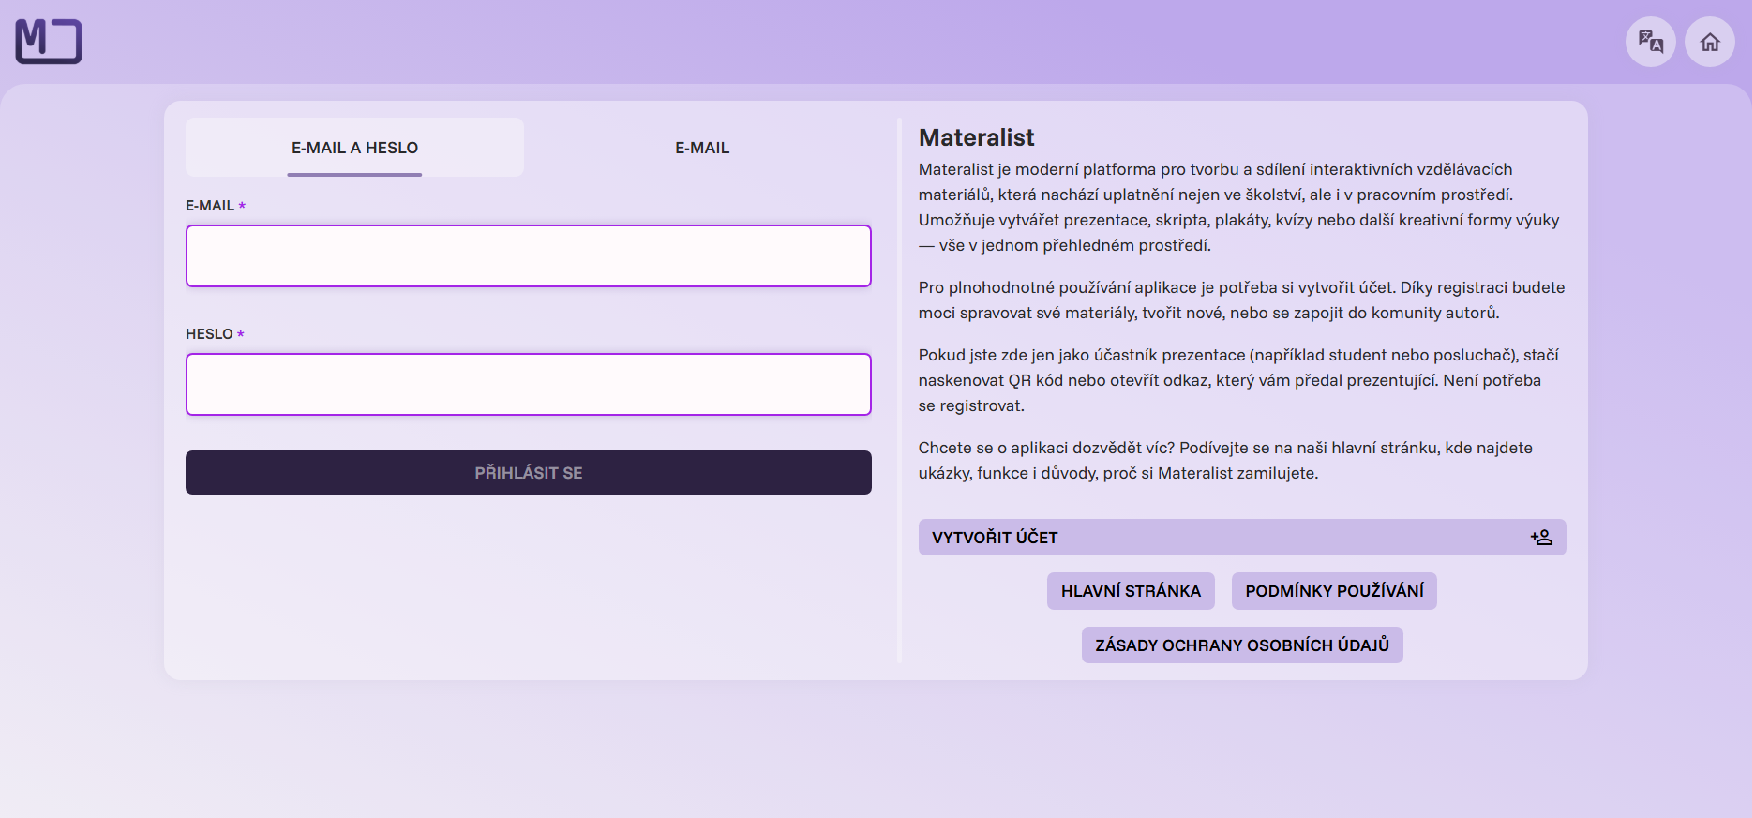
\includegraphics[width=1\textwidth,page=1]{media/appendix/uzivatelskeProstredi.pdf}
    \caption{Rozhraní aplikace pro přihlášení}
\end{figure}

\begin{figure}[ht!]
    \centering
    \includegraphics[width=1\textwidth,page=7]{media/appendix/uzivatelskeProstredi.pdf}
    \caption{Rozhraní aplikace pro vytvoření nového účtu}
\end{figure}


\begin{figure}[ht!]
    \centering
    \includegraphics[width=1\textwidth,page=2]{media/appendix/uzivatelskeProstredi.pdf}
    \caption{Rozhraní aplikace hlavního panelu s~materiály}
\end{figure}

\begin{figure}[ht!]
    \centering
    \includegraphics[width=1\textwidth,page=3]{media/appendix/uzivatelskeProstredi.pdf}
    \caption{Rozhraní aplikace s~editorem a snímky}
\end{figure}
\begin{figure}[ht!]
    \centering
    \includegraphics[width=1\textwidth,page=4]{media/appendix/uzivatelskeProstredi.pdf}
    \caption{Rozhraní aplikace s~předvolbami editoru}
\end{figure}

\begin{figure}[ht!]
    \centering
    \includegraphics[width=1\textwidth,page=5]{media/appendix/uzivatelskeProstredi.pdf}
    \caption{Rozhraní aplikace s~přehrávačem, zapnutým módem kreslením a kresbou}
\end{figure}


\begin{figure}
\centering
\begin{minipage}{.4\textwidth}
  \centering
    \includegraphics[width=1\textwidth,page=6]{media/appendix/uzivatelskeProstredi.pdf}
    \captionof{figure}{Rozhraní panelu s~materiály na telefonním zařízení}
\end{minipage}%
\hspace{0.1\textwidth}
\begin{minipage}{.4\textwidth}
  \centering
    \includegraphics[width=1\textwidth,page=10]{media/appendix/uzivatelskeProstredi.pdf}
    \captionof{figure}{Rozhraní aplikace s~editorem na telefonním zařízení}
\end{minipage}
\end{figure}


\begin{figure}[ht!]
    \centering
    \includegraphics[width=1\textwidth,page=8]{media/appendix/uzivatelskeProstredi.pdf}
    \caption{Rozhraní stránky s~technickou dokumentací, stránka pro vytváření rozšíření}
\end{figure}


\begin{figure}[ht!]
    \centering
    \includegraphics[width=1\textwidth,page=9]{media/appendix/uzivatelskeProstredi.pdf}
    \caption{Rozhraní hlavní stránky}
\end{figure}

\chapter{Testovací scénáře}\label{appendix:testovaciScenare}

% TC-U: uživatel (user)
% TC-E: tvořitel v~editoru
% TC-P: tvoritel v~prehravaci
% TC-W: sledovatel (watcher) 

% TC-U-1 registrace
% TC-U-2 prihlaseni heslo
% TC-U-3 prihlaseni email
% TC-U-4 změna jazyka
% TC-U-5 změna nastaveni
% TC-U-6 export dat

% TC-E-1 vytvoreni prázdného materialu
% TC-E-2 manipulace s~bloky + nastaveni vlastnosti
% TC-E-3 vlozeni vlastního obsahu
% TC-E-4 vlozeni obsahu z~banky
% TC-E-5 práce se snímky

% TC-E-6 práce s~editorem |||||| asi ne?

% TC-E-7 exportovani materialu JSON
% TC-E-8 exportovani materialu PDF
% TC-E-9 importovani materialu JSON
% TC-E-10 importovani materialu Markdown

% TC-E-11 nastaveni preferenci
% TC-E-12 nastaveni materialu

% TC-E-13 instalace a pouziti pluginu
% TC-E-14 odinstalovani pluginu

% TC-E-15 spusteni kolaborace, pouzivani
% TC-E-16 vytvoreni interaktivity 

% TC-E-17 oznaceni materilu jako vybraneho
% TC-E-18 oznaceni materialu jako nevybraneho

% TC-P-1 prochazeni materiálem
% TC-P-2 interakce s~prvky
% TC-P-3 kresleni
% TC-P-4 sdileni
% TC-P-5 zapnuti sledovani

% TC-W-1 pripojeni se ke sledovani
% TC-W-2 interakce s~interaktivními bloky

\vspace{1em}\noindent{\large\textbf{TC-U-1 -- Vytvoření uživatelského účtu}}

\textbf{Cíl}: Účelem je vytvoření uživatelského účtu uvnitř vytvořené aplikace.

\textbf{Časový limit}: do 5 minut

\textbf{Podmínky}: Aplikace je ve stavu, kdy uživatel není přihlášen a uživatel se nachází na hlavní stránce aplikace. Uživatel nemá zaregistrován žádný účet.

\textbf{Kroky}:

\begin{enumerate}[leftmargin=1.4cm]
    \item Účastník klikne na tlačítko \verb|Vytvořit si účet|.
    \item Účastník vyplní registrační formulář.
    \item Účastník formulář odešle kliknutím na tlačítko \verb|Registrovat se|.
    \item Účastník zkontroluje svoji e-mailovou schránku pro e-mail obsahující informace o~aktivaci.
    \item Účastník si pomocí pokynů z~e-mailu aktivuje účet.
\end{enumerate}

\textbf{Očekávané výsledky}:

\begin{enumerate}[leftmargin=1.4cm]
    \item Aplikace ho přesměruje automaticky na stránku s~přihlášením.
    \item V~aplikaci se vytvořil nový účet se zadanými údaji.
    \item Na zadaný e-mail aplikace odeslala e-mail se žádostí o~potvrzení e-mailu a aktivaci účtu.
    \item Účet je aktivovaný a lze se do něj přihlásit.
\end{enumerate}


\vspace{1em}\noindent{\large\textbf{TC-U-2 -- Přihlášení se pomocí e-mailu a hesla}}

\textbf{Cíl}: Účelem je přihlásit se do již existujícího účtu v~aplikaci pomocí e-mailu a hesla.

\textbf{Časový limit}: do 5 minut

\textbf{Podmínky}: Aplikace je ve stavu, kdy uživatel není přihlášen a uživatel se nachází na hlavní stránce. Účet již má účastník vytvořený a ví jeho přihlašovací údaje, například dle TC-U-1.

\textbf{Kroky}:

\begin{enumerate}[leftmargin=1.4cm]
    \item Účastník klikne na tlačítko \verb|E-mail a heslo|.
    \item Účastník vyplní svůj e-mail a heslo.
    \item Účastník formulář odešle kliknutím na tlačítko \verb|Přihlásit se|.
\end{enumerate}

\textbf{Očekávané výsledky}:

\begin{enumerate}[leftmargin=1.4cm]
    \item Aplikace ho přesměruje automaticky na stránku s~přihlášením.
    \item Uživatel je přihlášen.
    \item Je zobrazena hlavní stránka s~informacemi o~přihlášeném uživateli.
\end{enumerate}


\vspace{1em}\noindent{\large\textbf{TC-U-3 -- Přihlášení se pomocí e-mail s~potvrzením}}

\textbf{Cíl}: Účelem je přihlásit se do již existujícího účtu v~aplikaci pomocí e-mailu s~potvrzením.

\textbf{Časový limit}: do 5 minut

\textbf{Podmínky}: Aplikace je ve stavu, kdy uživatel není přihlášen a uživatel se nachází na hlavní stránce. Účet již má účastník vytvořený a ví jeho přihlašovací údaje, například dle TC-U-1.

\textbf{Kroky}:

\begin{enumerate}[leftmargin=1.4cm]
    \item Účastník zvolí možnost přihlášení pomocí e-mailu s~potvrzením.
    \item Účastník vyplní formulář s~e-mailem.
    \item Účastník formulář odešle pomocí kliknutí na tlačítko \verb|Přihlásit se|.
    \item Účastník si své své e-mailovou schránce vyzvedne informace o~přihlášení.
    \item Účastník do formuláře (či na nové stránce) vyplní kód, který mu přišel e-mailem.
    \item Účastník formulář odešle pomocí kliknutí na tlačítko \verb|Přihlásit se|.
\end{enumerate}

\textbf{Očekávané výsledky}:

\begin{enumerate}[leftmargin=1.4cm]
    \item Aplikace ho přesměruje automaticky na stránku s~přihlášením.
    \item Uživatel je přihlášen.
    \item Je zobrazena hlavní stránka s~informacemi o~přihlášeném uživateli.
\end{enumerate}


\vspace{1em}\noindent{\large\textbf{TC-U-4 -- Změna jazyka}}

\textbf{Cíl}: Účelem je, aby si uživatel v~aplikaci změnil jazyk na jiný.

\textbf{Časový limit}: do 2 minut

\textbf{Podmínky}: Aplikace je na nějaké stránce z~množiny: hlavní stránka, editor, přehrávač, přihlášení.

\textbf{Kroky}:

\begin{enumerate}[leftmargin=1.4cm]
    \item Účastník v~aplikaci nalezne tlačítko v~horní navigaci s~ikonou překladů.
    \item Účastník na tlačítko klikne a poté z~vyskakovacího menu vybere jiný jazyk, než je aktuálně nastaven.
\end{enumerate}

\textbf{Očekávané výsledky}:

\begin{enumerate}[leftmargin=1.4cm]
    \item V~aplikaci se změní jazyk na nově vybraný a všechny texty budou přeloženy v~daném jazyce.
\end{enumerate}






\vspace{1em}\noindent{\large\textbf{TC-U-5 -- Změna údajů účtu}}

\textbf{Cíl}: Uživatel si změn své jméno a heslo v~aplikaci.

\textbf{Časový limit}: do 5 minut

\textbf{Podmínky}: Uživatel je v~aplikaci přihlášen a zná svoje přihlašovací údaje. Uživatel je na panelu materiálů.

\textbf{Kroky}:

\begin{enumerate}[leftmargin=1.4cm]
    \item Uživatel nalezne tlačítko \verb|Nastavení| v~horní navigaci.
    \item Uživatel tlačítko zmáčkne a do formuláře zadá dle svého uvážení nové jméno a nové heslo v~aplikaci.
    \item Uživatel zadá své aktuálního heslo.
    \item Uživatel klikne na tlačítko \verb|Změnit údaje|.
    \item Poté uživatel přistoupí na hlavní stránku, kde nové údaje ověří.
\end{enumerate}

\textbf{Očekávané výsledky}:

\begin{enumerate}[leftmargin=1.4cm]
    \item Ve formuláři bylo automaticky vyplněno aktuální jméno v~aplikaci.
    \item Při správně zadaném aktuálním heslu se údaje změnily a jsou ihned vidět na hlavní stránce.
\end{enumerate}





\vspace{1em}\noindent{\large\textbf{TC-U-6 -- Exportování dat}}

\textbf{Cíl}: Uživatel si požádá o~exportování osobních údajů a dat z~aplikace a ty obdrží na e-mail.

\textbf{Časový limit}: do 5 minut

\textbf{Podmínky}: Uživatel je v~aplikaci přihlášen a nachází se na hlavní stránce. Uživatel v~nedávné době o~export osobních údajů nežádal.

\textbf{Kroky}:

\begin{enumerate}[leftmargin=1.4cm]
    \item Uživatel nalezne tlačítko \verb|Nastavení| v~horní navigaci.
    \item Uživatel tlačítko zmáčkne a ve formuláři pro export si přečte informace.
    \item Potom požádá o~export osobních údajů a dat stiskem na tlačítko \verb|Zažádat o export|.
    \item Uživatel počká na zpracování a čeká ve své e-mailové schránce.
    \item Uživatel přistoupí na stejnou stránku a pomocí tlačítka \verb|Stáhnout| obdrží archív s~osobními údaji.
    \item Uživatel si na počítači archív otevře a prozkoumá jejich obsah.
\end{enumerate}

\textbf{Očekávané výsledky}:

\begin{enumerate}[leftmargin=1.4cm]
    \item Aplikace požadavek zpracuje a odešle e-mail.
    \item Stáhnutý archív bude obsahovat minimálně dva soubory  \verb|user.json| a \verb|preferences.json| s~údaji uživatele z~aplikace.
\end{enumerate}

\textbf{Poznámky}:

\begin{itemize}[leftmargin=1.4cm]
    \item Aplikace nemusí stihnout v~reálném čase požadavek zpracovat, testovací verze aplikace musí mít vypnutý zpomalovač požadavků a případně tomuto exportu dát větší prioritu.
\end{itemize}






\vspace{1em}\noindent{\large\textbf{TC-E-1 -- Vytvoření prázdného materiálu}}

\textbf{Cíl}: Uživatel v~aplikaci vytvoří nový materiál bez obsahu.

\textbf{Časový limit}: do 2 minut

\textbf{Podmínky}: Uživatel je v~aplikaci přihlášen a nachází se na hlavní stránce.

\textbf{Kroky}:

\begin{enumerate}[leftmargin=1.4cm]
    \item Uživatel nalezne tlačítko přidání materiálu pod ikonou znaku plus.
    \item Uživatel na tlačítko klikne a uvnitř vyskakovacího okna vybere možnost nového materiálu.
    \item Uživatel v~editoru klikne na tlačítko panelu a na hlavní stránce znovu otevře stejný materiál.
\end{enumerate}

\textbf{Očekávané výsledky}:

\begin{enumerate}[leftmargin=1.4cm]
    \item Aplikace vytvoří prázdný materiál a uživatele na něj přesměruje.
    \item Materiál bude k~dispozici na hlavní stránce.
\end{enumerate}






\vspace{1em}\noindent{\large\textbf{TC-E-2 -- Tvorba bloků a jejich manipulace}}

\textbf{Cíl}: Uživatel v~materiálu přidá základní bloky -- text a tvar. Bloky umístí do editoru. Textu změní obsah, barvu a podtržení. Bloku tvaru změní tvar a barvu. Tvar otočí o~90 stupňů a zvětší ho. 

\textbf{Časový limit}: do 10 minut

\textbf{Podmínky}:  Uživatel je v~aplikaci přihlášen a nachází se na hlavní stránce. Uživatel má vytvořený prázdný materiál, jako například v~TC-E-1.

\vspace{1em}
\textbf{Kroky}:

\begin{enumerate}[leftmargin=1.4cm]
    \item Účastník na hlavní stránce otevře materiál klikem na jeho kartičku.
    \item Účastník v~editoru nalezne panel pro přidávání bloků s~ikonou plus ve čtverci.
    \item Účastník do editoru přidá blok tvaru a textu.
    \item Účastník upraví text dvojklikem na něm.
    \item Účastník označí v~textu slova a jim změní pomocí postranního panelu s~vlastnostmi barvu a podtržení.
    \item Účastník označí blok, v~panelu vlastností změní tvar a barvu.
    \item Účastník pomocí panelu vlastností či pomocí nástrojů uvnitř editoru změní rotaci a velikost.
\end{enumerate}

\textbf{Očekávané výsledky}:

\begin{enumerate}[leftmargin=1.4cm]
    \item Na prvním snímku v~materiálu je blok textu a tvaru.
    \item Text má vlastní obsah, který je obarven a podtržen.
    \item Tvar je pootočen, zvětšen, je obarven a má nastaven nějaký tvar. 
\end{enumerate}






\vspace{1em}\noindent{\large\textbf{TC-E-3 -- Přidání vlastního obsahu}}

\textbf{Cíl}: Uživatel v~materiálu nahraje vlastní obrázek a ten vloží do materiálu.

\textbf{Časový limit}: do 5 minut

\textbf{Podmínky}:  Uživatel je v~aplikaci přihlášen a nachází se na hlavní stránce. Uživatel má vytvořený prázdný materiál, jako například v~TC-E-1. Uživatel má na počítači obrázek, který nahraje do aplikace.

\textbf{Kroky}:

\begin{enumerate}[leftmargin=1.4cm]
    \item Účastník na hlavní stránce otevře materiál klikem na jeho kartičku.
    \item Účastník v~editoru nalezne panel pro přidávání obsahu s~ikonou multimédií.
    \item V~postranním panelu uživatel klikne na tlačítko \verb|Nahrát obsah|.
    \item Účastník v~počítači vybere soubor a nahraje ho.
    \item Účastník v~postranním menu obrázek vybere a přidá ho do materiálu.
\end{enumerate}

\textbf{Očekávané výsledky}:

\begin{enumerate}[leftmargin=1.4cm]
    \item Na prvním snímku v~materiálu je nový blok s~obrázkem od uživatele.
    \item Obrázek se nahrál do aplikace.
\end{enumerate}






\vspace{1em}\noindent{\large\textbf{TC-E-4 -- Přidání obsahu z~banky}}

\textbf{Cíl}: Uživatel v~materiálu nahraje obrázek z~banky obsahu.

\textbf{Časový limit}: do 5 minut

\textbf{Podmínky}:  Uživatel je v~aplikaci přihlášen a nachází se na hlavní stránce. Uživatel má vytvořený prázdný materiál, jako například v~TC-E-1.

\textbf{Kroky}:

\begin{enumerate}[leftmargin=1.4cm]
    \item Účastník na hlavní stránce otevře materiál klikem na jeho kartičku.
    \item Účastník v~editoru nalezne panel pro přidávání obsahu s~ikonou glóbusu.
    \item V~postranním panelu uživatel vybere, zda chce nahrávat obrázek či animovaný GIF.
    \item Účastník v~postranním panelu vybere obsah z~banky (obrázek či animovaný GIF) a přidá ho do materiálu.
\end{enumerate}

\textbf{Očekávané výsledky}:

\begin{enumerate}[leftmargin=1.4cm]
    \item Na prvním snímku v~materiálu je nový blok s~vybraným obrázkem od uživatele z~banky animovaných GIF či obrázků.
\end{enumerate}






\vspace{1em}\noindent{\large\textbf{TC-E-5 -- Práce se snímky}}

\textbf{Cíl}: Uživatel v~materiálu přidá dva další snímky, změní jim pozadí a velikost, a do každého snímku vloží nějaký obsah.

\textbf{Časový limit}: do 5 minut

\textbf{Podmínky}:  Uživatel je v~aplikaci přihlášen a nachází se na hlavní stránce. Uživatel má vytvořený prázdný materiál, jako například v~TC-E-1.

\textbf{Kroky}:

\begin{enumerate}[leftmargin=1.4cm]
    \item Účastník na hlavní stránce otevře materiál klikem na jeho kartičku.
    \item Účastník v~editoru nalezne panel snímků s~ikonou kartiček.
    \item V~postranním panelu účastník klikne na tlačítko \verb|Přidat snímek| dvakrát.
    \item V~postranním panelu účastník otevře nastavení snímku a změní jim barvu pozadí a jejich velikost.
    \item Účastník prochází mezi snímky a do každého z~nich vloží obsah.
\end{enumerate}

\textbf{Očekávané výsledky}:

\begin{enumerate}[leftmargin=1.4cm]
    \item Materiál má vytvořené tři snímky, kde v~každém z~nich je jiný obsah, mají jiné pozadí a jinou velikost.
\end{enumerate}






\vspace{1em}\noindent{\large\textbf{TC-E-6 -- Exportování materiálu do JSON}}

\textbf{Cíl}: Uživatel exportuje materiál do formátu JSON pomocí aplikace.

\textbf{Časový limit}: do 2 minut

\textbf{Podmínky}:  Uživatel je v~aplikaci přihlášen a nachází se na hlavní stránce. Uživatel má vytvořený materiál s~nějakým obsahem, stejně jako například po TC-E-5.

\textbf{Kroky}:

\begin{enumerate}[leftmargin=1.4cm]
    \item Účastník na hlavní stránce otevře materiál klikem na jeho kartičku.
    \item Účastník v~horním navigaci najde tlačítko \verb|Sdílení| a klikne na něj.
    \item Účastník vybere možnost \verb|Export materiálu| a poté vybere možnost JSON.
    \item Účastník ověří, že soubor není prázdný tím, že ho otevře.
\end{enumerate}

\textbf{Očekávané výsledky}:

\begin{enumerate}[leftmargin=1.4cm]
    \item Materiál se automaticky stáhne pod názvem materiálu s~příponou \verb|.json|.
\end{enumerate}




\vspace{1em}\noindent{\large\textbf{TC-E-7 -- Exportování materiálu do PDF}}

\textbf{Cíl}: Uživatel exportuje materiál do formátu PDF pomocí aplikace.

\textbf{Časový limit}: do 10 minut

\textbf{Podmínky}:  Uživatel je v~aplikaci přihlášen a nachází se na hlavní stránce. Uživatel má vytvořený materiál s~nějakým obsahem, stejně jako například po TC-E-5.

\textbf{Kroky}:

\begin{enumerate}[leftmargin=1.4cm]
    \item Účastník na hlavní stránce otevře materiál klikem na jeho kartičku.
    \item Účastník v~horním navigaci najde tlačítko \verb|Sdílení| a klikne na něj.
    \item Účastník vybere možnost \verb|Export materiálu| a poté vybere možnost \verb|PDF|.
    \item Účastník ověří, že soubor není prázdný tím, že ho otevře.
\end{enumerate}

\textbf{Očekávané výsledky}:

\begin{enumerate}[leftmargin=1.4cm]
    \item Materiál se automaticky stáhne pod názvem materiálu s~příponou \verb|.pdf|.
    \item Vytvořený soubor obsahuje přesnou kopii vytvořených prvků s~danou vizualizací a velikostmi.
\end{enumerate}

\textbf{Poznámky}:

\begin{itemize}[leftmargin=1.4cm]
    \item Aplikace nemusí stihnout v~reálném čase požadavek zpracovat, protože exportování závisí na využití vykreslovače na serveru.
\end{itemize}





\vspace{1em}\noindent{\large\textbf{TC-E-8 -- Importování materiálu z~JSON}}

\textbf{Cíl}: Uživatel do aplikace importuje materiál z~formátu JSON.

\textbf{Časový limit}: do 5 minut

\textbf{Podmínky}:  Uživatel je v~aplikaci přihlášen a nachází se na hlavní stránce. Uživatel má staženou zálohu jiného materiálu, například dle scénáře TC-E-6.

\textbf{Kroky}:

\begin{enumerate}[leftmargin=1.4cm]
    \item Uživatel nalezne tlačítko přidání materiálu pod ikonou znaku plus.
    \item Uživatel na tlačítko klikne a uvnitř vyskakovacího okna vybere možnost importu materiálu.
    \item Účastník v~počítači vybere soubor a nahraje ho.
    \item Účastník projde vytvořený materiál zda souhlasí s~exportovanou verzí.
\end{enumerate}

\vspace{2em}
\textbf{Očekávané výsledky}:

\begin{enumerate}[leftmargin=1.4cm]
    \item Materiál se vytvořil dle přiloženého souboru typu JSON.
\end{enumerate}






\vspace{1em}\noindent{\large\textbf{TC-E-9 -- Importování materiálu z~Markdown}}

\textbf{Cíl}: Uživatel do aplikace importuje materiál z~formátu Markdown.

\textbf{Časový limit}: do 10 minut

\textbf{Podmínky}:  Uživatel je v~aplikaci přihlášen a nachází se na hlavní stránce. Uživatel ví, jak vypadá formát JSON a je schopný ho samostatně napsat.

\textbf{Kroky}:

\begin{enumerate}[leftmargin=1.4cm]
    \item Uživatel nalezne tlačítko přidání materiálu pod ikonou znaku plus.
    \item Uživatel na tlačítko klikne a uvnitř vyskakovacího okna vybere možnost importu materiálu.
    \item Uživatel si na počítači založí soubor s~příponou \verb|md|.
    \item Uživatel dle pokynů vytvoří nějakou strukturu prezentace za pomocí nadpisu H1, H2 a textových tagů jak je list, tučné písmo, podtržení a další.
    \item Účastník v~počítači vybere soubor a nahraje ho.
    \item Účastník projde vytvořený materiál zda souhlasí s~tím, co uvedl v~souboru.
\end{enumerate}

\textbf{Očekávané výsledky}:

\begin{enumerate}[leftmargin=1.4cm]
    \item Materiál se vytvořil dle přiloženého souboru typu Markdown a obsahuje vše, co uživatel zadal.
\end{enumerate}





\vspace{1em}\noindent{\large\textbf{TC-E-10 -- Nastavení preferencí}}

\textbf{Cíl}: Uživatel si změní preference v~editoru a vyzkouší změněné možnosti.

\textbf{Časový limit}: do 5 minut

\textbf{Podmínky}:  Uživatel je v~aplikaci přihlášen a nachází se na hlavní stránce.  Uživatel má vytvořený materiál s~nějakým obsahem, stejně jako například po TC-E-5.

\textbf{Kroky}:

\begin{enumerate}[leftmargin=1.4cm]
    \item Účastník na hlavní stránce otevře materiál klikem na jeho kartičku.
    \item Účastník v~horním navigaci najde tlačítko \verb|Předvolby| a klikne na něj.
    \item Účastník si přečte možnosti nastavení a dle svého uvážení ho upraví. 
    \item Účastník klikem na tlačítko \verb|Uložit| uloží své nastavení.
    \item Změněné nastavení účastník vyzkouší přímo v~editoru.
\end{enumerate}

\textbf{Očekávané výsledky}:

\begin{enumerate}[leftmargin=1.4cm]
    \item Uživatelské předvolby a preference editoru se změnily a propsali se do aktuálně otevřeného editoru. 
\end{enumerate}




\vspace{1em}\noindent{\large\textbf{TC-E-11 -- Nastavení materiálu}}

\textbf{Cíl}: Uživatel si pro materiál změní nastavení. Změní jméno, viditelnost, průchod a zobrazení materiálu.

\textbf{Časový limit}: do 5 minut

\textbf{Podmínky}:  Uživatel je v~aplikaci přihlášen a nachází se na hlavní stránce.  Uživatel má vytvořený materiál s~nějakým obsahem, stejně jako například po TC-E-5.

\textbf{Kroky}:

\begin{enumerate}[leftmargin=1.4cm]
    \item Účastník na hlavní stránce otevře materiál klikem na jeho kartičku.
    \item Účastník v~horním navigaci najde tlačítko \verb|Sdílení| a klikne na něj.
    \item Poté zvolí možnost \verb|Nastavení materiálu|.
    \item Účastník si přečte možnosti nastavení a dle svého uvážení je upraví. 
    \item Účastník klikem na tlačítko \verb|Uložit| uloží své nastavení.
    \item Změněné nastavení účastník vyzkouší přímo v~přehrávači.
\end{enumerate}

\textbf{Očekávané výsledky}:

\begin{enumerate}[leftmargin=1.4cm]
    \item Nastavení materiálu se změnilo na vyplněné hodnoty.
    \item Pokud uživatel nastavil materiál jako veřejný, je možné ho navštívit se odkazem pro sdílení.
\end{enumerate}




\vspace{1em}\noindent{\large\textbf{TC-E-12 -- Instalace a použití rozšíření}}

\textbf{Cíl}: Uživatel si v~materiálu nainstaluje rozšíření \verb|Word wall| a použije ho. Tedy přidá blok do materiálu.

\textbf{Časový limit}: do 5 minut

\textbf{Podmínky}:  Uživatel je v~aplikaci přihlášen a nachází se na hlavní stránce.  Uživatel má vytvořený prázdný materiál. V~aplikaci se nachází ukázkové rozšíření \verb|Word wall|.

\textbf{Kroky}:

\begin{enumerate}[leftmargin=1.4cm]
    \item Účastník na hlavní stránce otevře materiál klikem na jeho kartičku.
    \item Účastník v~boční navigaci najde tlačítko \verb|Spravovat pluginy| a klikne na něj.
    \item Poté zvolí možnost \verb|Procházet pluginy|.
    \item Účastník vybere a nainstaluje rozšíření \verb|Word wall|.
    \item Účastník v~navigaci pod rozšířením otevře panel rozšíření a zvolí možnost přidání bloku do materiálu.
    \item Účastník vyzkouší rozšíření přímo v~přehrávači.
\end{enumerate}

\textbf{Očekávané výsledky}:

\begin{enumerate}[leftmargin=1.4cm]
    \item Materiál nyní obsahuje nainstalované rozšíření nejnovější možné verze.
    \item Materiál obsahuje vlastní blok pluginu a rozšíření s~blokem funguje.
\end{enumerate}



\vspace{1em}\noindent{\large\textbf{TC-E-13 -- Odinstalování rozšíření}}

\textbf{Cíl}: Uživatel si v~materiálu odinstaluje rozšíření \verb|Word wall|.

\textbf{Časový limit}: do 5 minut

\textbf{Podmínky}:  Aplikace je v~stavu po provedení scénáře TC-E-13. Uživatel se nachází na stránce materiálu.

\textbf{Kroky}:

\begin{enumerate}[leftmargin=1.4cm]
    \item Účastník v~boční navigaci najde tlačítko \verb|Spravovat pluginy| a klikne na něj.
    \item Účastník odinstaluje rozšíření \verb|Word wall|.
    \item Účastník odebere blok rozšíření z~materiálu.
\end{enumerate}

\textbf{Očekávané výsledky}:

\begin{enumerate}[leftmargin=1.4cm]
    \item Materiál neobsahuje žádné nainstalované rozšíření.
\end{enumerate}




\vspace{1em}\noindent{\large\textbf{TC-E-14 -- Kolaborace}}

\textbf{Cíl}: Uživatel si v~materiálu zapne kolaboraci a zkusí editovat materiál z~dvou různých oken prohlížeče. 

\textbf{Časový limit}: do 5 minut

\textbf{Podmínky}:  Uživatel je v~aplikaci přihlášen a nachází se na hlavní stránce.  Uživatel má vytvořený materiál s~nějakým obsahem, stejně jako například po TC-E-5.

\textbf{Kroky}:

\begin{enumerate}[leftmargin=1.4cm]
    \item Účastník na hlavní stránce otevře materiál klikem na jeho kartičku.
    \item Účastník otevře stejnou stránku v~jiném okně prohlížeče.
    \item Účastník provede změny na nějakém snímku v~různých instancích aplikace.
    \item Účastník může zkontrolovat připojené uživatele pomocí tlačítka uživatelů v~horní části navigace.
\end{enumerate}

\textbf{Očekávané výsledky}:

\begin{enumerate}[leftmargin=1.4cm]
    \item Materiál se otevře v~obou oknech prohlížeče.
    \item Materiál lze upravovat z~obou instancí a změny se v~reálném čase propisují do druhého okna.
    \item Blok v~snímku nejde upravovat oběma instancemi najednou.
\end{enumerate}





\vspace{1em}\noindent{\large\textbf{TC-E-15 -- Vytvoření interaktivity}}

\textbf{Cíl}: Uživatel si ve snímku v~materiálu vytvoři na bloku tvaru interaktivitu: při kliku na daný tvar se otevře stránka materalist.com v~novém okně.

\textbf{Časový limit}: do 5 minut

\textbf{Podmínky}:  Uživatel je v~aplikaci přihlášen a nachází se na hlavní stránce.  Uživatel má vytvořený materiál s~nějakým obsahem, stejně jako například po TC-E-5.

\textbf{Kroky}:

\begin{enumerate}[leftmargin=1.4cm]
    \item Účastník na hlavní stránce otevře materiál klikem na jeho kartičku.
    \item Účastník přidá blok tvaru.
    \item Účastník v~panelu vlastností přidá interaktivitu a nastaví hodnoty:
    \begin{itemize}
        \item \textbf{Událost}: Kliknuto.
        \item \textbf{Akce}: Otevřít odkaz.
        \item \textbf{Odkaz}: https://materalist.com
        \item \textbf{Pouze}: Vždy.
    \end{itemize}
    \item Účastník vyzkouší interaktivitu v~přehrávači.
\end{enumerate}

\textbf{Očekávané výsledky}:

\begin{enumerate}[leftmargin=1.4cm]
    \item Materiál obsahuje blok s~danou interaktivitou.
    \item Po kliku na blok v~přehrávači se otevře nová stránka s~adresou materalist.com.
\end{enumerate}




\vspace{1em}\noindent{\large\textbf{TC-E-16 -- Označení materiálu jako ukázkového}}

\textbf{Cíl}: Uživatel si v~aplikaci označí nějaký svůj materiál jako ukázkový, aby se zobrazil na ukázkových materiálech.

\textbf{Časový limit}: do 5 minut

\textbf{Podmínky}:  Uživatel je v~aplikaci přihlášen a nachází se na hlavní stránce.  Uživatel má vytvořený materiál s~nějakým obsahem, stejně jako například po TC-E-5.

\textbf{Kroky}:

\begin{enumerate}[leftmargin=1.4cm]
    \item Účastník na hlavní stránce otevře ukázkové materiály.
    \item Účastník najde tlačítko pro přidání, označeno ikonou tvaru plus.
    \item Účastník vybere materiál, který chce označit jako ukázkový a odešle formulář tlačítkem \verb|Přidat|.
    \item Účastník uvidí vybraný materiál v~seznamu.
\end{enumerate}

\textbf{Očekávané výsledky}:

\begin{enumerate}[leftmargin=1.4cm]
    \item Materiál obsahuje blok s~danou interaktivitou.
    \item Po kliku na blok v~přehrávači se otevře nová stránka s~adresou materalist.com.
\end{enumerate}

\textbf{Poznámky}:

\begin{itemize}[leftmargin=1.4cm]
    \item Aplikace v~daný moment může nezpracovat žádost o~umístění do ukázkových materiálů. Pro testování je vhodné vypnout prodlevu k~umístění.
\end{itemize}





\vspace{1em}\noindent{\large\textbf{TC-E-17 -- Přidání spoluúčastníka editace}}

\textbf{Cíl}: Uživatel si v~aplikaci přidá do svého materiálu spoluúčastníka editace.

\textbf{Časový limit}: do 5 minut

\textbf{Podmínky}:  Uživatel je v~aplikaci přihlášen a nachází se na hlavní stránce.  Uživatel má vytvořený materiál s~nějakým obsahem, stejně jako například po TC-E-5. V~aplikaci existuje další účet, který lze do materiálu přidat (a ten pozorovatel testování předloží účastníkovi).

\textbf{Kroky}:

\begin{enumerate}[leftmargin=1.4cm]
    \item Účastník na hlavní stránce otevře materiál klikem na jeho kartičku.
    \item Účastník v~horní navigaci vybere možnosti nastavení.
    \item Ve vyskakovacím okně vybere možnost editace spolu účastníku editace.
    \item Účastník zadá e-mail, který mu poskytne pozorovatel testování.
    \item Pozorovatel se připojí a zkusí práci s~editorem.
\end{enumerate}

\textbf{Očekávané výsledky}:

\begin{enumerate}[leftmargin=1.4cm]
    \item Do materiálu se dostane testovací účet a může editovat jednotlivé snímky.
\end{enumerate}






\vspace{1em}\noindent{\large\textbf{TC-P-1 -- Procházení materiálu}}

\textbf{Cíl}: Uživatel si v~aplikaci otevře materiál a bude ho procházet.

\textbf{Časový limit}: do 5 minut

\textbf{Podmínky}:  Uživatel je v~aplikaci přihlášen a nachází se na hlavní stránce.  Uživatel má vytvořený materiál s~nějakým obsahem, stejně jako například po TC-E-5.

\textbf{Kroky}:

\begin{enumerate}[leftmargin=1.4cm]
    \item Účastník na hlavní stránce otevře materiál klikem na jeho kartičku.
    \item V~horní navigaci účastník najde tlačítko \verb|Náhled| a klikem na něj.
    \item Na stránce v~přehrávači uživatel prochází materiálem tlačítky v~navigaci, pomocí šipek na klávesnici nebo kliky na snímek.
\end{enumerate}

\textbf{Očekávané výsledky}:

\begin{enumerate}[leftmargin=1.4cm]
    \item Materiál se otevřel v~přehrávači a lze ním procházet.
\end{enumerate}



\vspace{1em}\noindent{\large\textbf{TC-P-2 -- Interakce s~prvky}}

\textbf{Cíl}: Uživatel si v~aplikaci otevře materiál a bude manipulovat s~prvkem s~interaktivitou.

\textbf{Časový limit}: do 5 minut

\textbf{Podmínky}:  Uživatel je v~aplikaci přihlášen a nachází se na hlavní stránce.  Uživatel má vytvořený materiál s~nějakým obsahem a blokem s~interaktivitou, stejně jako například po scénáři TC-E-15.

\textbf{Kroky}:

\begin{enumerate}[leftmargin=1.4cm]
    \item Účastník na hlavní stránce otevře materiál klikem na jeho kartičku.
    \item V~horní navigaci účastník najde tlačítko \verb|Náhled| a klikem na něj.
    \item Na stránce v~přehrávači uživatel prochází materiálem tlačítky v~navigaci, pomocí šipek na klávesnici nebo kliky na snímek.
    \item Účastník najde blok s~tvarem a interaktivitou a klikne na něj.
\end{enumerate}

\textbf{Očekávané výsledky}:

\begin{enumerate}[leftmargin=1.4cm]
    \item Materiál lze procházet a s~blokem lze interagovat.
    \item Po kliknutí na materiál se otevře nová stránka materalist.com.
\end{enumerate}






\vspace{1em}\noindent{\large\textbf{TC-P-3 -- Kreslení}}

\textbf{Cíl}: Uživatel si v~aplikaci otevře materiál a v~přehrávači bude kreslit na snímek pomocí různých barev a velikostí.

\textbf{Časový limit}: do 5 minut

\textbf{Podmínky}:  Uživatel je v~aplikaci přihlášen a nachází se na hlavní stránce.  Uživatel má vytvořený materiál s~nějakým obsahem, stejně jako například po TC-E-5.

\textbf{Kroky}:

\begin{enumerate}[leftmargin=1.4cm]
    \item Účastník na hlavní stránce otevře materiál klikem na jeho kartičku.
    \item V~horní navigaci účastník najde tlačítko \verb|Náhled| a klikem na něj.
    \item Na stránce v~přehrávači uživatel nalezne tlačítko \verb|Kreslení| a klikne na něj.
    \item Pomocí možností v~dolní navigaci na snímku uživatel mění velikost, barvy, stabilizaci a další.
    \item Účastník na snímku něco nakreslí a označí.
\end{enumerate}

\textbf{Očekávané výsledky}:

\begin{enumerate}[leftmargin=1.4cm]
    \item Materiál lze procházet a na plátno lze kreslit.
    \item Možnosti kreslení (barva, velikost, stabilizace, guma) fungují.
\end{enumerate}






\vspace{1em}\noindent{\large\textbf{TC-P-4 -- Sdílení materiálu}}

\textbf{Cíl}: Uživatel si v~aplikaci otevře materiál a v~přehrávači zkopíruje odkaz pro sdílení. Odkaz účastník vyzkouší v~anonymním okně.

\textbf{Časový limit}: do 5 minut

\textbf{Podmínky}:  Uživatel je v~aplikaci přihlášen a nachází se na hlavní stránce.  Uživatel má vytvořený materiál s~nějakým obsahem, stejně jako například po TC-E-5. Materiál musí být nastaven jako veřejný.

\textbf{Kroky}:

\begin{enumerate}[leftmargin=1.4cm]
    \item Účastník na hlavní stránce otevře materiál klikem na jeho kartičku.
    \item V~horní navigaci účastník najde tlačítko \verb|Náhled| a klikem na něj.
    \item Na stránce v~přehrávači uživatel nalezne tlačítko \verb|Sdílení| a klikne na něj.
    \item Účastník zkopíruje odkaz.
    \item Účastník otevře anonymní okno a otevře v~něm materiál z~odkazu.
\end{enumerate}

\textbf{Očekávané výsledky}:

\begin{enumerate}[leftmargin=1.4cm]
    \item Materiál lze procházet.
    \item Účastníkovi se zkopíroval odkaz pro sdílení.
    \item Účastník v~anonymním režimu v~prohlížeči funguje zobrazení materiálu.
\end{enumerate}





\vspace{1em}\noindent{\large\textbf{TC-P-5 -- Zapnutí sledování}}

\textbf{Cíl}: Uživatel si v~aplikaci otevře materiál a v~přehrávači zkopíruje odkaz pro sdílení se sledováním. Odkaz účastník vyzkouší v~anonymním okně.

\textbf{Časový limit}: do 5 minut

\textbf{Podmínky}:  Uživatel je v~aplikaci přihlášen a nachází se na hlavní stránce.  Uživatel má vytvořený materiál s~nějakým obsahem, stejně jako například po TC-E-5. Materiál musí být nastaven jako veřejný.

\textbf{Kroky}:

\begin{enumerate}[leftmargin=1.4cm]
    \item Účastník na hlavní stránce otevře materiál klikem na jeho kartičku.
    \item V~horní navigaci účastník najde tlačítko \verb|Náhled| a klikem na něj.
    \item Na stránce v~přehrávači uživatel nalezne tlačítko \verb|Sdílení| a klikne na něj.
    \item Účastník vybere možnost \verb|Sdílení odkazu pro sledování|.
    \item Účastník zkopíruje odkaz.
    \item Účastník otevře anonymní okno a otevře v~něm materiál z~odkazu.
    \item V~původním okně se účastník zkusí pohybovat mezi snímky a zkusí něco nakreslit. 
\end{enumerate}

\textbf{Očekávané výsledky}:

\begin{enumerate}[leftmargin=1.4cm]
    \item Materiál lze procházet.
    \item Účastníkovi se zkopíroval odkaz pro sdílení se sledováním.
    \item Účastník v~anonymním režimu v~prohlížeči funguje zobrazení materiálu.
    \item Procházení snímku a kresba se synchronizuje od prezentujícího.
\end{enumerate}




\vspace{1em}\noindent{\large\textbf{TC-P-6 -- Připojení se k~sledování}}

\textbf{Cíl}: Uživatel se pomocí odkazu od pozorovatele testování připojí ke sledování a zkouší funkcionality módu sledujícího.

\textbf{Časový limit}: do 5 minut

\textbf{Podmínky}:  V~aplikaci existuje testovací účet, ke kterému má přístup pozorovatel a pro tento účet existuje ukázkový materiál. 

\textbf{Kroky}:

\begin{enumerate}[leftmargin=1.4cm]
    \item Pozorovatel zapne prezentování materiálu.
    \item Pozorovatel zkopíruje či ukáže kód na připojení účastníkovi.
    \item Účastník odkaz otevře a případně zadá kód.
    \item Pozorovatel v~materiálu používá různé funkcionality, jako např. kreslení, průchod snímky a podobně.
    \item Účastník zkusí změnu jazyka, interakci s~prvky a další funkcionality.
\end{enumerate}

\textbf{Očekávané výsledky}:

\begin{enumerate}[leftmargin=1.4cm]
    \item Materiál je v~módu prezentace pro pozorovatele.
    \item Účastník se připojí ke sledování materiálu.
    \item Průchod snímky a kreslení se synchronizuje mezi zařízeními.
    \item S~interaktivními prvky materiálu můžou interagovat obě zařízení.
\end{enumerate}

\chapter{Zadání diplomové práce z~IS KOS}

V souladu s~novým metodickým pokynem ČVUT připojuji zadání práce, které bylo vytvořeno prostřednictvím informačního systému KOS. 
Toto zadání bylo možné vytvořit až v~průběhu zpracovávání práce, a z~tohoto důvodu je ponecháno původní zadání, které schválil Ing. Jaroslav Kuchař, Ph.D., na začátku této práce.

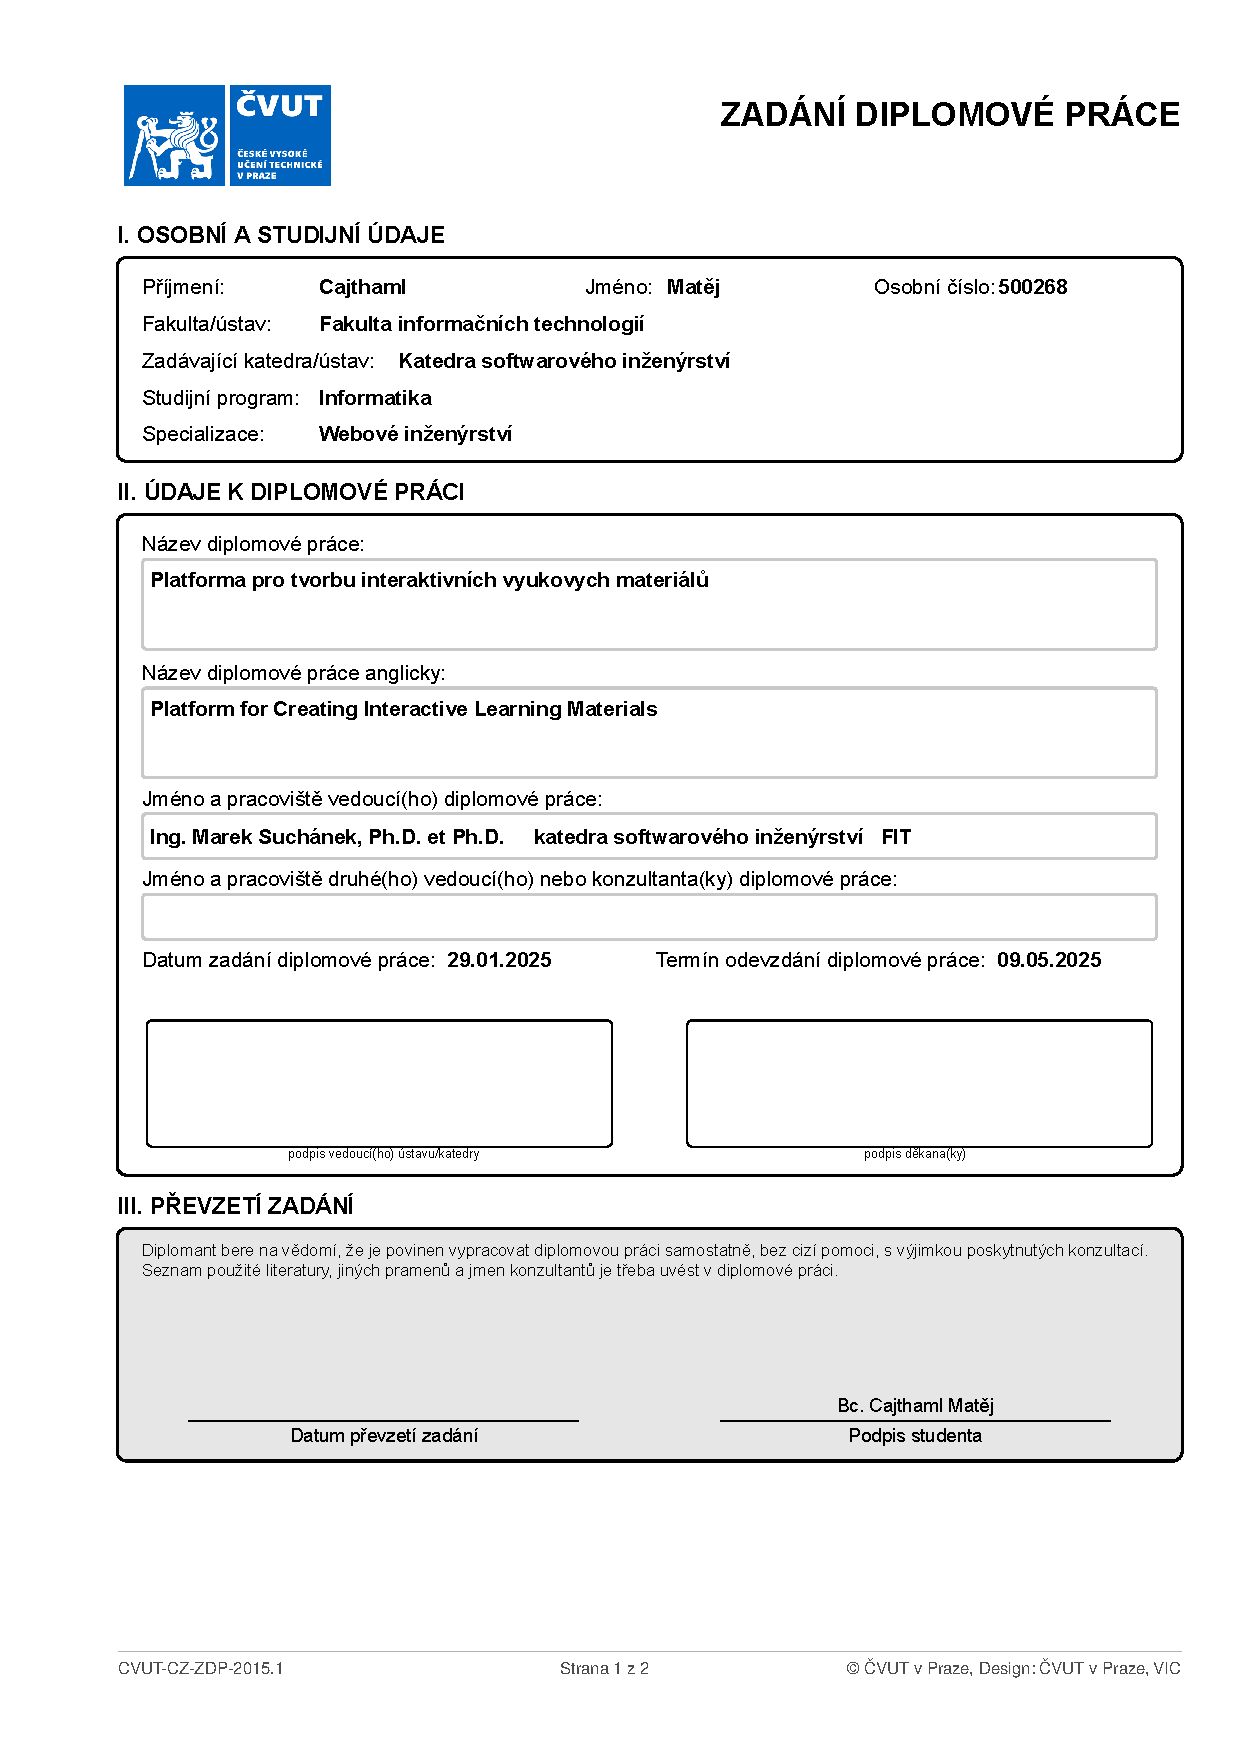
\includepdf[pages={1-}]{zadani.pdf} % include `appendix.tex' from `text/' subdirectory

\backmatter % do not remove this command

{
    \setlength{\emergencystretch}{3em} 
    \def\UrlBreaks{\do\/\do\-\do\_}
    \printbibliography
}

\chapter{Obsah přiloženého archivu}


\dirtree{%
    .1 readme.txt\DTcomment{stručný popis obsahu archivu}.
    .1 install.txt\DTcomment{instalační příručka a zprovoznění aplikace}.
    .1 links.txt\DTcomment{odkazy k veřejně dostupné verzi práce}.
    .1 frames.fig\DTcomment{zdrojová forma návrhových obrazovek}.
    .1 text\DTcomment{zdrojová forma práce ve formátu \LaTeX{}}.
    .1 examples\DTcomment{lokální zálohy ukázkových materiálů v JSON}.
    .1 testing\DTcomment{CSV data z uživatelského testování}.
    .1 platform\DTcomment{zdrojové kódy jednotlivých částí aplikace}.
        .2 docker-compose.yml\DTcomment{soubor nastavení pro produkční nasazení}.
        .2 docker-compose.dev.yml\DTcomment{soubor nastavení pro lokální nasazení}.
        .2 .gitlab-ci.yml\DTcomment{soubor nastavení pro CI/CD pro GitLab}.
        .2 .env\DTcomment{proměnné pro lokální nasazení}.
        .2 server\DTcomment{zdrojové kódy serverovou}.
        .2 client\DTcomment{zdrojové kódy pro klientskou část}.
        .2 homepage\DTcomment{zdrojové kódy pro hlavní stránku}.
        .2 docs\DTcomment{zdrojové kódy pro dokumentaci a její stránku}.
        .2 scripts\DTcomment{kódové skripty použity během vývoje}.
        .2 plugins\DTcomment{zdrojové kódy jednotlivých rozšíření pro platformu}.
} % include `medium.tex' from `text/' subdirectory

\end{document}
